\documentclass{beamer}

\usepackage{amsmath,amssymb}
\usepackage{color}
\usepackage[UTF8,noindent]{ctexcap}
\usepackage{textcomp}
%\usepackage[timeinterval=1]{tdclock}%显示当前时间宏包
%%\usetheme{AnnArbor}
%\usetheme{Antibes}
%\usetheme{CambridgeUS}
%\usetheme{Copenhagen}
%\usetheme{Darmstadt}%!
%\usetheme{Dresden}
%\usetheme{Frankfurt}%!!
%\usetheme{Goettingen}
%\usetheme{Hannover}
%\usetheme{Ilmenau}
%\usetheme{JuanLesPins}
%\usetheme{Luebeck}
%\usetheme{Madrid}
%\usetheme{Marburg}
%\usetheme{PaloAlto}%!
%\usetheme{Singapore}
\usetheme{Warsaw}

%\usetheme{Warsaw}%\usetheme{Copenhagen}%\usetheme{CambridgeUS}%\usetheme{Ilmenau}%\usetheme{AnnArbor}%\usetheme[secheader]{Boadilla}
%\useoutertheme[subsection=false]{miniframes}
%\useinnertheme{circles}
%\usecolortheme{seahorse}
%\usefonttheme{serif}
%在该文件控制主题样式
%\usetheme{Warsaw}
%\usetheme{Frankfurt}
%\usetheme{Copenhagen}
\usetheme{CambridgeUS}
%\usetheme{Ilmenau}
%\usetheme{AnnArbor}
%\usetheme[secheader]{Boadilla}
%\useoutertheme[subsection=false]{miniframes}
%\useinnertheme{circles}
%\usecolortheme{seahorse}
%\usefonttheme{serif}
%\usetheme{Warsaw}
\usepackage{dcolumn}
\usepackage{multirow}
\setbeamertemplate{caption}[numbered]%给beamer加编号
%\usepackage{cases}
\renewcommand{\rmdefault}{ptm}
\AtBeginSection[]{%设置每section前生成当前目录
\begin{frame}{本节目录}
\tableofcontents[currentsection]
\end{frame}
}

\title[混沌系统的Koopman分析与应用]{\LARGE 混沌系统的Koopman分析与应用}
\subtitle{复杂系统的边界点划分}
\author{张聪\\学号:2017110978}
\institute[系统科学]{导师:兰岳恒\\北京邮电大学理学院}
\date[理学硕士学位论文答辩]{理学硕士学位论文答辩\\[0.5em] \small 2020年9月29日上午}
\logo{
\includegraphics[scale=0.08]{figure/bupt_logo.jpg}}

\begin{document}
\kaishu

\begin{frame}
\titlepage
\end{frame}

\begin{frame}{目录}
\tableofcontents%[pausesections]
\end{frame}

\section{研究背景与意义}
		\begin{frame}{研究背景与意义}
	\begin{block}{研究背景}
		\begin{enumerate}
			\item 信息时代\textrightarrow 信息\textrightarrow 数据 \textrightarrow 数据分析(神经网络)
			\item 动力学系统\textrightarrow 线性、非线性\textrightarrow 混沌
			\item 非线性动力学 \textrightarrow 动力学特征\textrightarrow 难以分析复杂系统
			\item Koopman算符\textrightarrow 描述相空间的演化\textrightarrow 提取系统的关键特征
		\end{enumerate}
	\end{block}
	\begin{block}{意义:通过Koopman算符分析系统关键特征}
		\indent 我们希望能够找到一种方法,仅通过系统数据的演化过程得到系统的一些演化特征,并在这些演化特征中提取出关键特征。Koopman算符给我们提供了一个有效的数学工具。Koopman算法由B.O.Koopman与1931年引入,它描述了相空间中函数的演化。Koopman算符的本征值和本征函数描述了动力学系统的全局特征。
	\end{block}
\end{frame}
		
\section{动力学系统与Koopman算符}
	\subsection{Koopman算符的定义}
			\begin{frame}{Koopman算符}
			\begin{block}{Koopman算符定义}
				$$Uf\left( x\right)=f\left(T\left( x\right)\right)=\tilde{f}\left( x\right)$$
				对于固定的时间t,上式可写为
				$$U_tf\left( x\right)=f\left(T_t\left( x\right)\right)=\tilde{f}_t\left( x\right)$$
			\end{block}
			\begin{example}
			    对于相空间$x$上的一个可观测函数:$f(x)=x^2$\\
				动力学方程:$\dot{x}=-2x \rightarrow x(t)=x(0)e^{-2t} \rightarrow T_t(x)=xe^{-2t}$\\
				Koopman算符:$U_tf(x)=f(T_t(x))=f(xe^{-2t})=x^2e^{-4t}=\tilde{f}(x)$\\
				$$x^2 \stackrel{U}{\longrightarrow} x^2e^{-4t}$$
			\end{example}	
				%$$f(x) \stackrel{U}{\longrightarrow} \tilde{f}(x)$$
			\begin{itemize}
				\item 	\textcolor{red}{Koopman算符描述了函数的演化}
			\end{itemize}
			\end{frame}
	\subsection{Koopman算符的本征函数}
		\begin{frame}{Koopman算符的本征值和本征函数}
			\begin{block}{本征函数的定义}
				$$U\phi _k(x)=\phi _k(T(x))=\lambda _k\phi _k(x)$$
			\end{block}
		结合Koopman算符的定义,
			\begin{align*}
			\phi(x_\tau)&=U\phi(x_{\tau-1})=\lambda\phi(x_{\tau-1})\\
			&=\lambda U\phi(x_{\tau-2})=\lambda^2\phi(x_{\tau-2})\\
			&\cdots\\
			&=\lambda^{n-1}U\phi(x_0)=\lambda^n\phi(x_0)
			\end{align*}
		其中$\tau$表示离散时间因子

		\end{frame}
		\begin{frame}{本征函数的性质}
		$$\boxed{\phi_k(x_\tau)=\lambda\phi_k(x_{\tau-1})=\lambda^2\phi_k(x_{\tau-2})=\cdots=\lambda^\tau\phi_k(x_0)}$$
			当$\lambda=1$时,$$\phi_k(x_\tau)=\phi_k(x_{\tau-1})=\cdots=\phi_k(x_0)$$
			当$|\lambda|=1$时(即$\lambda=e^{i\theta}$),$$|\phi_k(x_\tau)|=|\phi_k(x_{\tau-1})|=\cdots=|\phi_k(x_0)|$$
			\begin{itemize}
				\item 本征值$\lambda=1$下的本征函数中,函数值相等的点属于一个不变集。
				\item 在动力学系统中,不变集与不动点和周期轨道密切相关。
				\item 若我们将动力学系统的相空间划分为动力学模式的不同区域,则系统的演化可以通过每个区域的演化来表示,即动力学模式分解(DMD)。Koopman算符的本征值和本征函数为我们提供了一种划分方法。
			\end{itemize}
		\end{frame}
	    \begin{frame}{本征函数的数值计算}
	    	我们可以一组有限维函数空间$g_1(x),g_2(x),\cdots,g_m(x)$中描述本征函数,对于该函数空间中的任意函数$f(x)$
	    	$$f(x)=\sum_{i=1}^m\alpha_ig_i(x)$$
	    	$$Uf(x)=\sum_{i=1}^{m}\alpha_iUg_i(x)=\sum_{i=1}^{m}\alpha_i\tilde{g}_i(x)$$
	    	$$U\phi(x)=\lambda\phi(x)=\sum_{i=1}^{m}\lambda \alpha_ig_i(x)$$
	    	这种计算的准确度取决于$f(x)$和基函数的数量$m$,若我们能描述该函数空间上的所有基函数的演化,则我们可以计算得Koopman算符的近似值。
	    \end{frame}
     	\begin{frame}{本征函数的数值计算}
     		我们可以分别取$\tau$和$\tau+1$两个时刻的状态变量,演化前数据$\{x_{\tau_1},x_{\tau_2},\cdots,x_{\tau_n}\}$和演化后数据$\{x_{\tau_1+1},x_{\tau_2+1},\cdots,x_{\tau_n+1}\}$,计算每个基函数在该状态变量的值作为列向量${g_i(\mathbf{x})}$,$i=1,2,\cdots,m$,则我们可以构造出两个数据矩阵:
     		\begin{gather}
     			\begin{aligned}
     			K&=\begin{pmatrix}
     			g_1(x_{\tau_1})&g_2(x_{\tau_1})&\cdots&g_m(x_{\tau_1})\\
     			g_1(x_{\tau_2})&g_2(x_{\tau_2})&\cdots&g_m(x_{\tau_2})\\
     			\vdots&\vdots&\ddots&\vdots\\
     			g_1(x_{\tau_n})&g_2(x_{\tau_n})&\cdots&g_m(x_{\tau_n})
     			\end{pmatrix}
     			\end{aligned}\\
     			\begin{aligned}
     			L&=\begin{pmatrix}
     			g_1(x_{\tau_1+1})&g_2(x_{\tau_1+1})&\cdots&g_m(x_{\tau_1+1})\\
     			g_1(x_{\tau_2+1})&g_2(x_{\tau_2+1})&\cdots&g_m(x_{\tau_2+1})\\
     			\vdots&\vdots&\ddots&\vdots\\
     			g_1(x_{\tau_n+1})&g_2(x_{\tau_n+1})&\cdots&g_m(x_{\tau_n+1})
     			\end{pmatrix}\\
     			\end{aligned}
     		\end{gather}
     	\end{frame}
     	\begin{frame}{本征函数的数值计算}
     		$K$和$L$的每一列都是相空间函数的离散近似值,其关系可用Koopman算符表示
     		$$K\stackrel{U}{\longrightarrow}L$$
     		若将$L$的每列视为$x_\tau$的函数,则可以$K$的每一列为基来表示$L$,通常我们将上式写为
     		$$K\tilde{U}=L$$
     		其中$\tilde{U}$为Koopman算符的矩阵表示,我们可以进一步来计算其本征值与本征函数。
     	\end{frame}
	     \begin{frame}{本征函数的数值计算-以tent map为例}
	     	\begin{block}{Tent map}
	     		\begin{equation*}
	     		x_{n+1}=f(x_n)=1-2\left|x-\frac{1}{2}\right|
	     		\end{equation*}
	     	\end{block}
	     \begin{figure}
	     	\begin{minipage}{0.45\linewidth}
	     		\centerline{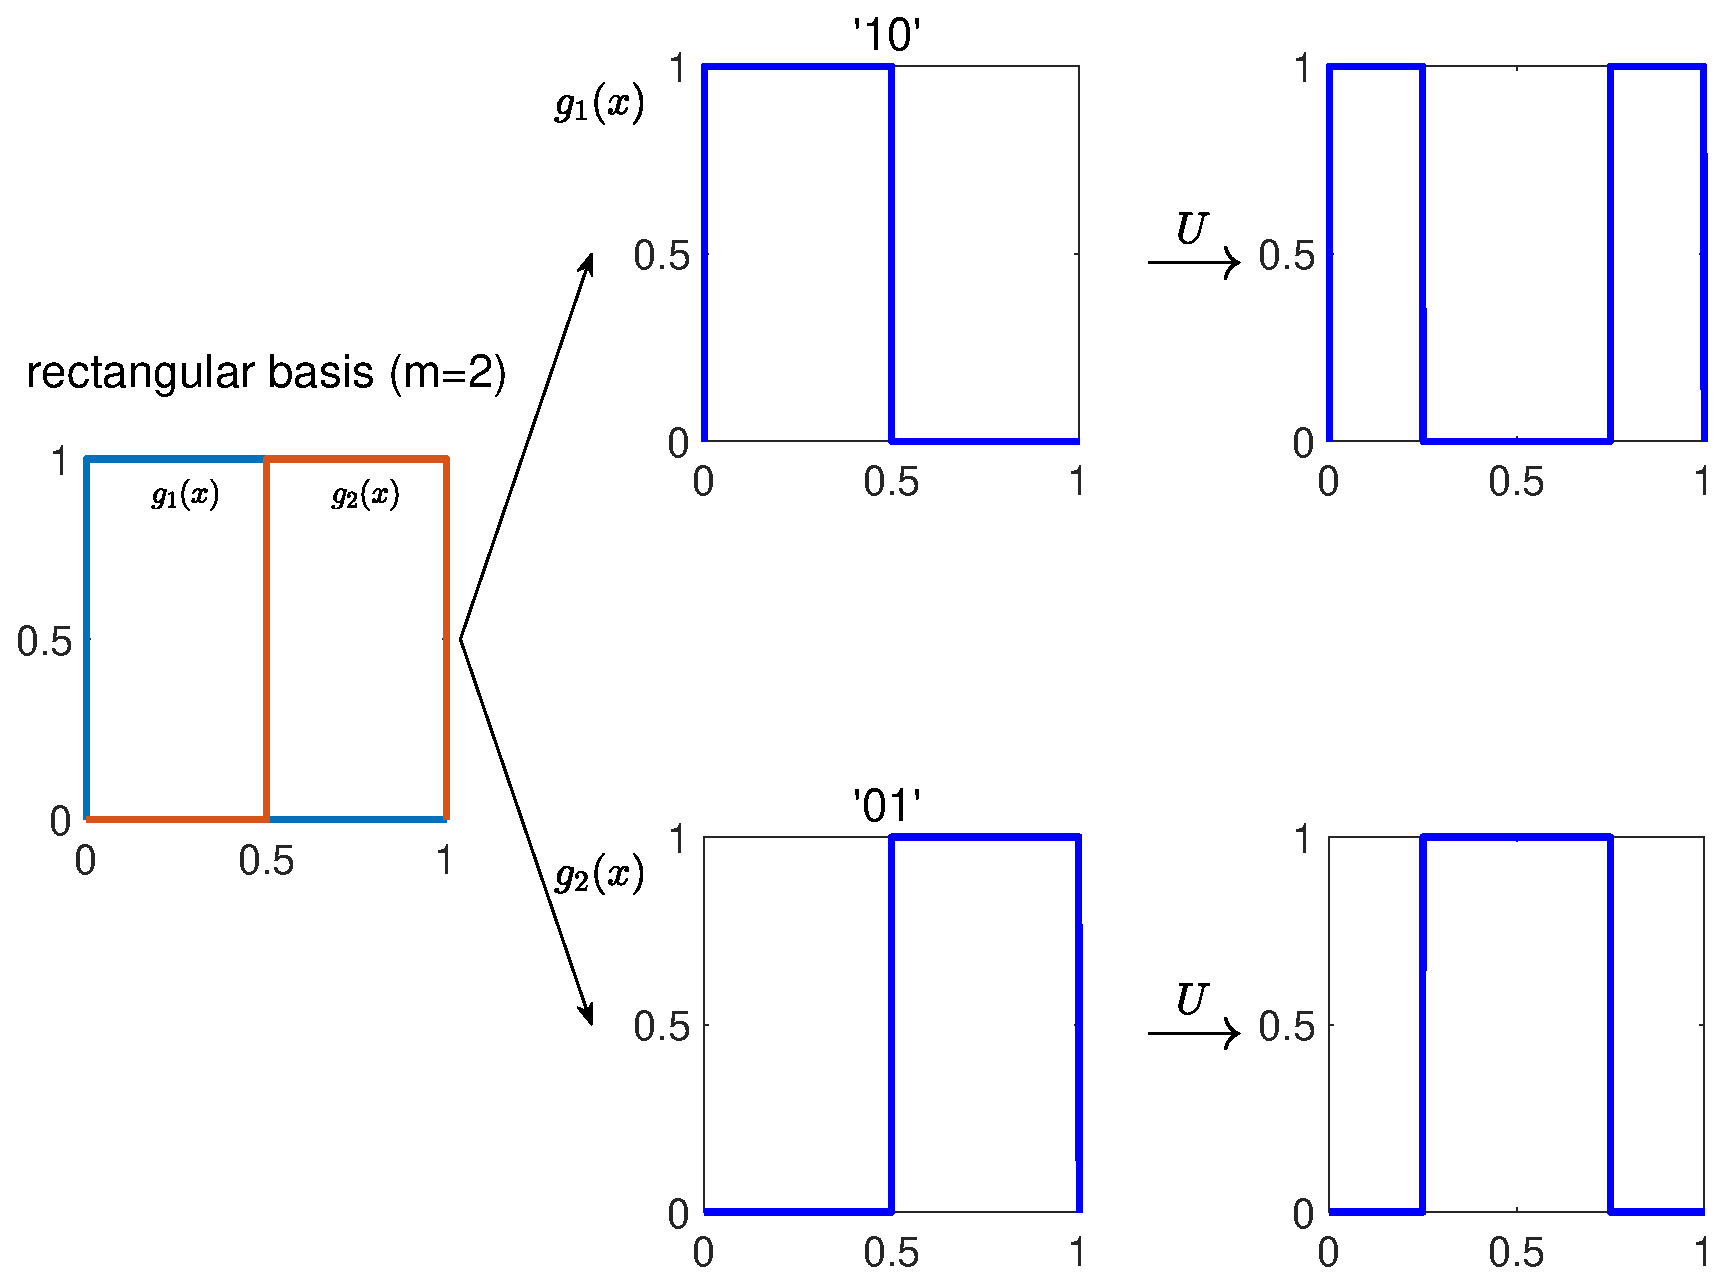
\includegraphics[width=2in]{images/01a-Tent_U2.eps}}
	     		\centerline{$m=2$}
	     	\end{minipage}
	     	\hfill
	     	\begin{minipage}{0.45\linewidth}
	     		\centerline{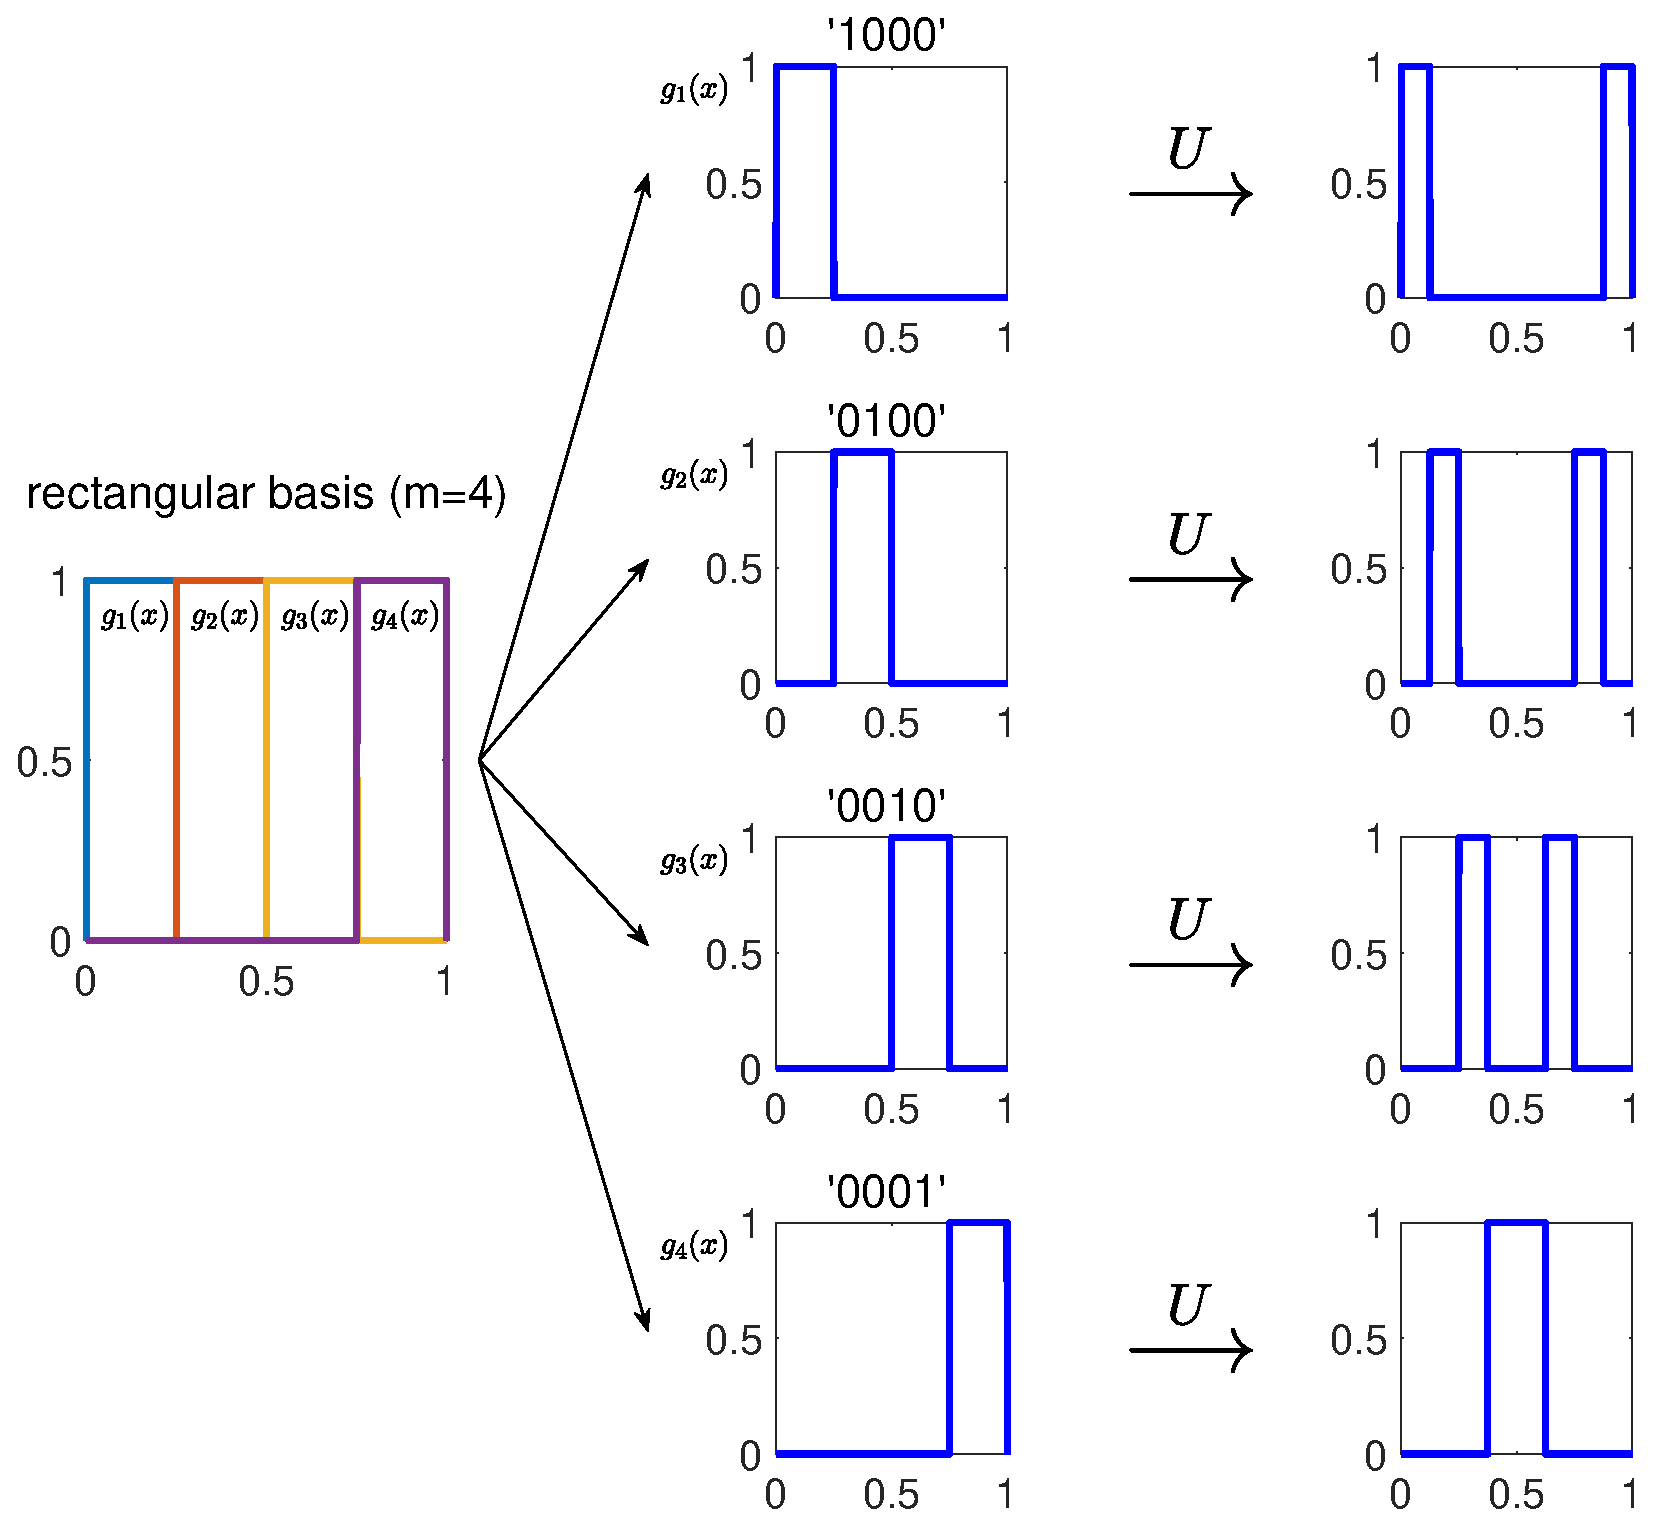
\includegraphics[width=2in]{images/01b-Tent_U4.eps}}
	     		\centerline{$m=4$}
	     	\end{minipage}
	     \end{figure}
	     \end{frame}
 
 		\begin{frame}{本征函数的数值计算-以tent map为例}
 			\begin{columns}[c]
 			\column{0.5\linewidth}
 			\begin{equation*}
 			\tilde{U}=\begin{pmatrix}
 			0.5 & 0.5 \\
 			0.5 & 0.5
 			\end{pmatrix}
 			\end{equation*}
 			\column{0.5\linewidth}
 			\begin{equation*}
 			\tilde{U}=\begin{pmatrix}
 			0.5 & 0.5 & 0 & 0 \\
 			0 & 0 & 0.5 & 0.5 \\
 			0 & 0 & 0.5 & 0.5 \\
 			0.5 & 0.5 & 0 & 0 \\
 			\end{pmatrix}
 			\end{equation*}
 		    \end{columns}
 			\begin{figure}
 				\begin{minipage}{0.45\linewidth}
 					\centerline{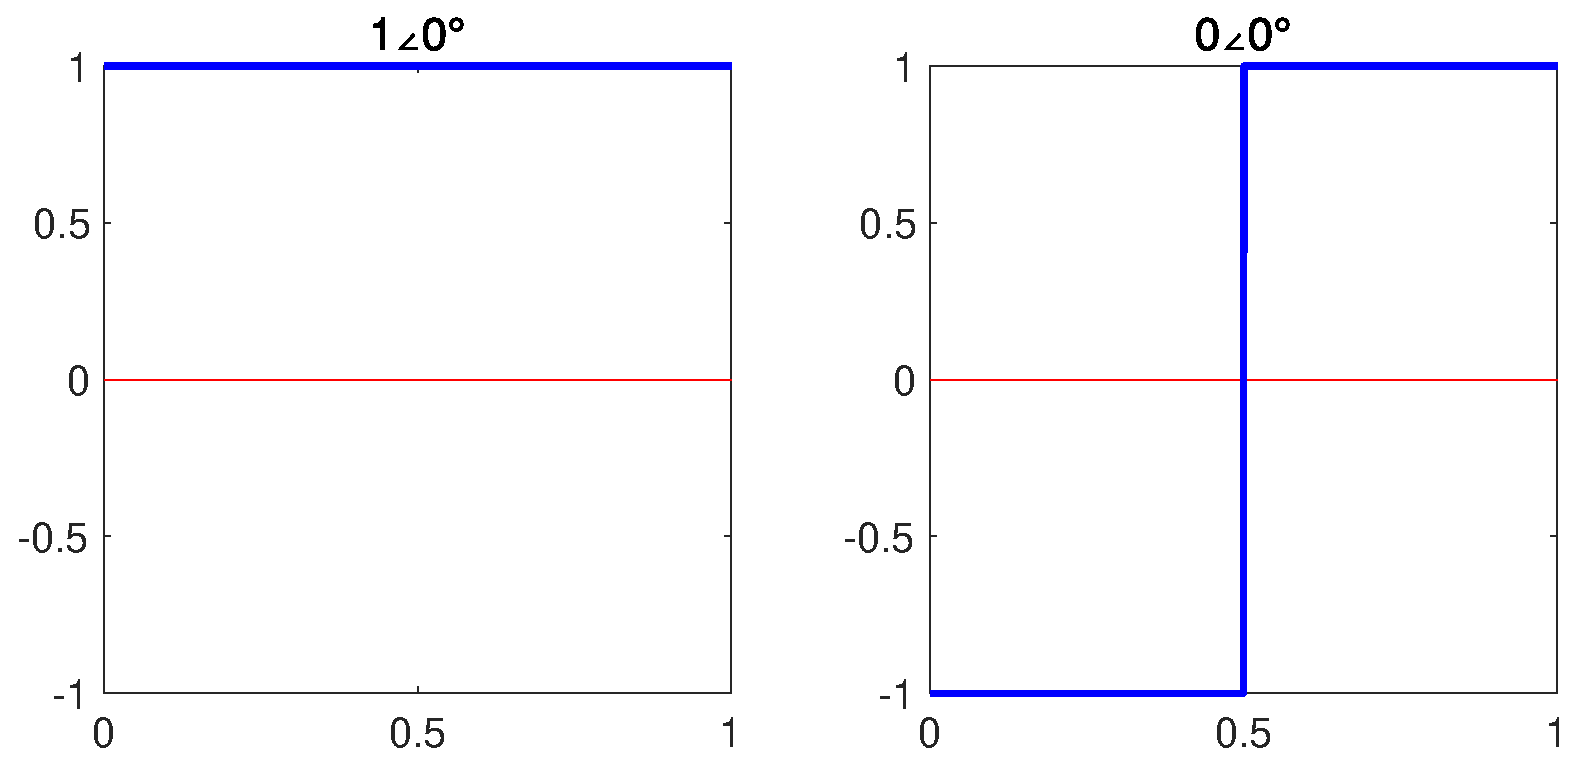
\includegraphics[width=2in]{images/02a-Koopman_eig2.eps}}
 					\centerline{$m=2$}
 				\end{minipage}
 				\hfill
 				\begin{minipage}{0.45\linewidth}
 					\centerline{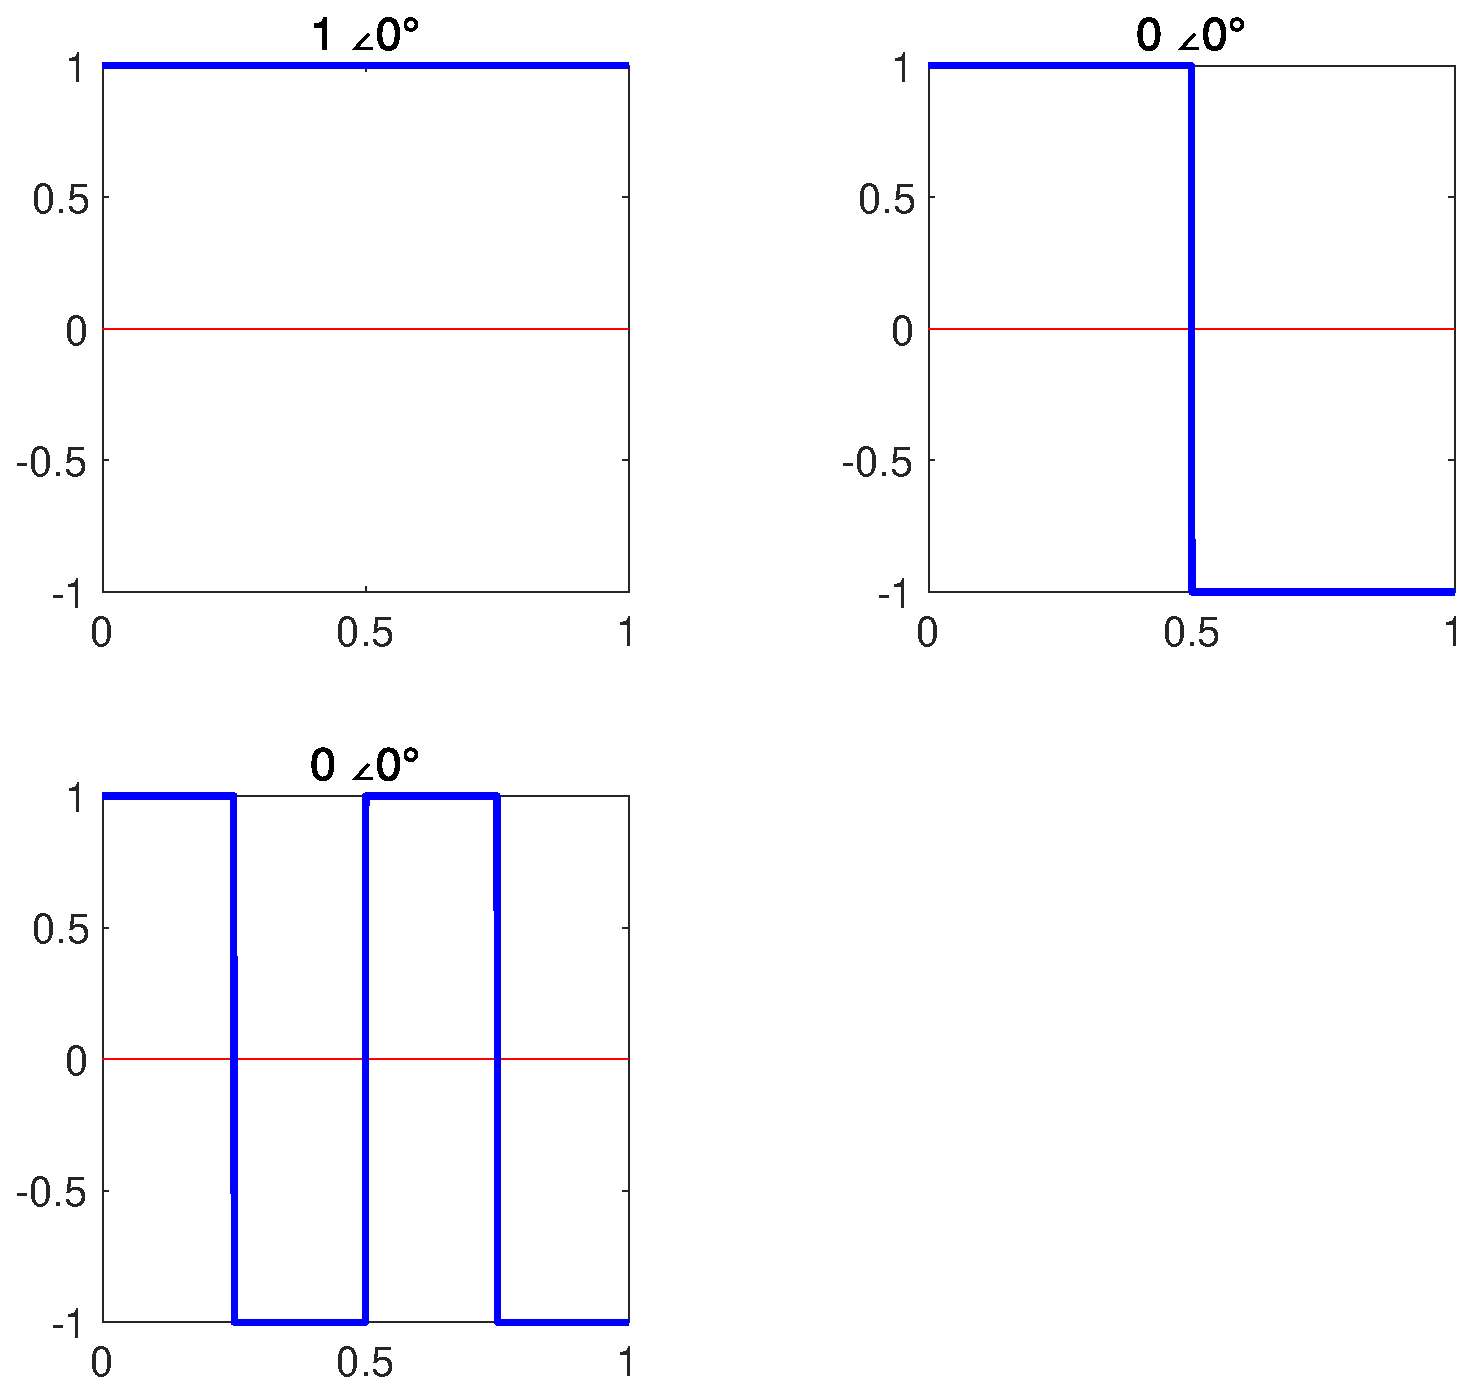
\includegraphics[width=2in]{images/02b-Koopman_eig4.eps}}
 					\centerline{$m=4$}
 				\end{minipage}
 			\end{figure}
 		\end{frame}
	\subsection{Koopman算符的函数空间}
		\begin{frame}{基函数的选取-正交基函数}
			我们需要选取一组基函数$g_1(x),g_2(x),\cdots,g_m(x)$,为了计算方便通常选择正交函数集,例如:
			\begin{example}
				\begin{align*}
				g_R(x)&=
				\begin{cases}
				1,\ &(\dfrac{i-1}{m}\leqslant x<\dfrac{i}{m})\\
				0,\ &(\mbox{otherwise})
				\end{cases},\ i=1,2,\cdots,m\\
				g_G(x)&=Cexp\left(-\dfrac{(x-x_i)^2}{2d_j^2}\right), \ x_i=\frac{i}{m}-\frac{1}{2m}\\
				g_F(x)&=e^{ik(2\pi)x},\ k=-m,-(m-1),\cdots,m-1,m\\
				g_L(x)&=\sqrt{\dfrac{2k+1}{2}}P_i(x),\ k=0,1,\cdots,m
				\end{align*}
			\end{example}
		\end{frame}
		\begin{frame}{基函数的选取-正交基函数}
			\begin{figure}
				\begin{minipage}{0.45\linewidth}
					\centerline{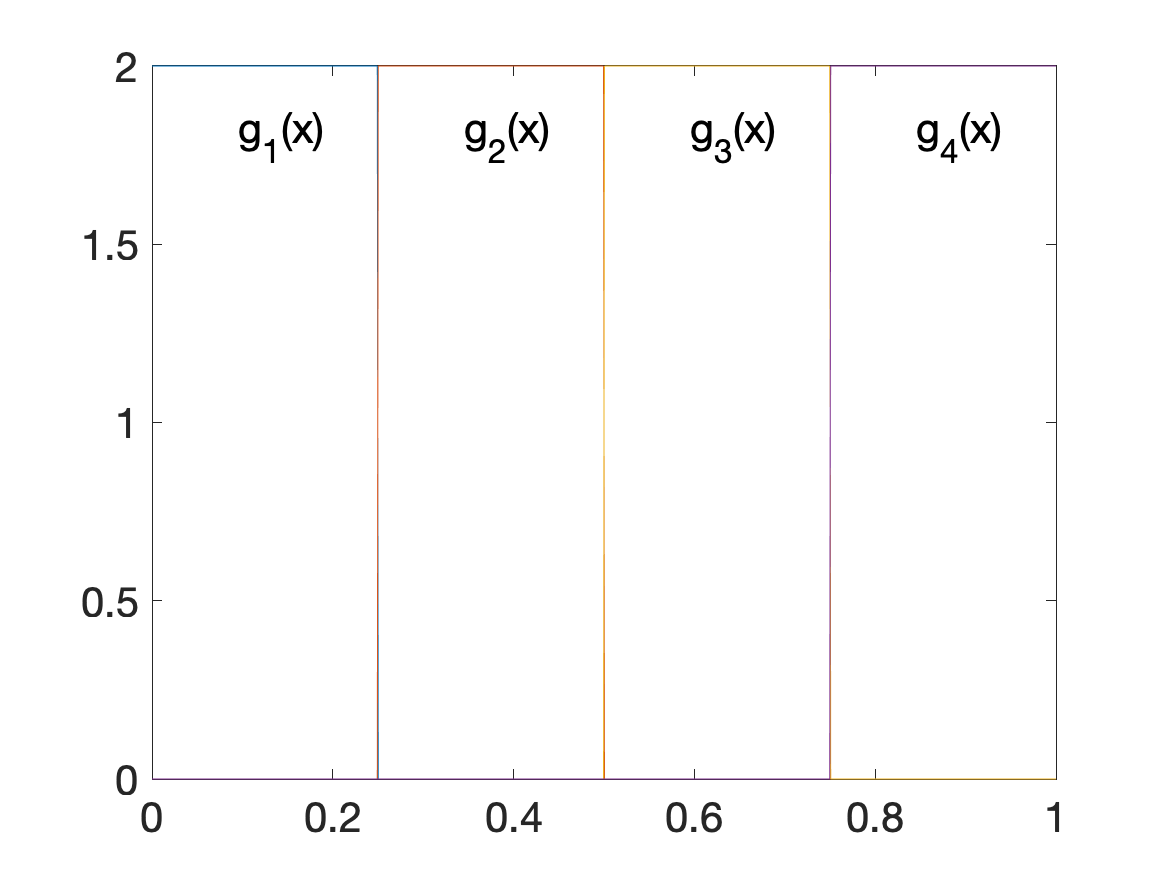
\includegraphics[width=1.7in]{images/function_basis_rect}}
					\centerline{\tiny Rectangular basis}
				\end{minipage}
			\hfill
				\begin{minipage}{0.45\linewidth}
					\centerline{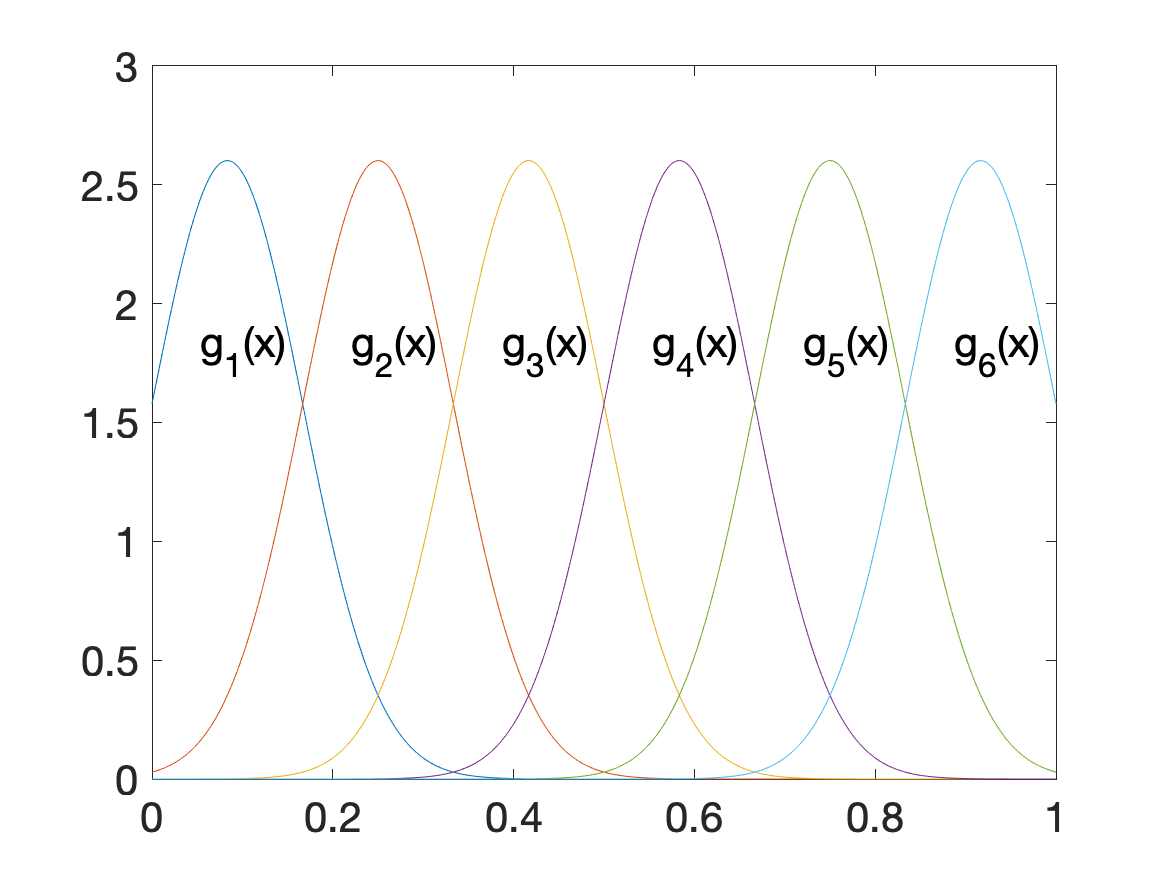
\includegraphics[width=1.7in]{images/function_basis_gauss}}
					\centerline{\tiny Gauss basis}
				\end{minipage}\\
			\begin{minipage}{0.45\linewidth}
				\centerline{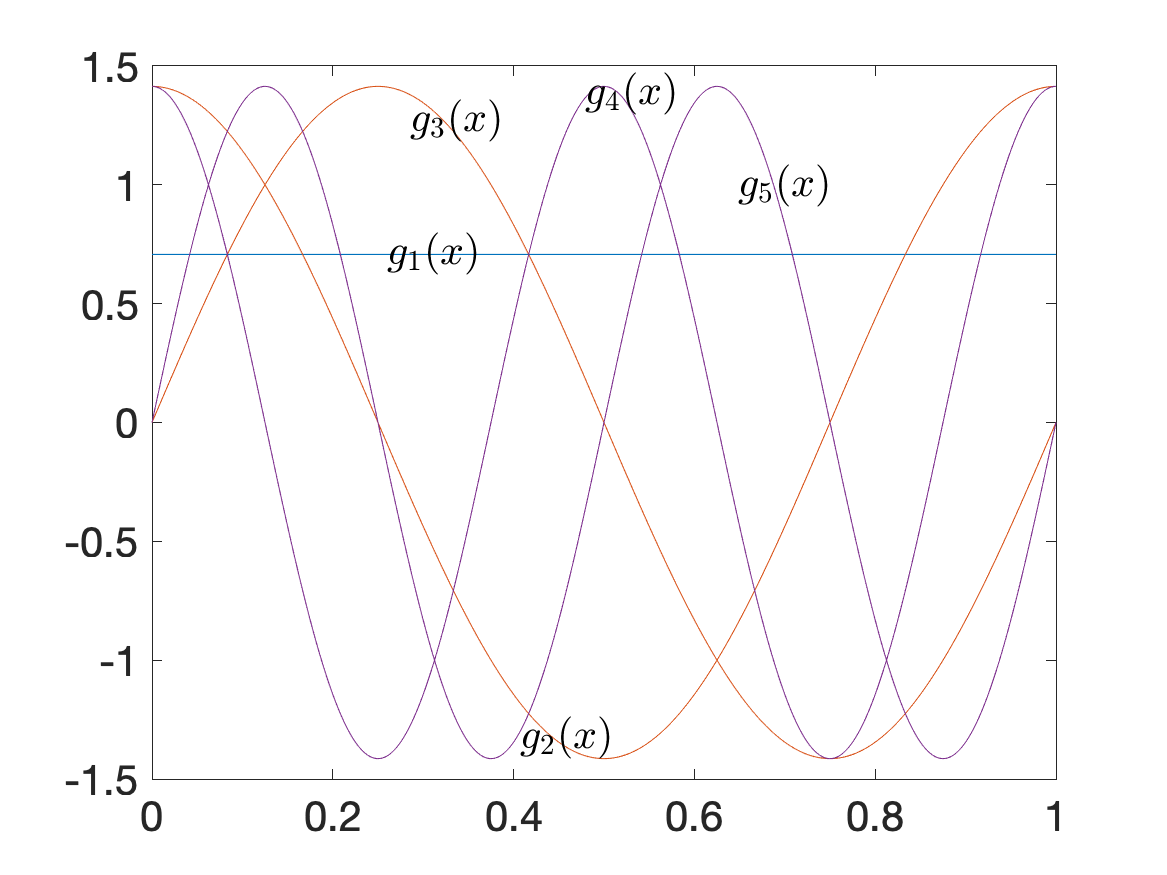
\includegraphics[width=1.7in]{images/function_basis_four}}
				\centerline{\tiny Fourier basis}
			\end{minipage}
		\hfill
			\begin{minipage}{0.45\linewidth}
				\centerline{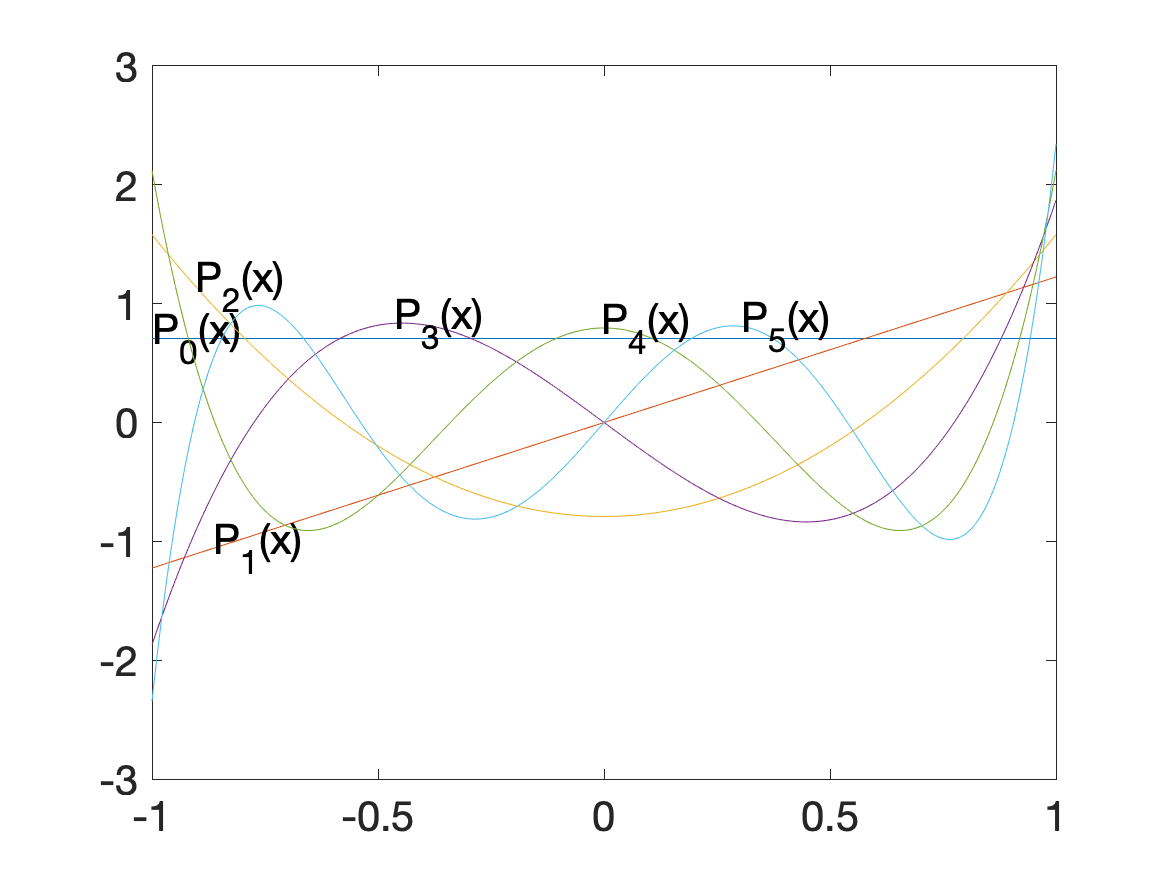
\includegraphics[width=1.7in]{images/function_basis_legen}}
				\centerline{\tiny Legendre basis}
			\end{minipage}
			\end{figure}
		\end{frame}
		\begin{frame}{基函数的选取-自然基函数}
			正交基函数可能会随着相空间的拉伸折叠,所需的基函数数量成倍增加,为此可以考虑利用从演化数据本身构建的自然基函数:
			$$g_i(x)=(x_i,x_{i+1},\cdots,x_{n+i-1})^T$$
			在Koopman算符的作用下
			\begin{equation*}
			\begin{aligned}
			Ug_i(\mathbf{x})&=U(x_i,x_{i+1},\cdots,x_{n+i-1})^T\\
			&=(x_{i+1},x_{i+2},\cdots,x_{n+i})^T\\
			&=g_{i+1}(x)
			\end{aligned}
			\end{equation*}
			Brunton等人于2017年提出了这样并排放置的基函数形成了Hankel矩阵,并通过Koopman算符描述了一步演化,即我们可以将数据矩阵$K$和$L$的关系写为
			\begin{equation*}
			\begin{pmatrix}
			x_1&x_2&\cdots&x_m\\
			x_2&x_3&\cdots&x_{m+1}\\
			\vdots&\vdots&\ddots&\vdots\\
			x_n&x_{n+1}&\cdots&x_{m+n-1}
			\end{pmatrix}
			\tilde{U}=
			\begin{pmatrix}
			x_2&x_3&\cdots&x_{m+1}\\
			x_3&x_4&\cdots&x_{m+2}\\
			\vdots&\vdots&\ddots&\vdots\\
			x_{n+1}&x_{n+2}&\cdots&x_{m+n}
			\end{pmatrix}
			\end{equation*}
		\end{frame}
	
\section{混沌系统中的Koopman算符}
	\subsubsection{一维映射:Tent Map \& Logistic Map}
		\begin{frame}{Tent Map}
			\begin{block}{动力学方程}
				$$x_{n+1}=f(x_n)=1-2|x-\frac{1}{2}|$$
				$$x_n\in [0,1], n=1,2,3,\cdots$$
			\end{block}
			两个不动点:0和$\frac{2}{3}$
			\begin{figure}
				\begin{minipage}{0.4\linewidth}
					\centering
					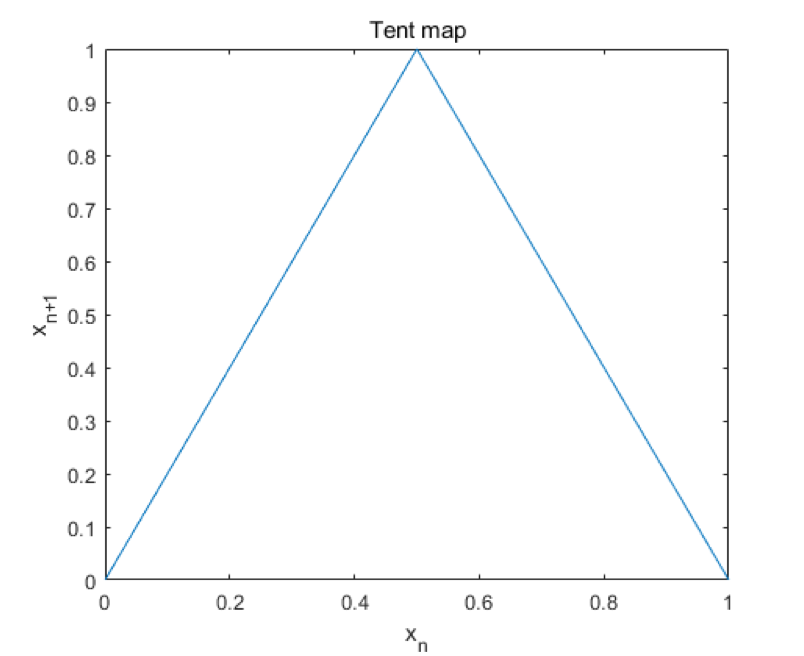
\includegraphics[width=1.8in]{figure/tent_phase}
					\caption{Tent map相图}
				\end{minipage}
			\end{figure}
		\end{frame}
		\begin{frame}{Logistic Map}
		\begin{block}{动力学方程}
			$$x_{n+1}=f(x_n)=\gamma x_n(1-x_n)$$
			$$x_n\in [0,1], n=1,2,3,\cdots$$
		\end{block}
		这里我们取$\gamma=4$,使该系统处于混沌状态。\\
		两个不动点:0和$\frac{3}{4}$。
		\begin{figure}
			\begin{minipage}{0.4\linewidth}
				\centering
				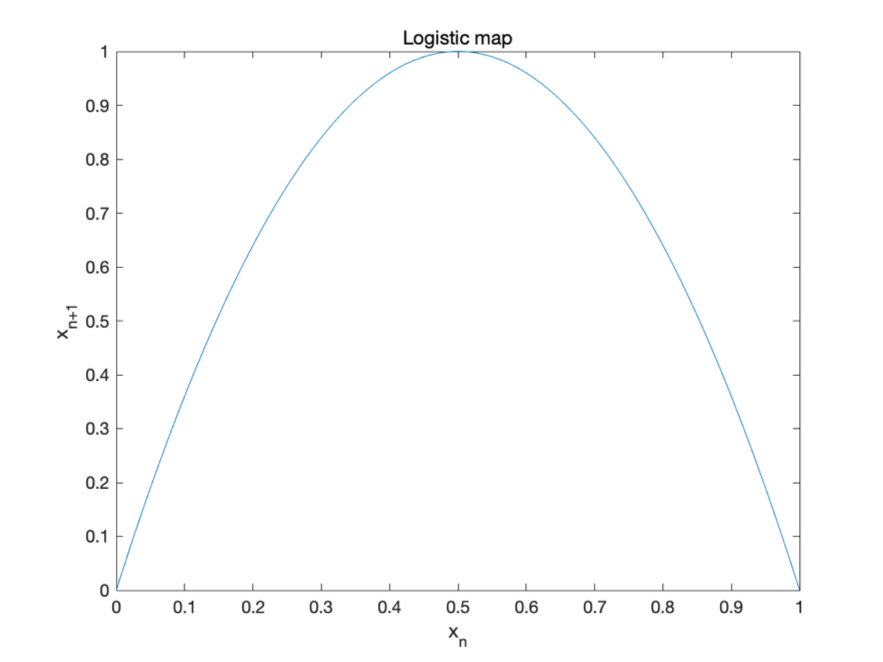
\includegraphics[width=1.8in]{figure/logistic_phase}
				\caption{Logistic map相图}
			\end{minipage}
			\begin{minipage}{0.4\linewidth}
				\centering
				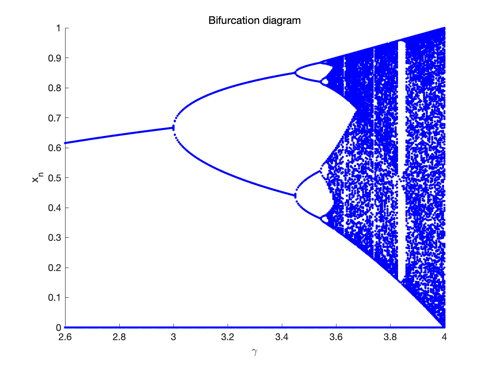
\includegraphics[width=1.8in]{figure/logistic_bifurcation}
				\caption{Logistic map分岔图}
			\end{minipage}
		\end{figure}
		\end{frame}
		\begin{frame}{Logistic-动力学过程}
			\centering
			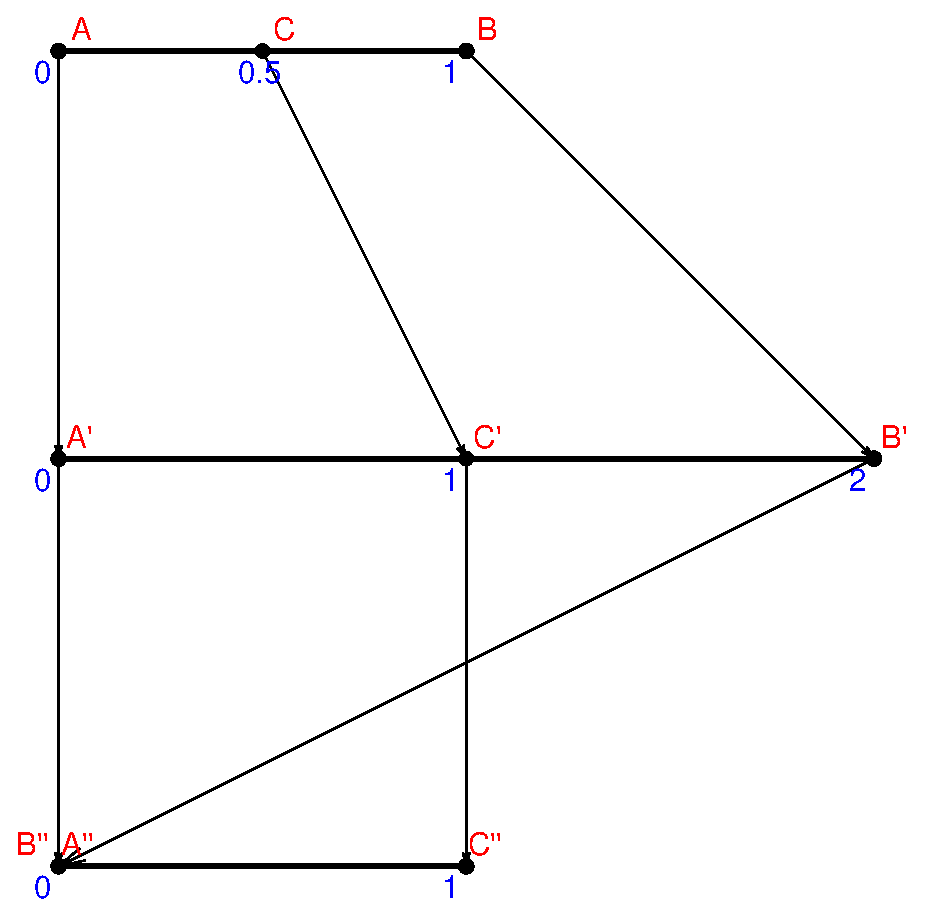
\includegraphics[width=3in]{images/Logistic_dynamic}
		\end{frame}
      \begin{frame}{Logistic-符号动力学划分}
      	\centering
      	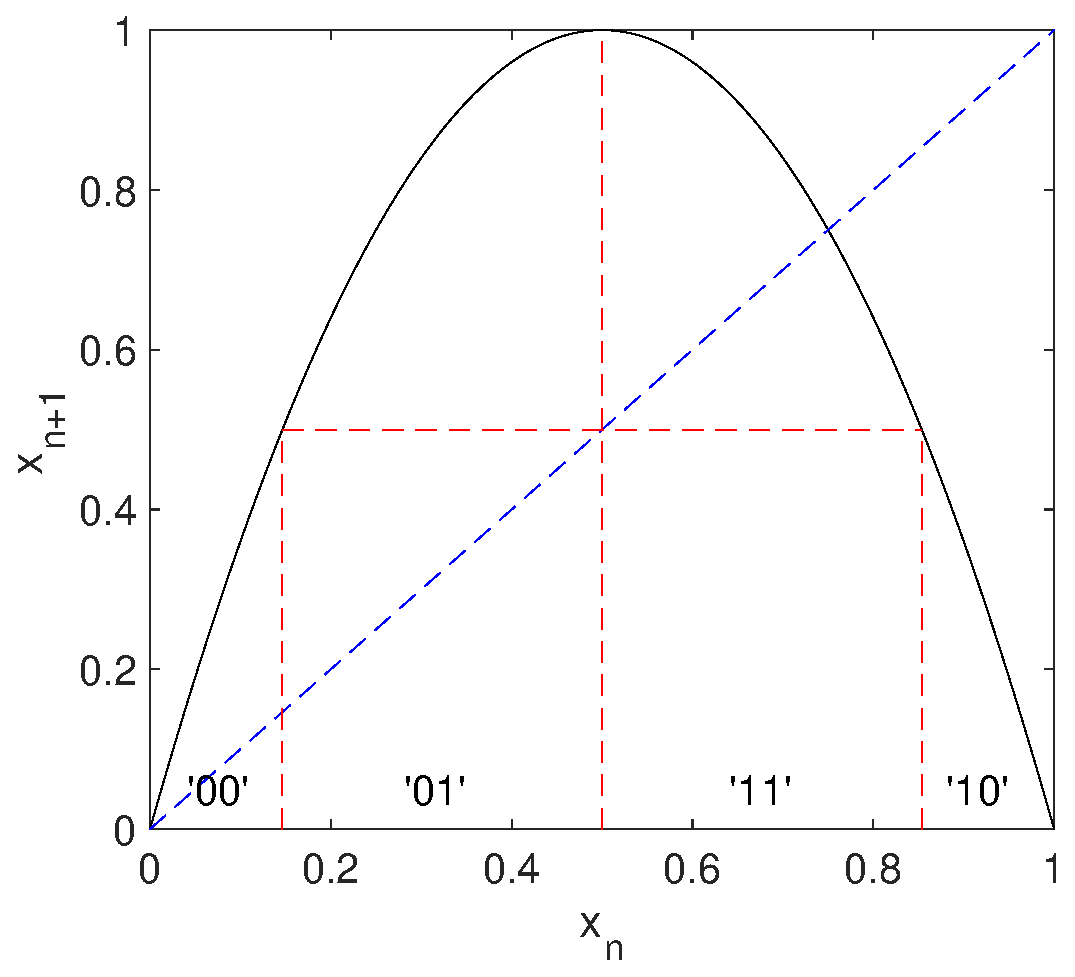
\includegraphics[width=3in]{images/02c-Logistic_symbolic}
      \end{frame}
      \begin{frame}
      	\begin{figure}
      		\begin{minipage}{0.9\linewidth}
      			\centerline{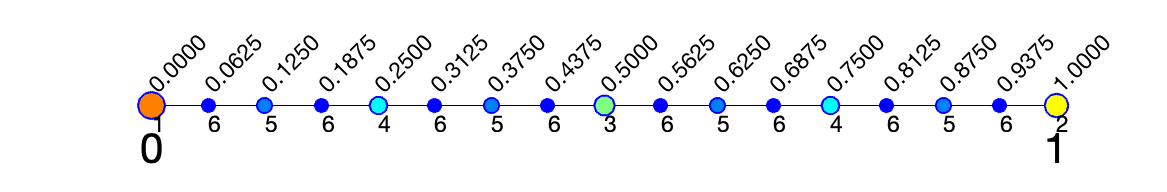
\includegraphics[width=4.2in]{images/Tent_boundary.png}}
      			\centerline{tent map}
      		\end{minipage}
      		\\
      		\begin{minipage}{0.9\linewidth}
      			\centerline{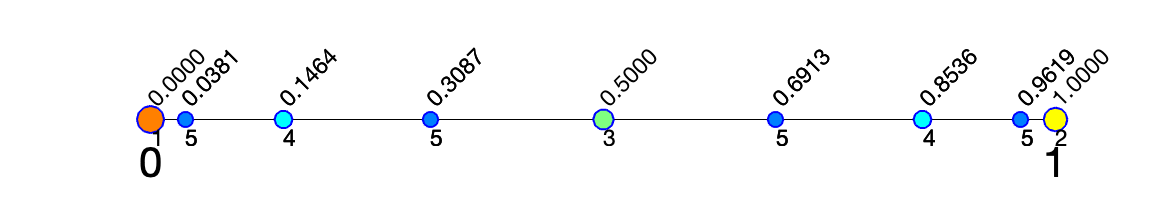
\includegraphics[width=4.2in]{images/Logistic_boundary.png}}
      			\centerline{logistic map}
      		\end{minipage}
      	\end{figure}
      \end{frame}
      \begin{frame}{Gauss基函数下的本征函数}
      	\begin{figure}
      		\begin{minipage}{0.45\linewidth}
      			\centerline{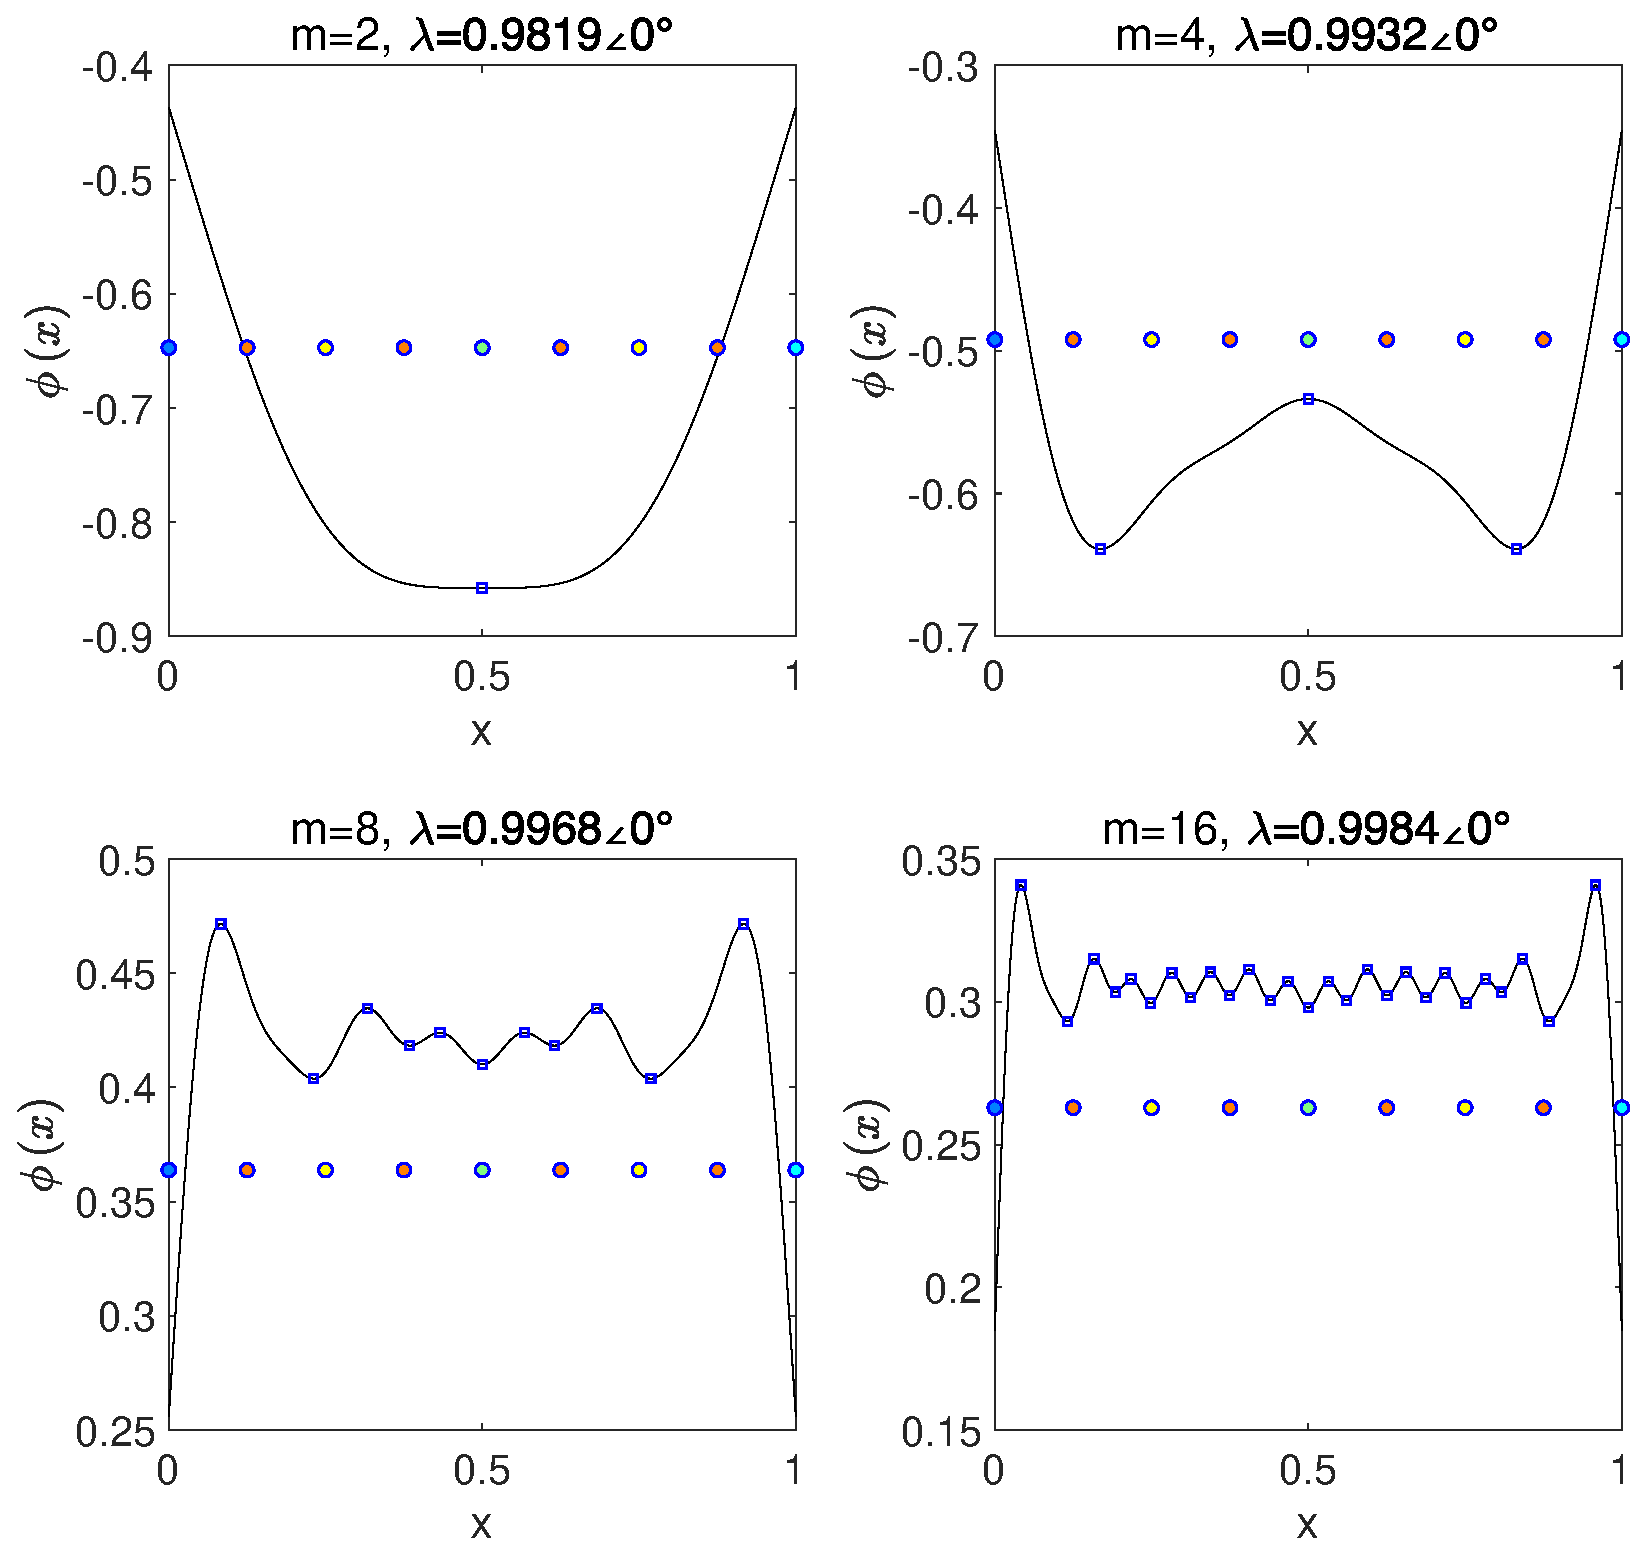
\includegraphics[width=2.2in]{images/03a-Tent_eigen_Gauss_n1000_m2-4-8-16_d0.eps}}
      			\centerline{tent map}
      		\end{minipage}
      		\hfill
      		\begin{minipage}{0.45\linewidth}
      			\centerline{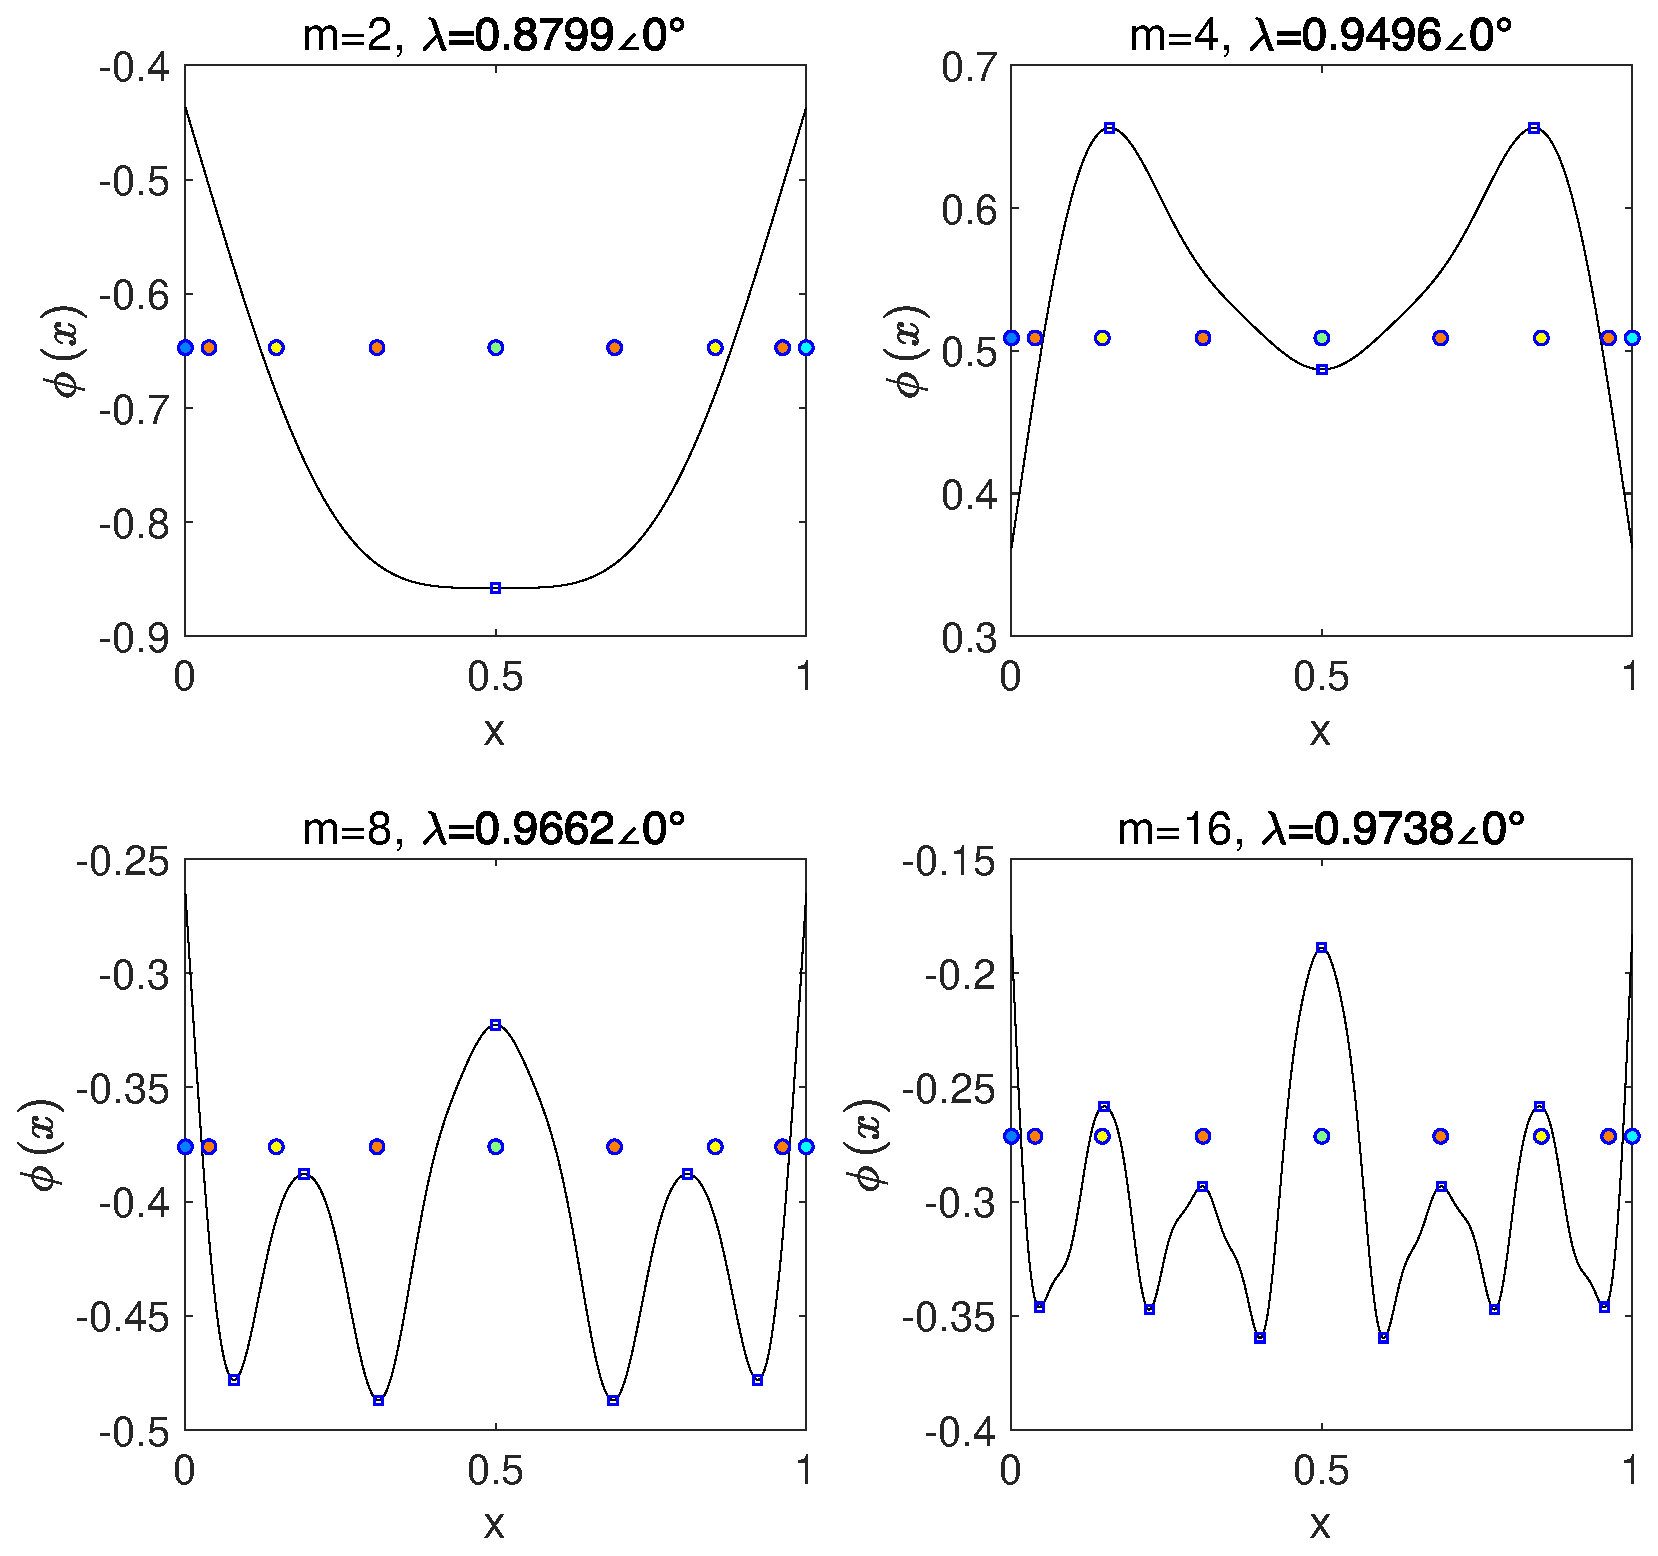
\includegraphics[width=2.2in]{images/03b-Logistic_eigen_Gauss_n1000_m2-4-8-16_d0.eps}}
      			\centerline{logistic map}
      		\end{minipage}
       \end{figure}
      \end{frame}
      \begin{frame}{自然基函数下的本征函数}
      	\begin{figure}
      		\begin{minipage}{0.45\linewidth}
      			\centerline{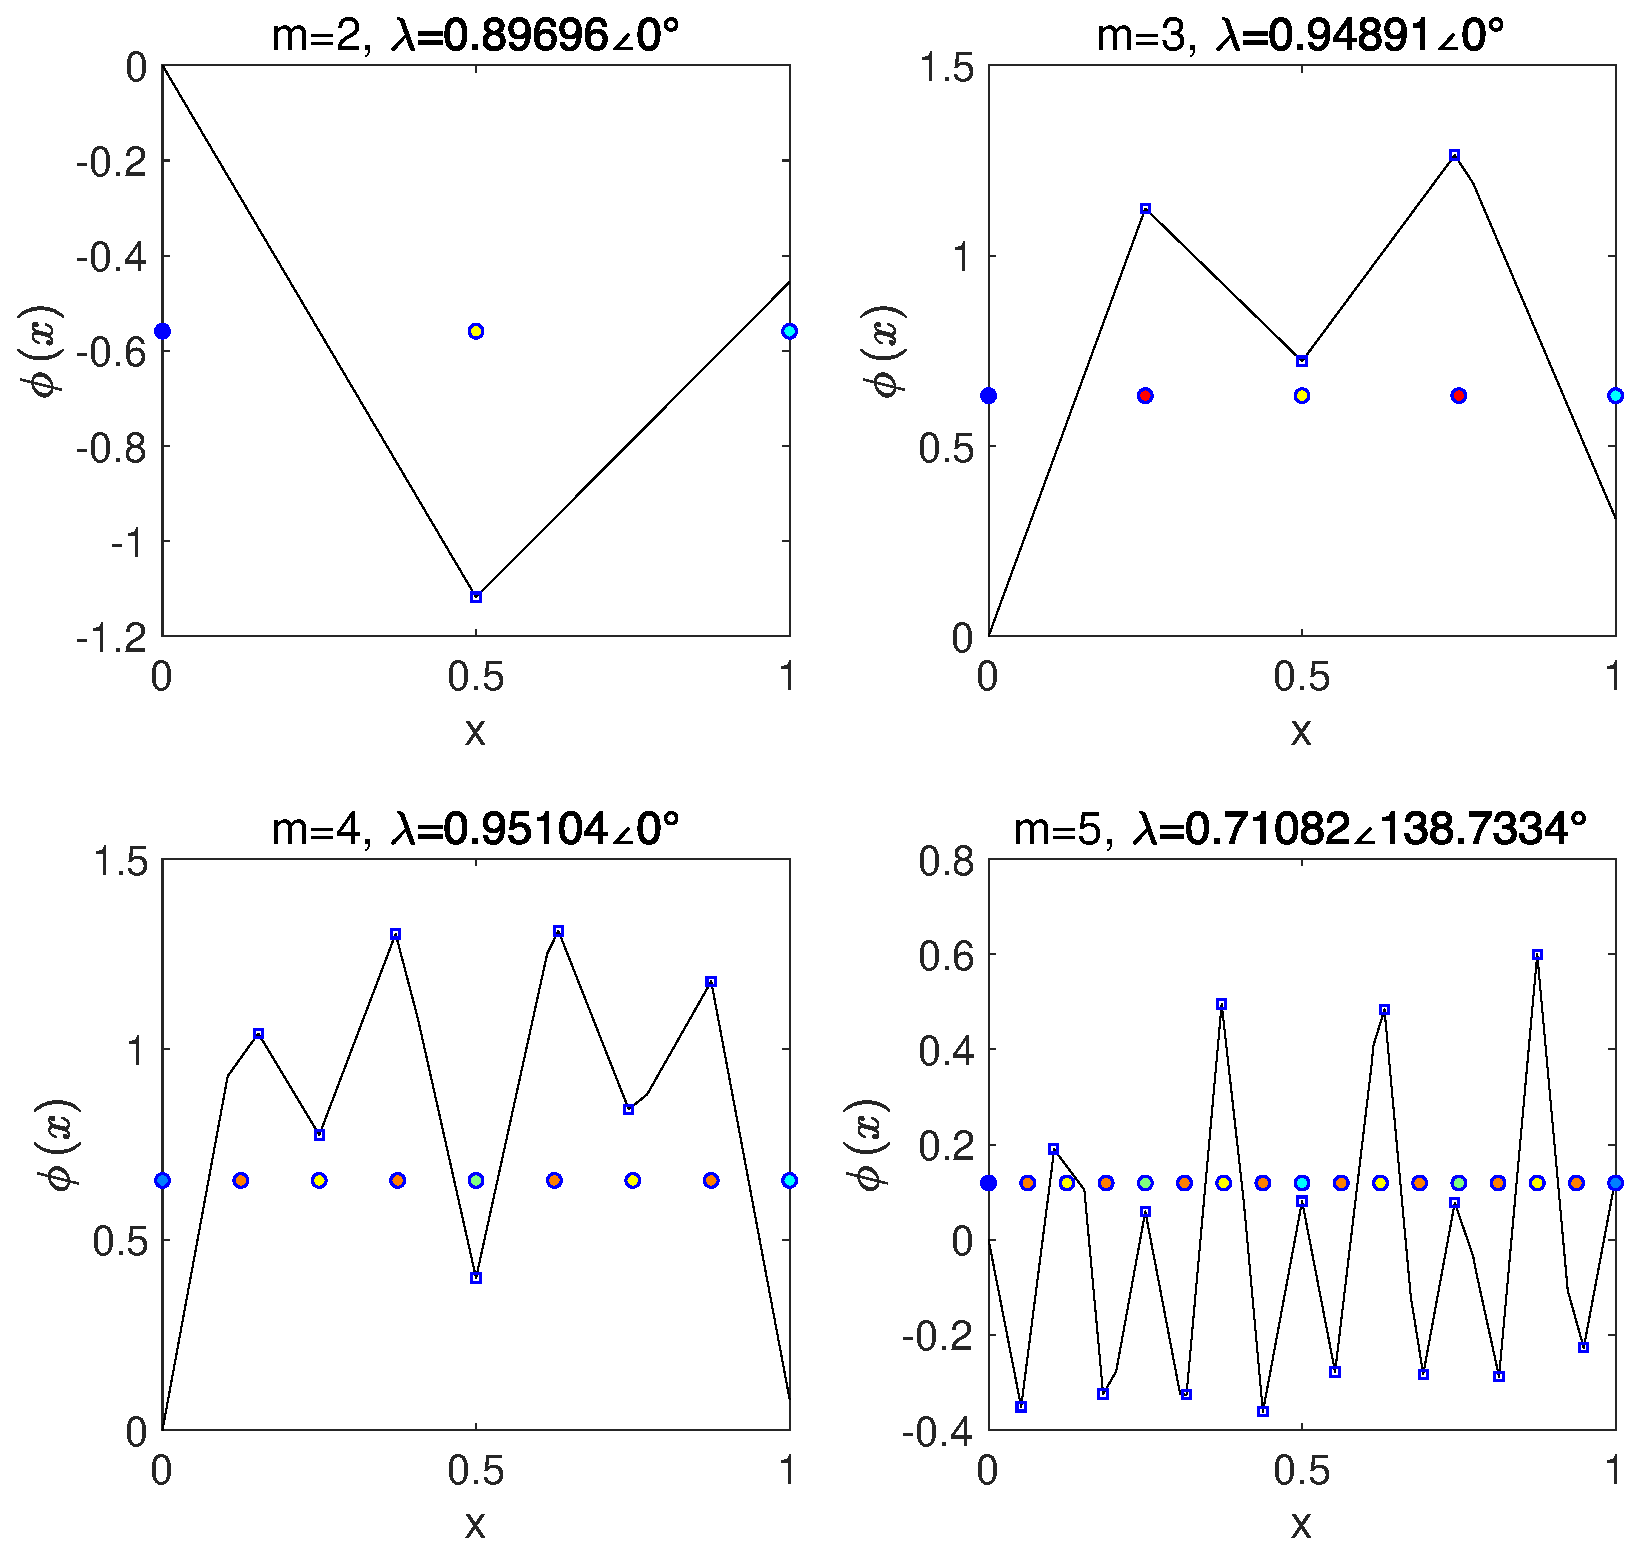
\includegraphics[width=2.2in]{images/04a-Tent_eigen_natural_n1000_m2-3-4-5.eps}}
      			\centerline{tent map}
      		\end{minipage}
      		\hfill
      		\begin{minipage}{0.45\linewidth}
      			\centerline{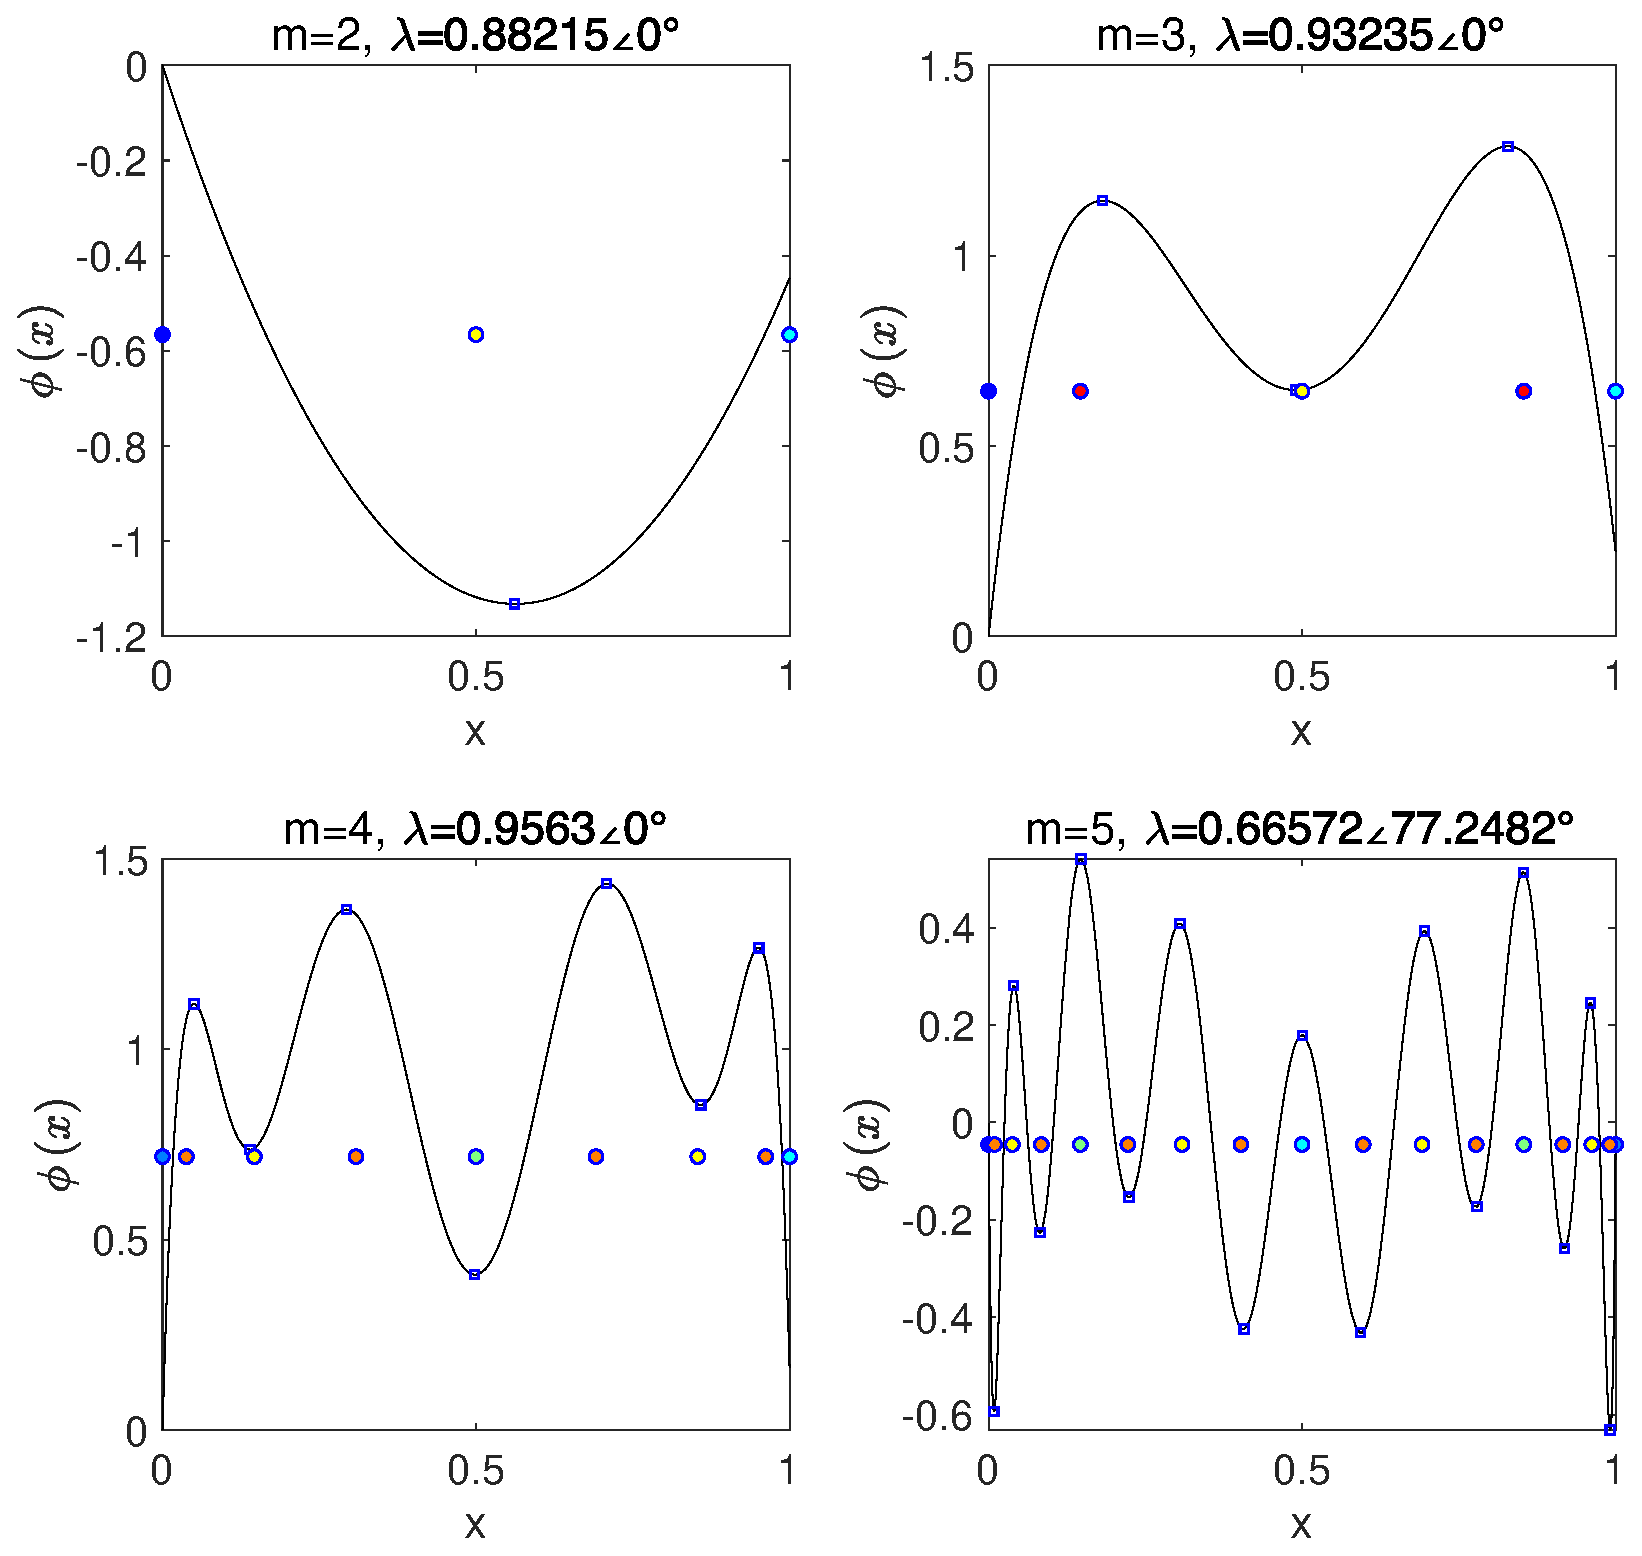
\includegraphics[width=2.2in]{images/04b-Logistic_eigen_natural_n1000_m2-3-4-5.eps}}
      			\centerline{logistic map}
      		\end{minipage}
      	\end{figure}
      \end{frame}
	\begin{frame}
		\scriptsize \centering
		\begin{tabular}{cccccc}
			\multirow{2}{*}{$m$}
			&\multirow{2}{*}{$l$}
			&\multicolumn{2}{c}{tent map}
			&\multicolumn{2}{c}{logistic map}\\ \cline{3-6}
			&&\textrm{extremum}&\textrm{boundary}&\textrm{extremum}&\textrm{boundary}\\
			\hline
			\multirow{1}{*}{$2$}& \multirow{1}{*}{$0$} & 0.5000 & 0.5000 & 0.5585 & 0.5000\\
			\hline
			\multirow{3}{*}{$3$}& \multirow{1}{*}{$0$} & 0.5000 & 0.5000 & 0.4868 & 0.5000\\ \cline{2-6}
			& \multirow{2}{*}{$1$} & 0.2502 & 0.2500 & 0.1847 & 0.1464\\
			& & 0.7500 & 0.7500 & 0.8299 & 0.8536\\
			\hline
			\multirow{7}{*}{$4$}& \multirow{1}{*}{$0$} & 0.5000 & 0.5000 & 0.4972 & 0.5000\\ \cline{2-6}
			& \multirow{2}{*}{$1$} & 0.2503 & 0.2500 & 0.1378 & 0.1464\\
			& & 0.7500 & 0.7500 & 0.8602 & 0.8536\\ \cline{2-6}
			& \multirow{4}{*}{$2$} & 0.1305 & 0.1250 & 0.0518 & 0.0381\\
			& & 0.3750 & 0.3750 & 0.2938 & 0.3087\\
			& & 0.6191 & 0.6250 & 0.7107 & 0.6913\\
			& & 0.8749 & 0.8750 & 0.9485 & 0.9619\\
			\hline
			\multirow{15}{*}{$5$}& \multirow{1}{*}{$0$} & 0.5000 & 0.5000 & 0.4995 & 0.5000\\ \cline{2-6}
			& \multirow{2}{*}{$1$} & 0.2500 & 0.2500 & 0.1472 & 0.1464\\
			& & 0.7443 & 0.7500 & 0.8522& 0.8536\\ \cline{2-6}
			& \multirow{4}{*}{$2$} & 0.1195 & 0.1250 & 0.0402 & 0.0381\\
			& & 0.3787 & 0.3750 & 0.3024 & 0.3087\\
			& & 0.6278 & 0.6250 & 0.6943 & 0.6913\\
			& & 0.8750 & 0.8750 & 0.9594 & 0.9619\\ \cline{2-6}
			& \multirow{8}{*}{$3$} & 0.0597 & 0.0625 & 0.0087 & 0.0096\\
			& & 0.1894 & 0.1875 & 0.0818 & 0.0842\\
			& & 0.3033 & 0.3125 & 0.2226 & 0.2222\\
			& & 0.4268 & 0.4375 & 0.4055 &0.4024\\
			& & 0.5625 & 0.5625 & 0.5942 & 0.5975\\
			& & 0.6861 & 0.6875 & 0.7764 & 0.7778\\
			& & 0.8172 & 0.8125 & 0.9182 & 0.9157\\
			& & 0.9560 & 0.9375 & 0.9912 & 0.9904\\
			\hline
		\end{tabular}
	\end{frame}
    \begin{frame}{一维映射-边界点划分的鲁棒性}
    	\begin{block}{高斯白噪声下的一维映射}
    		$$x_{n+1}=f(x_n)+\xi$$
    	\end{block}
    \begin{figure}
    	\begin{minipage}{0.45\linewidth}
    		\centerline{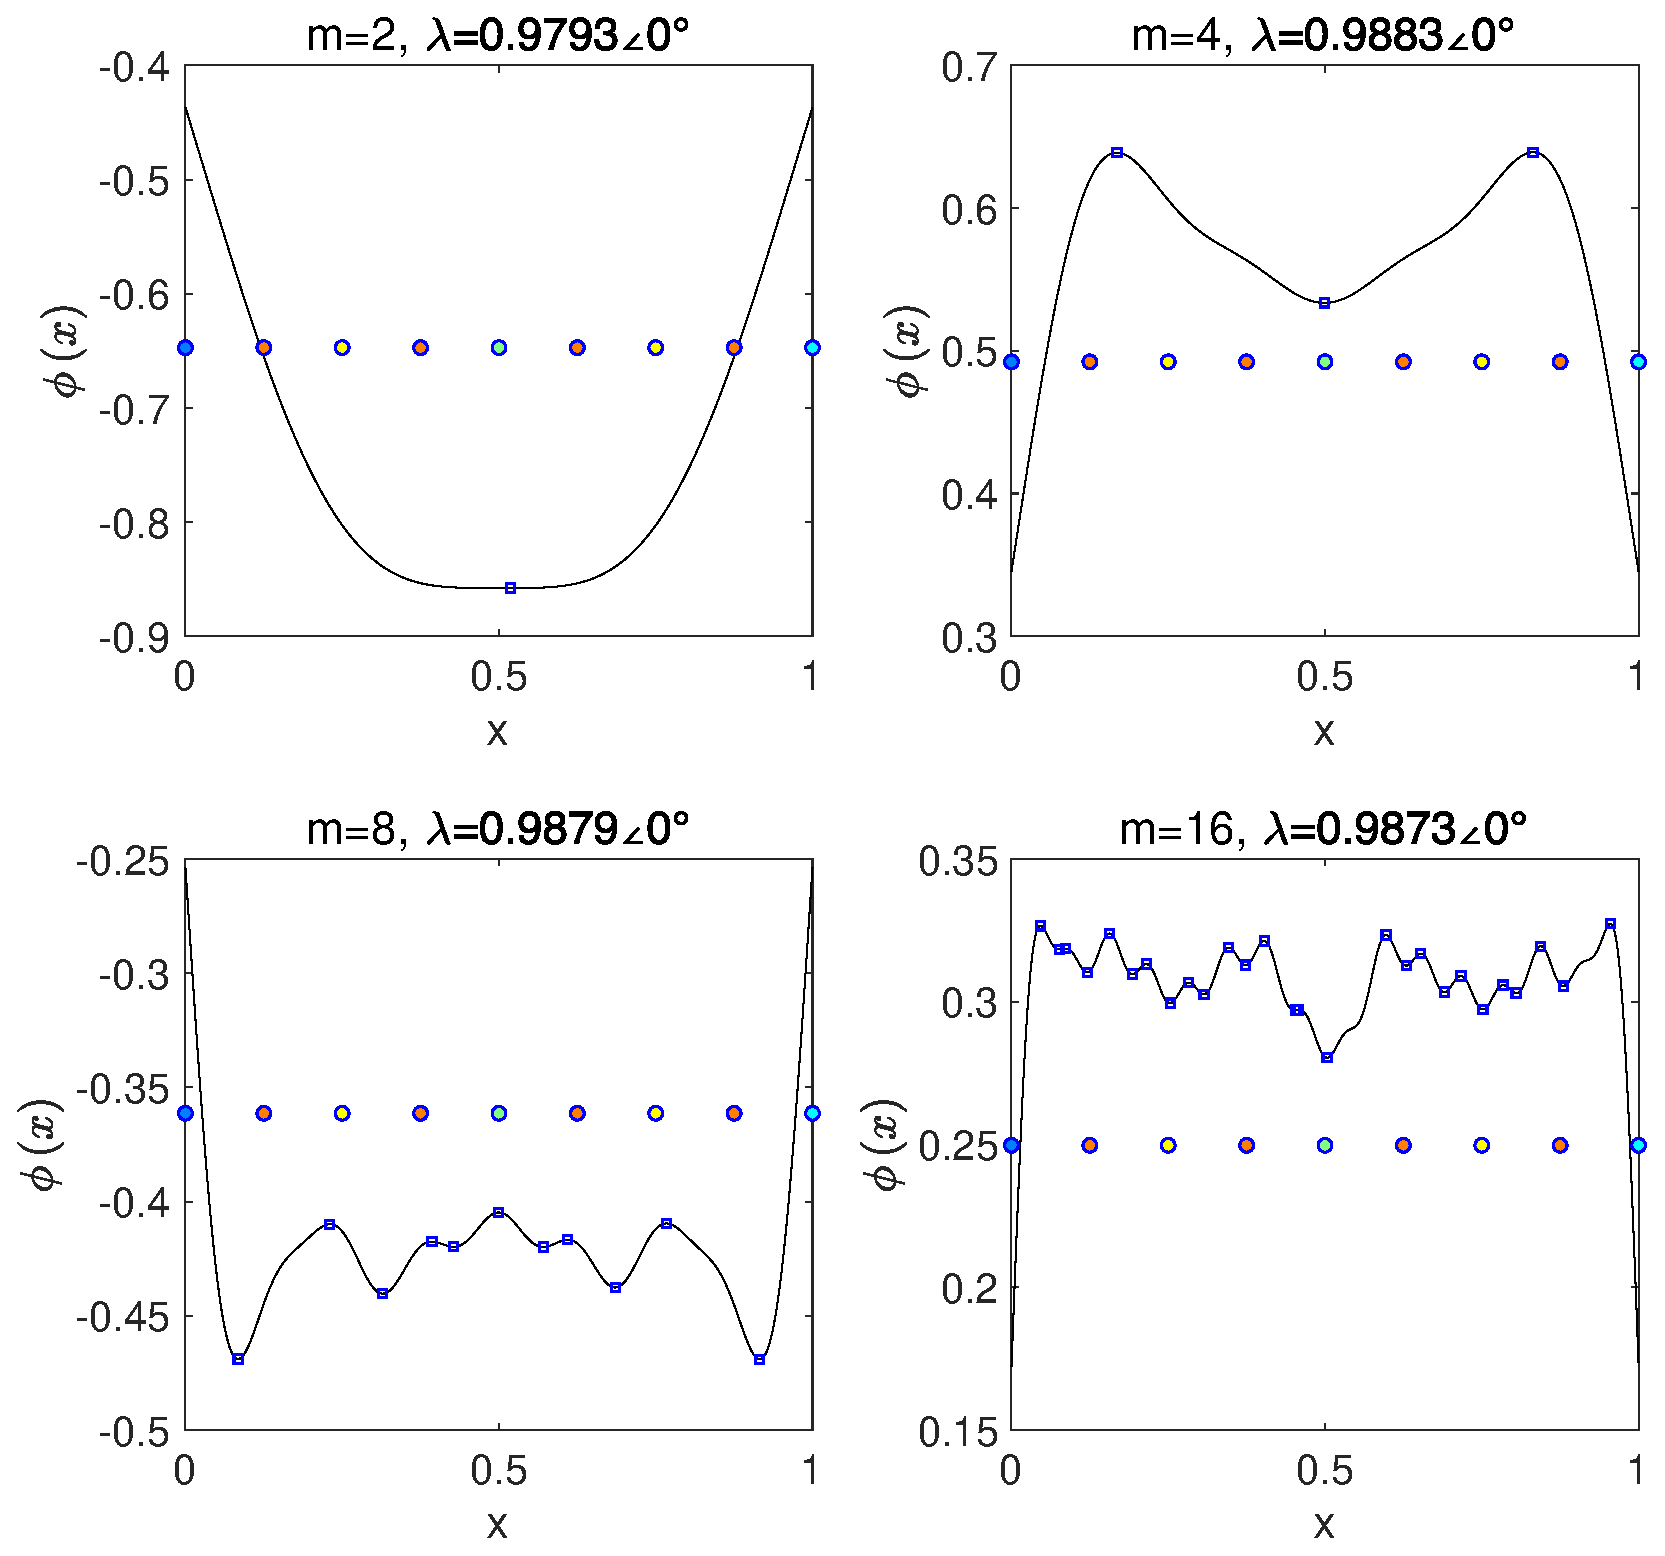
\includegraphics[width=2in]{images/05a-Tent_eigen_Gauss_n1000_m2-4-8-16_d0-001.eps}}
    		\centerline{tent map}
    	\end{minipage}
    	\hfill
    	\begin{minipage}{0.45\linewidth}
    		\centerline{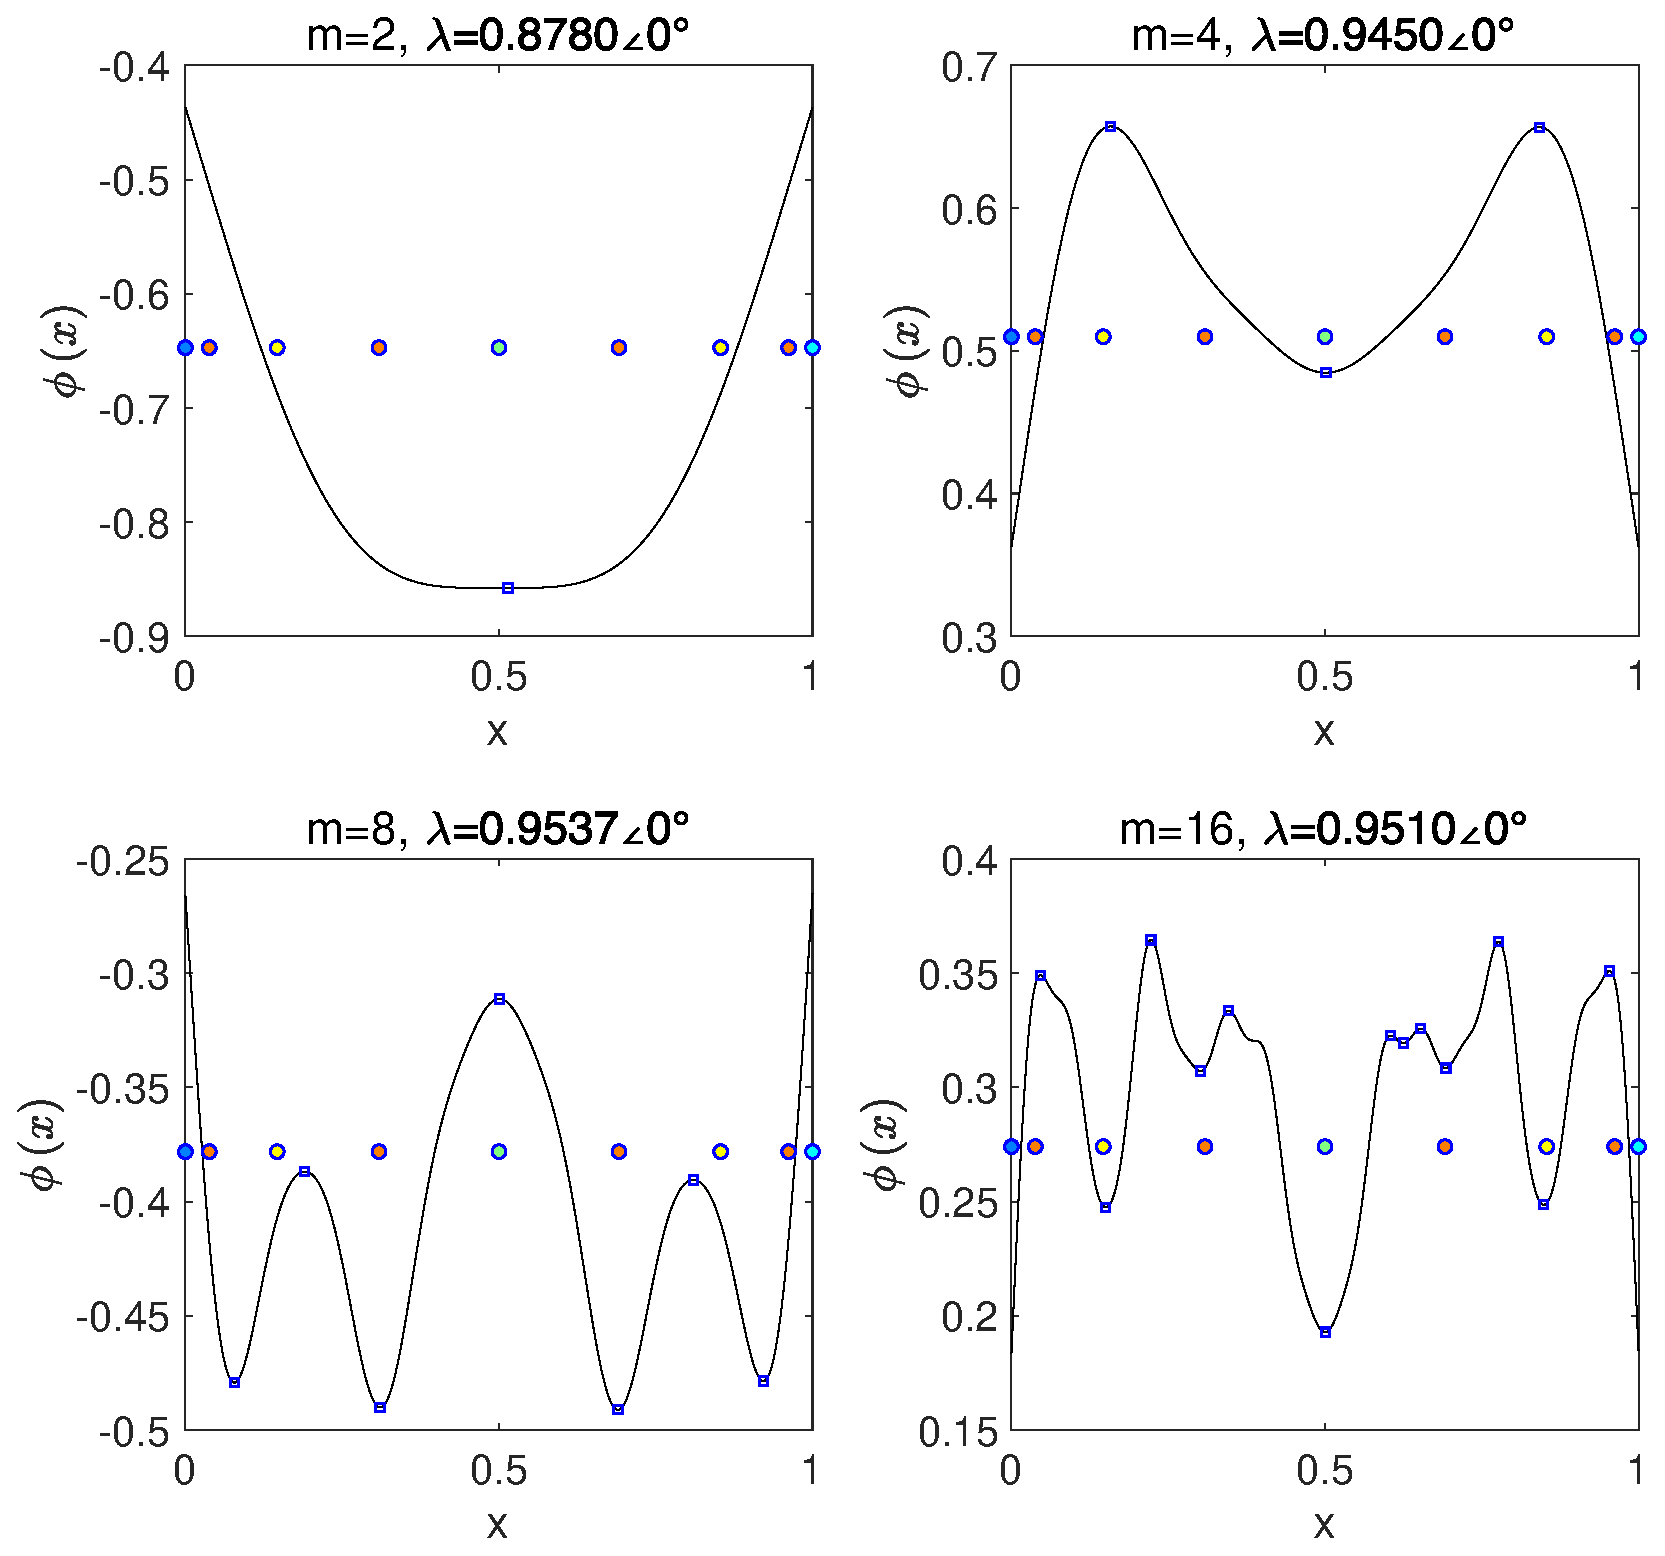
\includegraphics[width=2in]{images/05b-Logistic_eigen_Gauss_n1000_m2-4-8-16_d0-001.eps}}
    		\centerline{logistic map}
    	\end{minipage}
    \end{figure}
    \end{frame}
	\begin{frame}{一维映射-不同基函数数量之间的关系}
		随着基函数数量$m$的增加,本征函数对边界点的描述也越来越精细。为了验证此结论,我们比较基函数数量加倍时本征函数极值点之间的关系,为了比较动力学特征的相似性,我们定义本征函数的相关系数
		$$\rho(\phi_1,\phi_2)=\dfrac{\sum_i(\phi_{1i}-\overline{\phi}_1)(\phi_{2i}-\overline{\phi}_2)}{\sqrt{(\sum_i(\phi_{1i}-\overline{\phi}_1)^2)(\sum_i(\phi_{2i}-\overline{\phi}_2)^2)}}$$
		为了确定不同基函数数量$m$下本征函数的一致性,我们使用下述参数极小值的计算:
		$$\mathop{\arg\min}_{\boldsymbol{\phi_{m_2}}} \ \ || U\phi_{m_2}-\lambda \phi_{m_2} || + \mu |\rho(\phi_{m_1},\phi_{m_2})|$$
		第一项表示本征函数的定义,第二项表示相关系数,$\mu$表示权重,一般来讲,我们应保证本征函数的正确性,即通常有$\mu\ll 1$。
    \end{frame}
	\begin{frame}{一维映射-不同基函数数量之间的关系}
		\begin{figure}
			\begin{minipage}{0.45\linewidth}
				\centerline{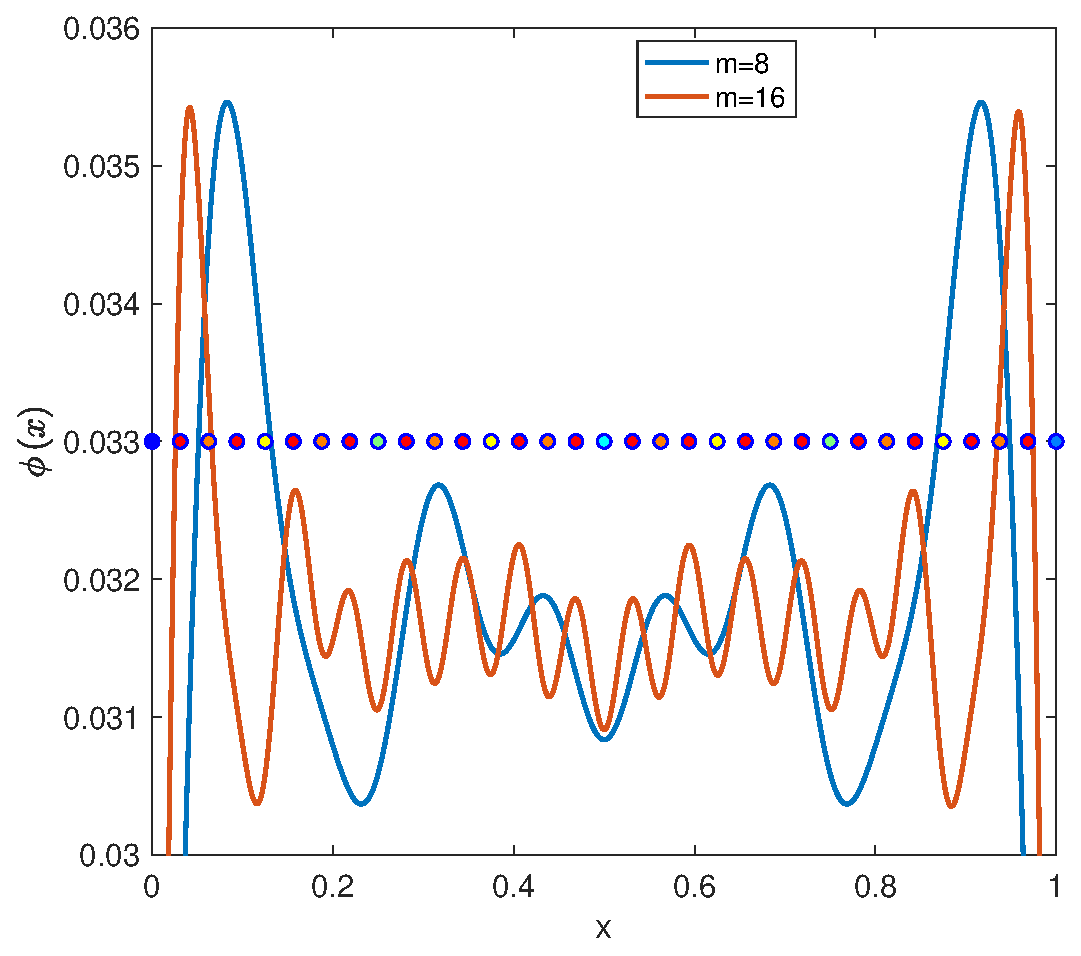
\includegraphics[width=2.2in]{images/06a-Tent_findeigen_m8m16.eps}}
				\centerline{tent map}
			\end{minipage}
			\hfill
			\begin{minipage}{0.45\linewidth}
				\centerline{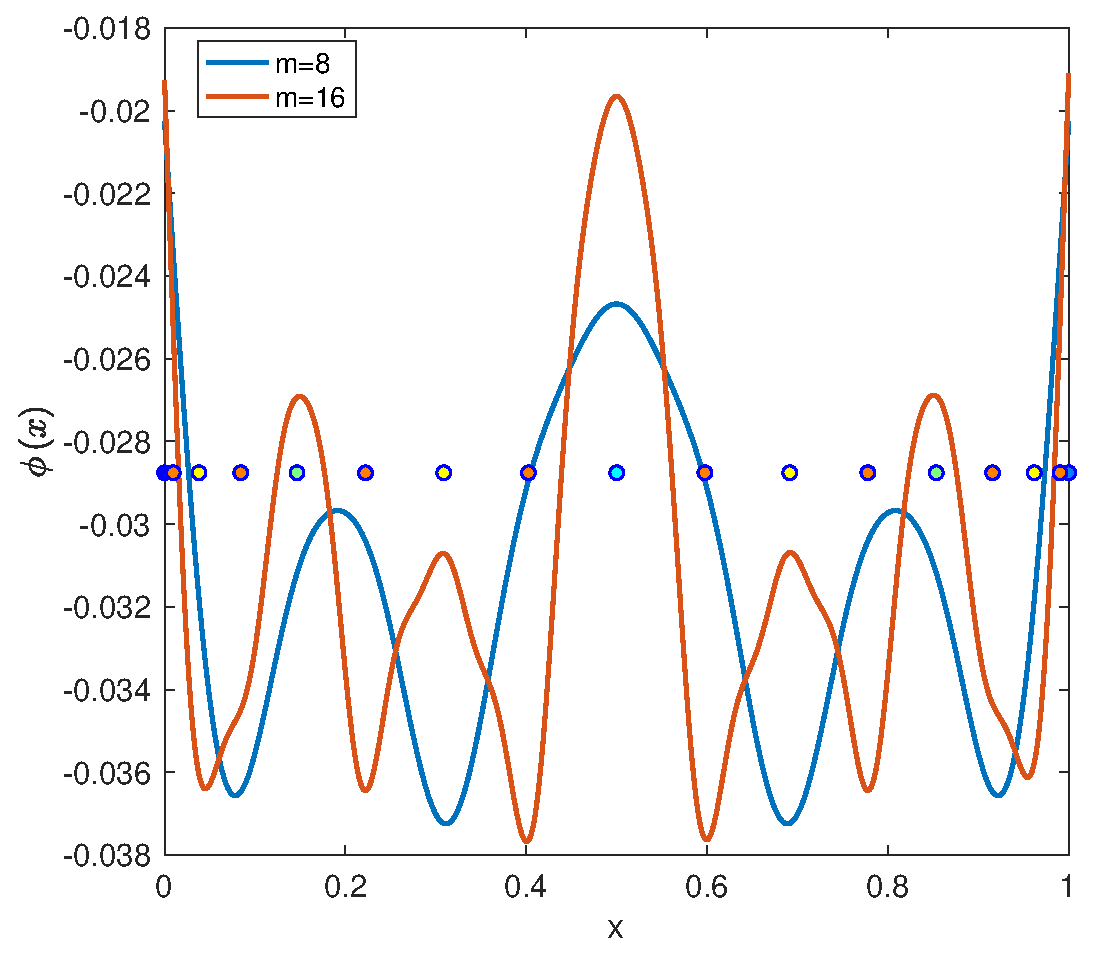
\includegraphics[width=2.2in]{images/06b-Logistic_findeigen_m8m16.eps}}
				\centerline{logistic map}
			\end{minipage}
		\end{figure}
	\end{frame}
	\begin{frame}{多峰映射}
		\begin{figure}
			\begin{minipage}{0.45\linewidth}
				\centerline{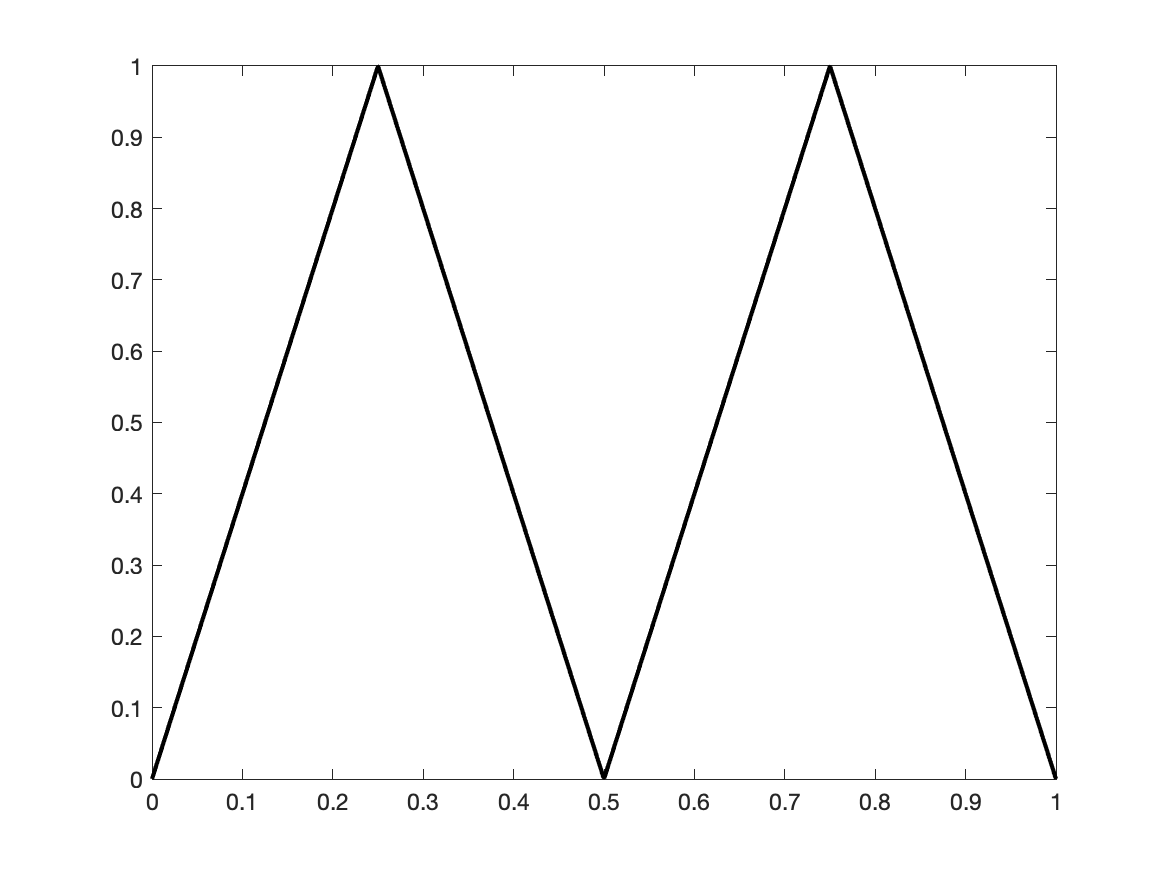
\includegraphics[width=2.2in]{images/Tents5_phase_d0.png}}
				\centerline{双峰映射}
			\end{minipage}
			\hfill
			\begin{minipage}{0.45\linewidth}
				\centerline{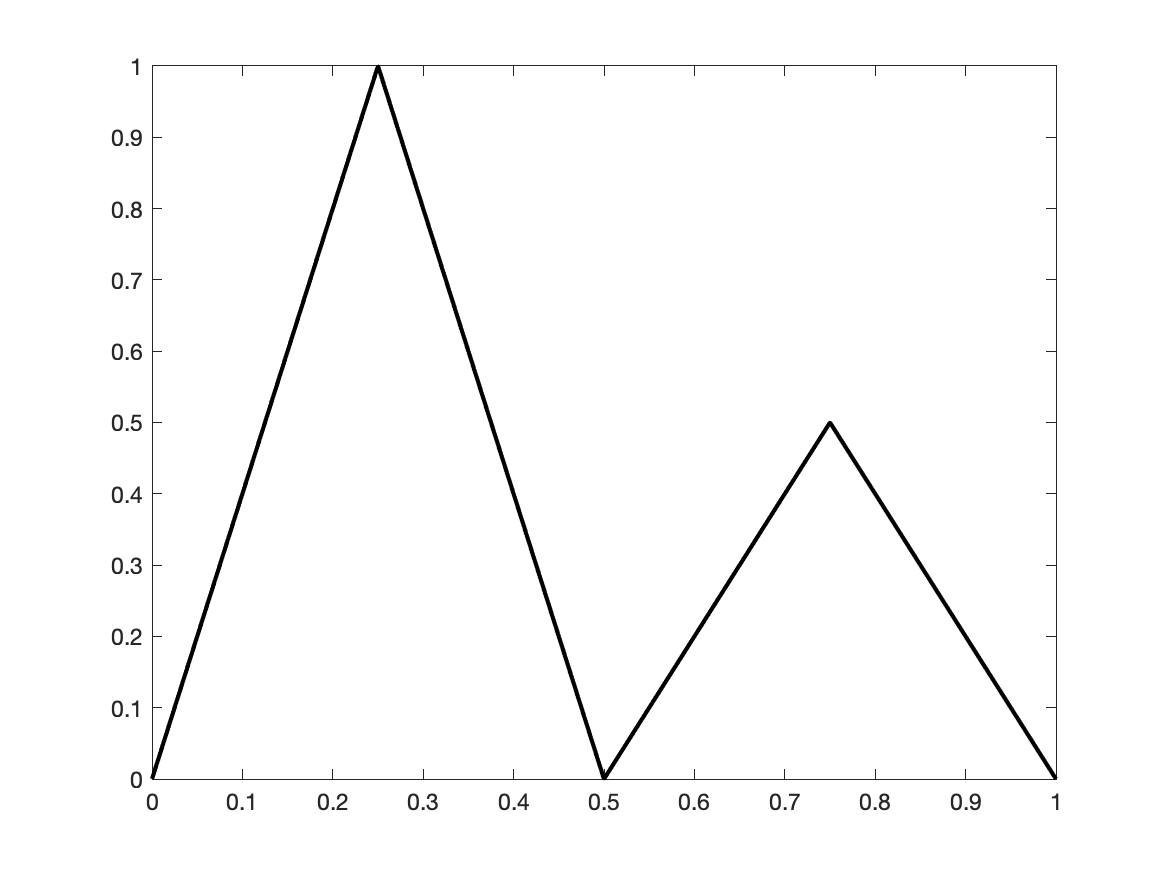
\includegraphics[width=2.2in]{images/Tents5l_phase_d0.png}}
				\centerline{大小峰映射}
			\end{minipage}
		\end{figure}
    \end{frame}
	\begin{frame}{多峰映射的本征函数(最大)}
		\begin{figure}
			\begin{minipage}{0.45\linewidth}
				\centerline{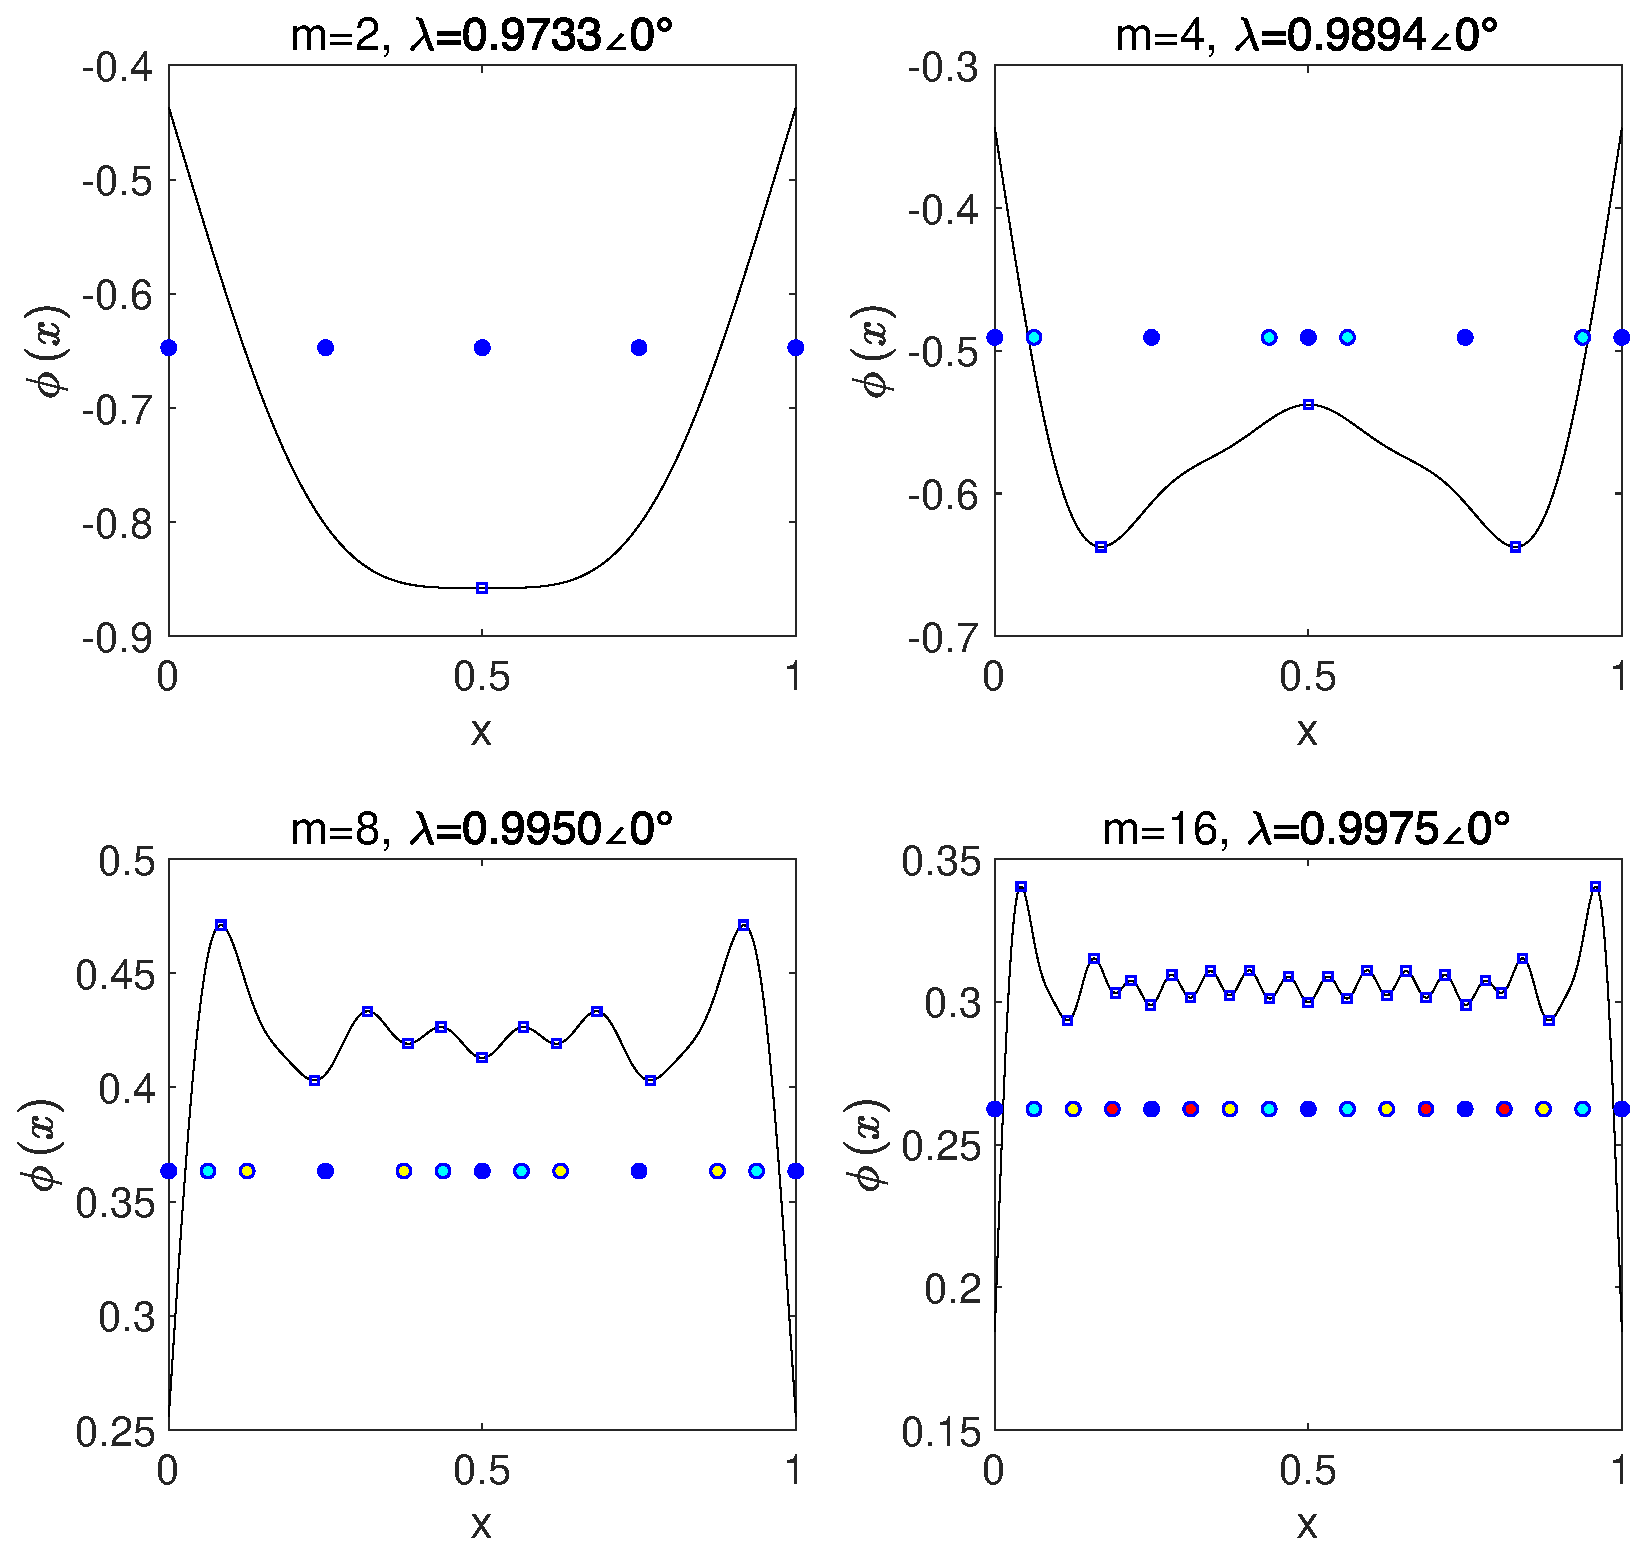
\includegraphics[width=2.2in]{images/07a-Tents51_eigen_Gauss_n1000_m2-4-8-16_d0.eps}}
				\centerline{双峰映射}
			\end{minipage}
			\hfill
			\begin{minipage}{0.45\linewidth}
				\centerline{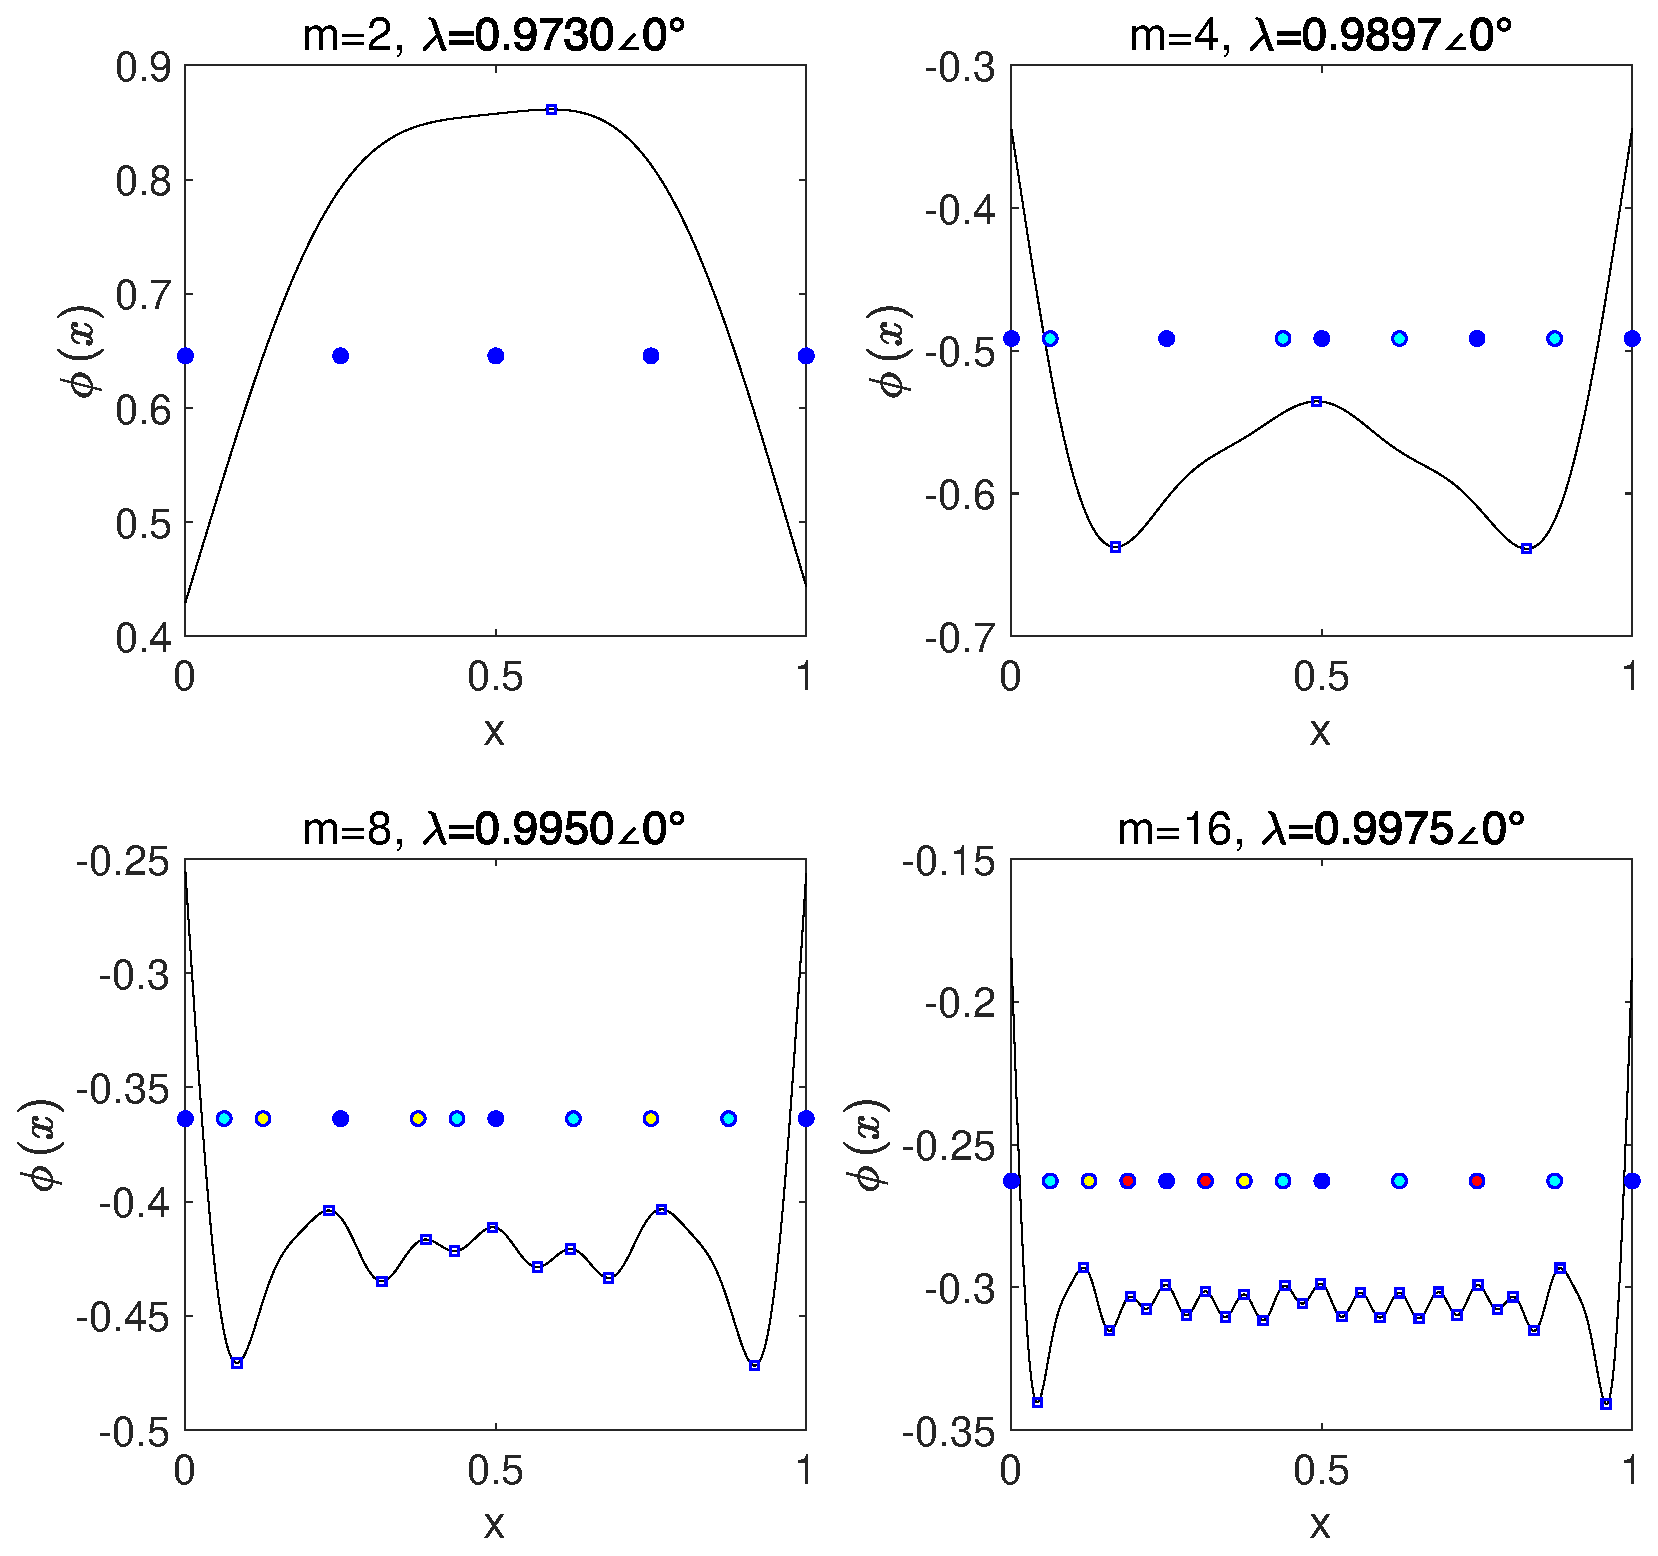
\includegraphics[width=2.2in]{images/07b-Tents5l1_eigen_Gauss_n1000_m2-4-8-16_d0.eps}}
				\centerline{大小峰映射}
			\end{minipage}
		\end{figure}
	\end{frame}
	\begin{frame}{多峰映射的本征函数(次大)}
		\begin{figure}
			\begin{minipage}{0.45\linewidth}
				\centerline{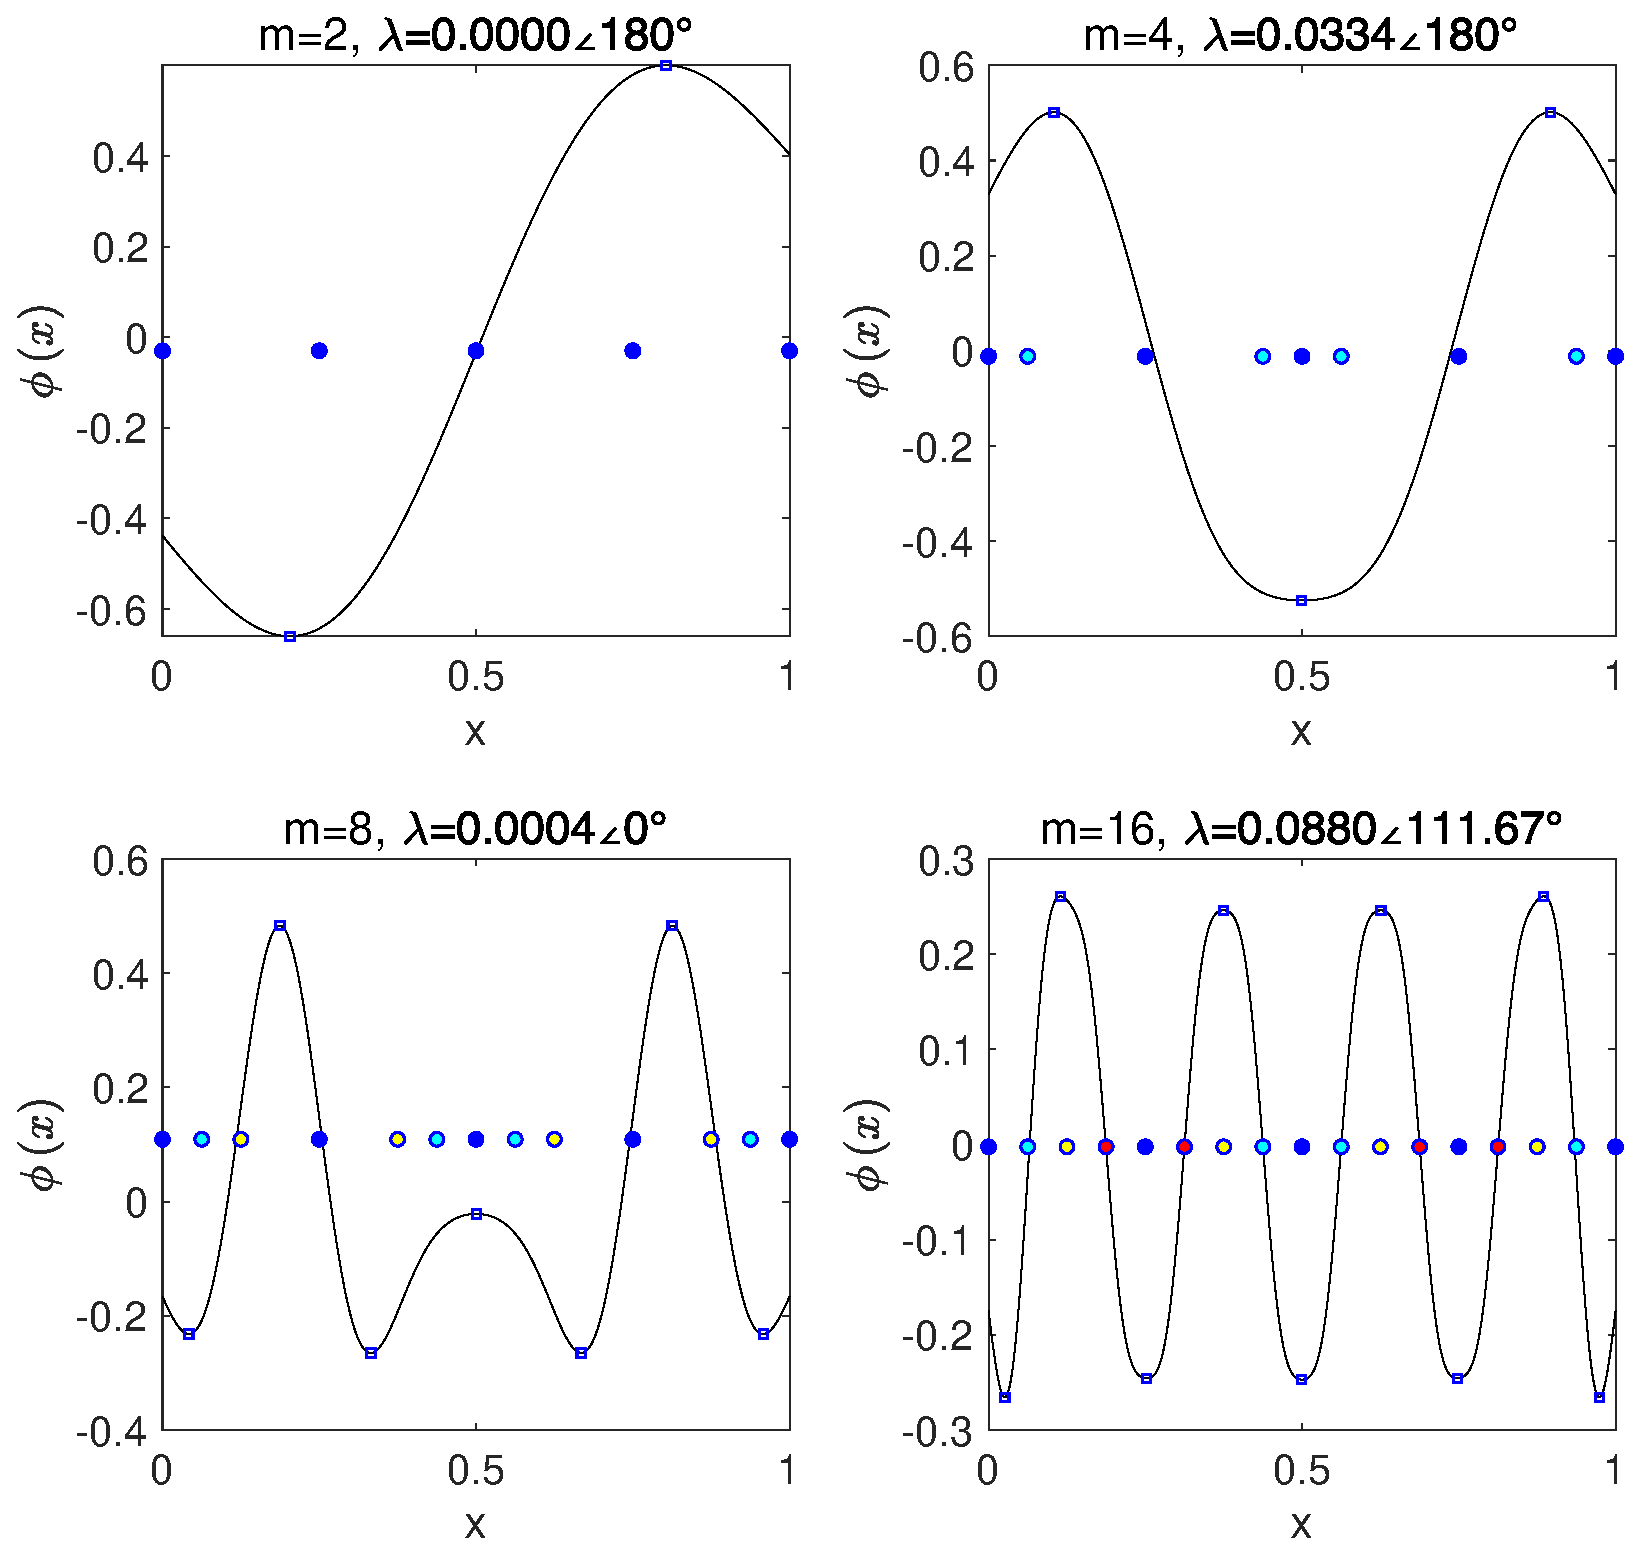
\includegraphics[width=2.2in]{images/08a-Tents52_eigen_Gauss_n1000_m2-4-8-16_d0.eps}}
				\centerline{双峰映射}
			\end{minipage}
			\hfill
			\begin{minipage}{0.45\linewidth}
				\centerline{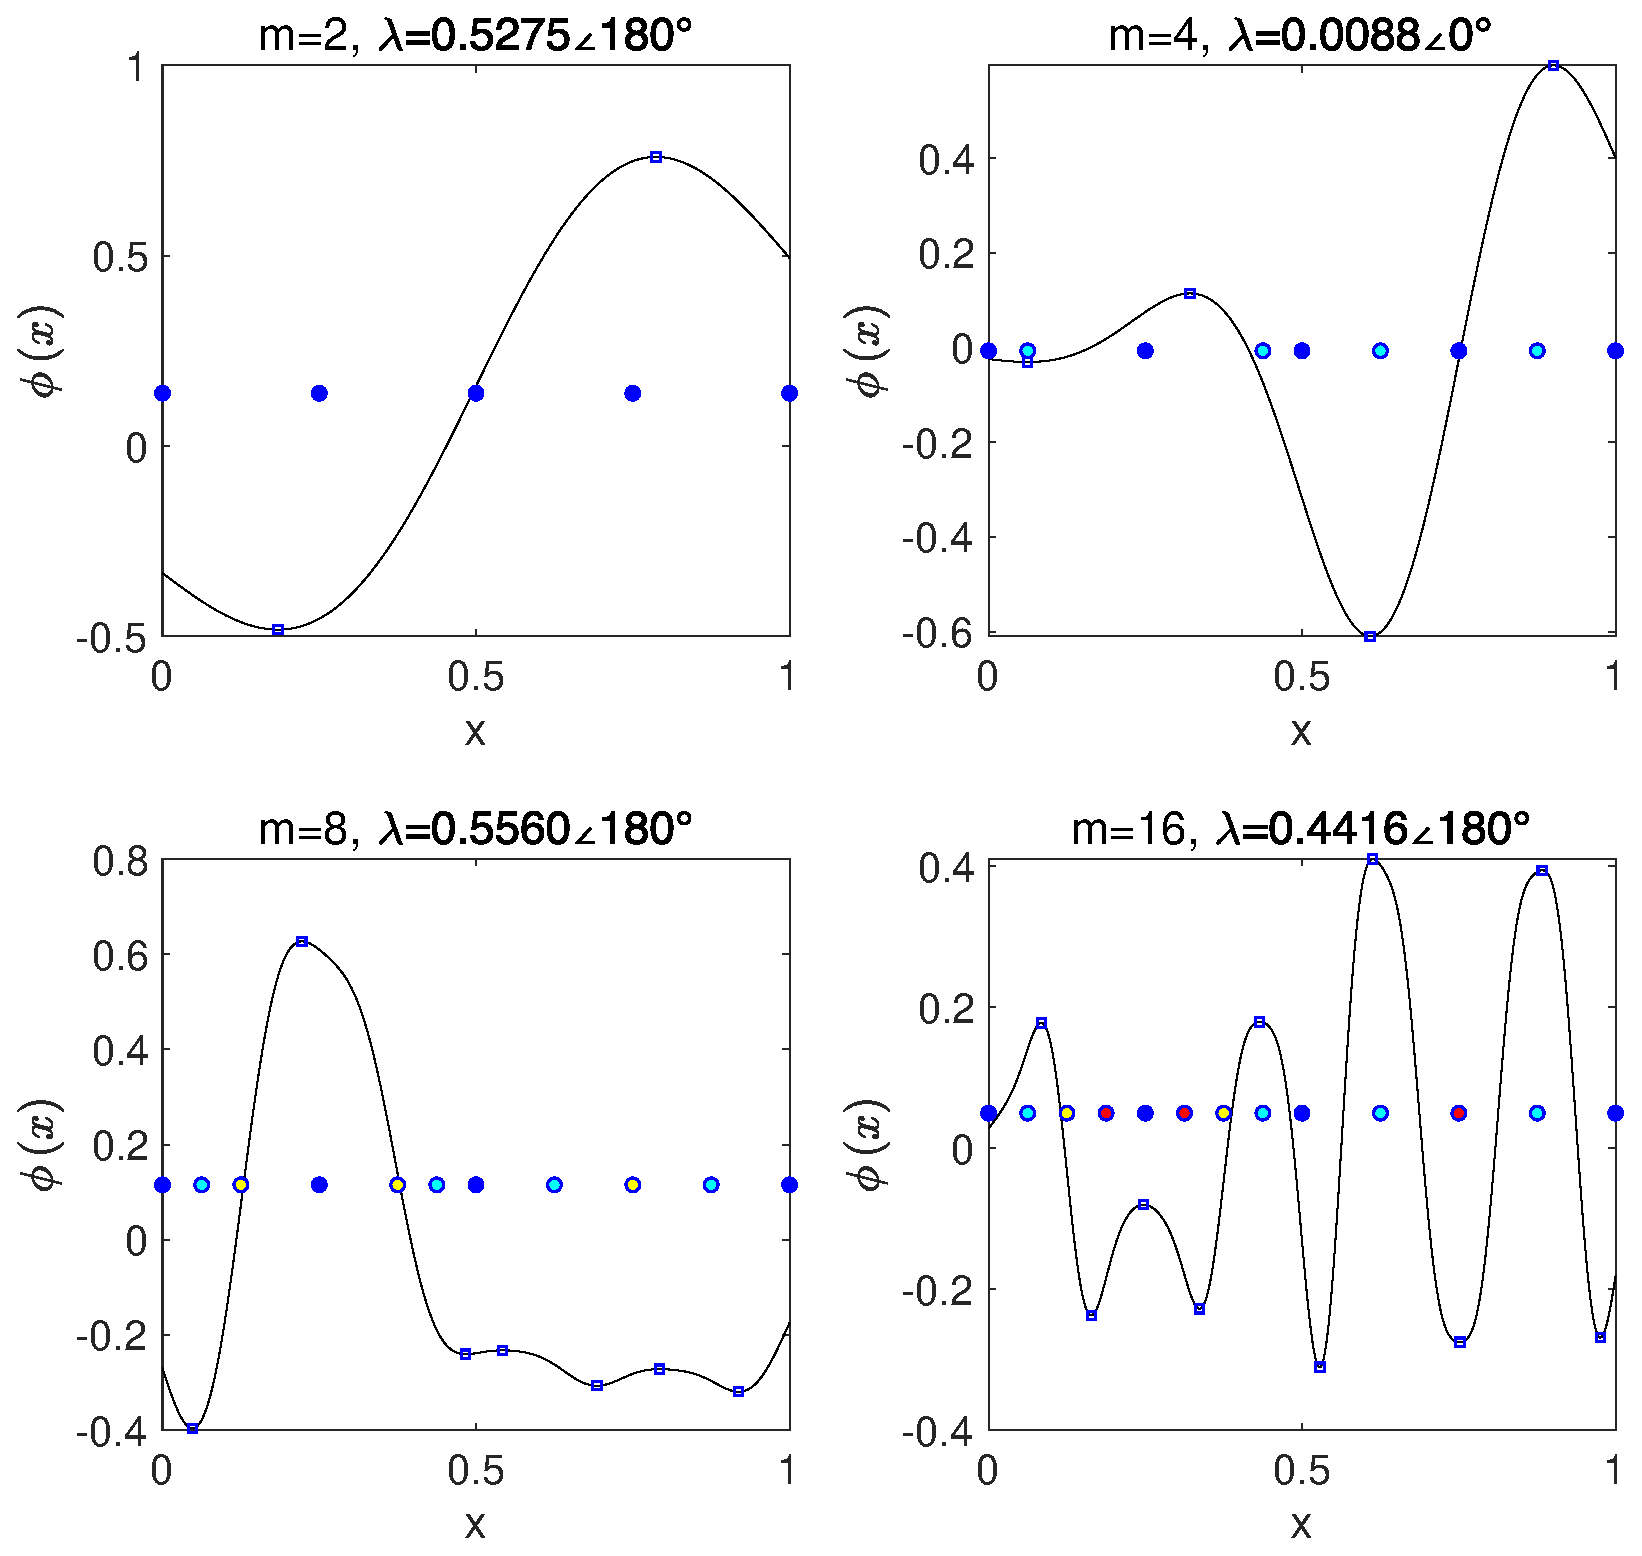
\includegraphics[width=2.2in]{images/08b-Tents5l2_eigen_Gauss_n1000_m2-4-8-16_d0.eps}}
				\centerline{大小峰映射}
			\end{minipage}
		\end{figure}
	\end{frame}
	
	\subsubsection{二维映射:Henon Map}
		\begin{frame}{Henon Map}
		\begin{block}{动力学方程}
			\centering
			\begin{math}
			\begin{cases}
				x_{n+1}=y_n+1-ax_n^2\\
				y_{n+1}=bx_n
			\end{cases}\ x,y\in [-1.5,1.5]
			\end{math}
		\end{block}
		我们选取a=1.4,b=0.3使其处于混沌状态。\\
		两个不动点:(0.6314,0.1894)
和(-1.1314,-0.3394)
		\begin{figure}
			\begin{minipage}{0.4\linewidth}
				\centering
				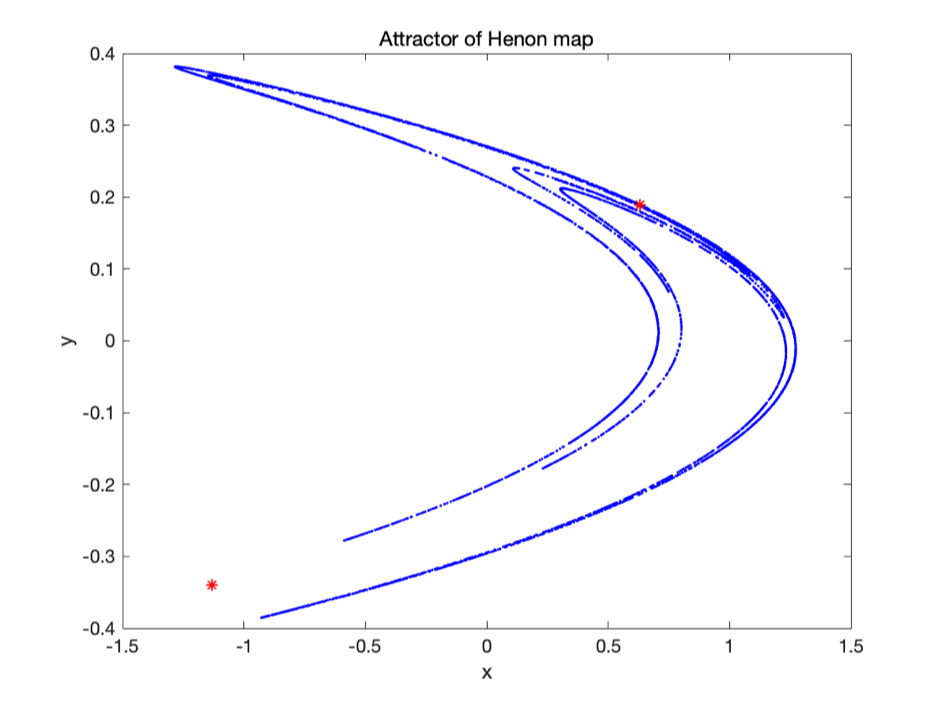
\includegraphics[width=1.8in]{figure/henon_phase}
				\caption{Henon map相图}
			\end{minipage}
		\end{figure}
		\end{frame}
	\begin{frame}{Henon Map-二维高级基函数下的本征函数}
		\centerline{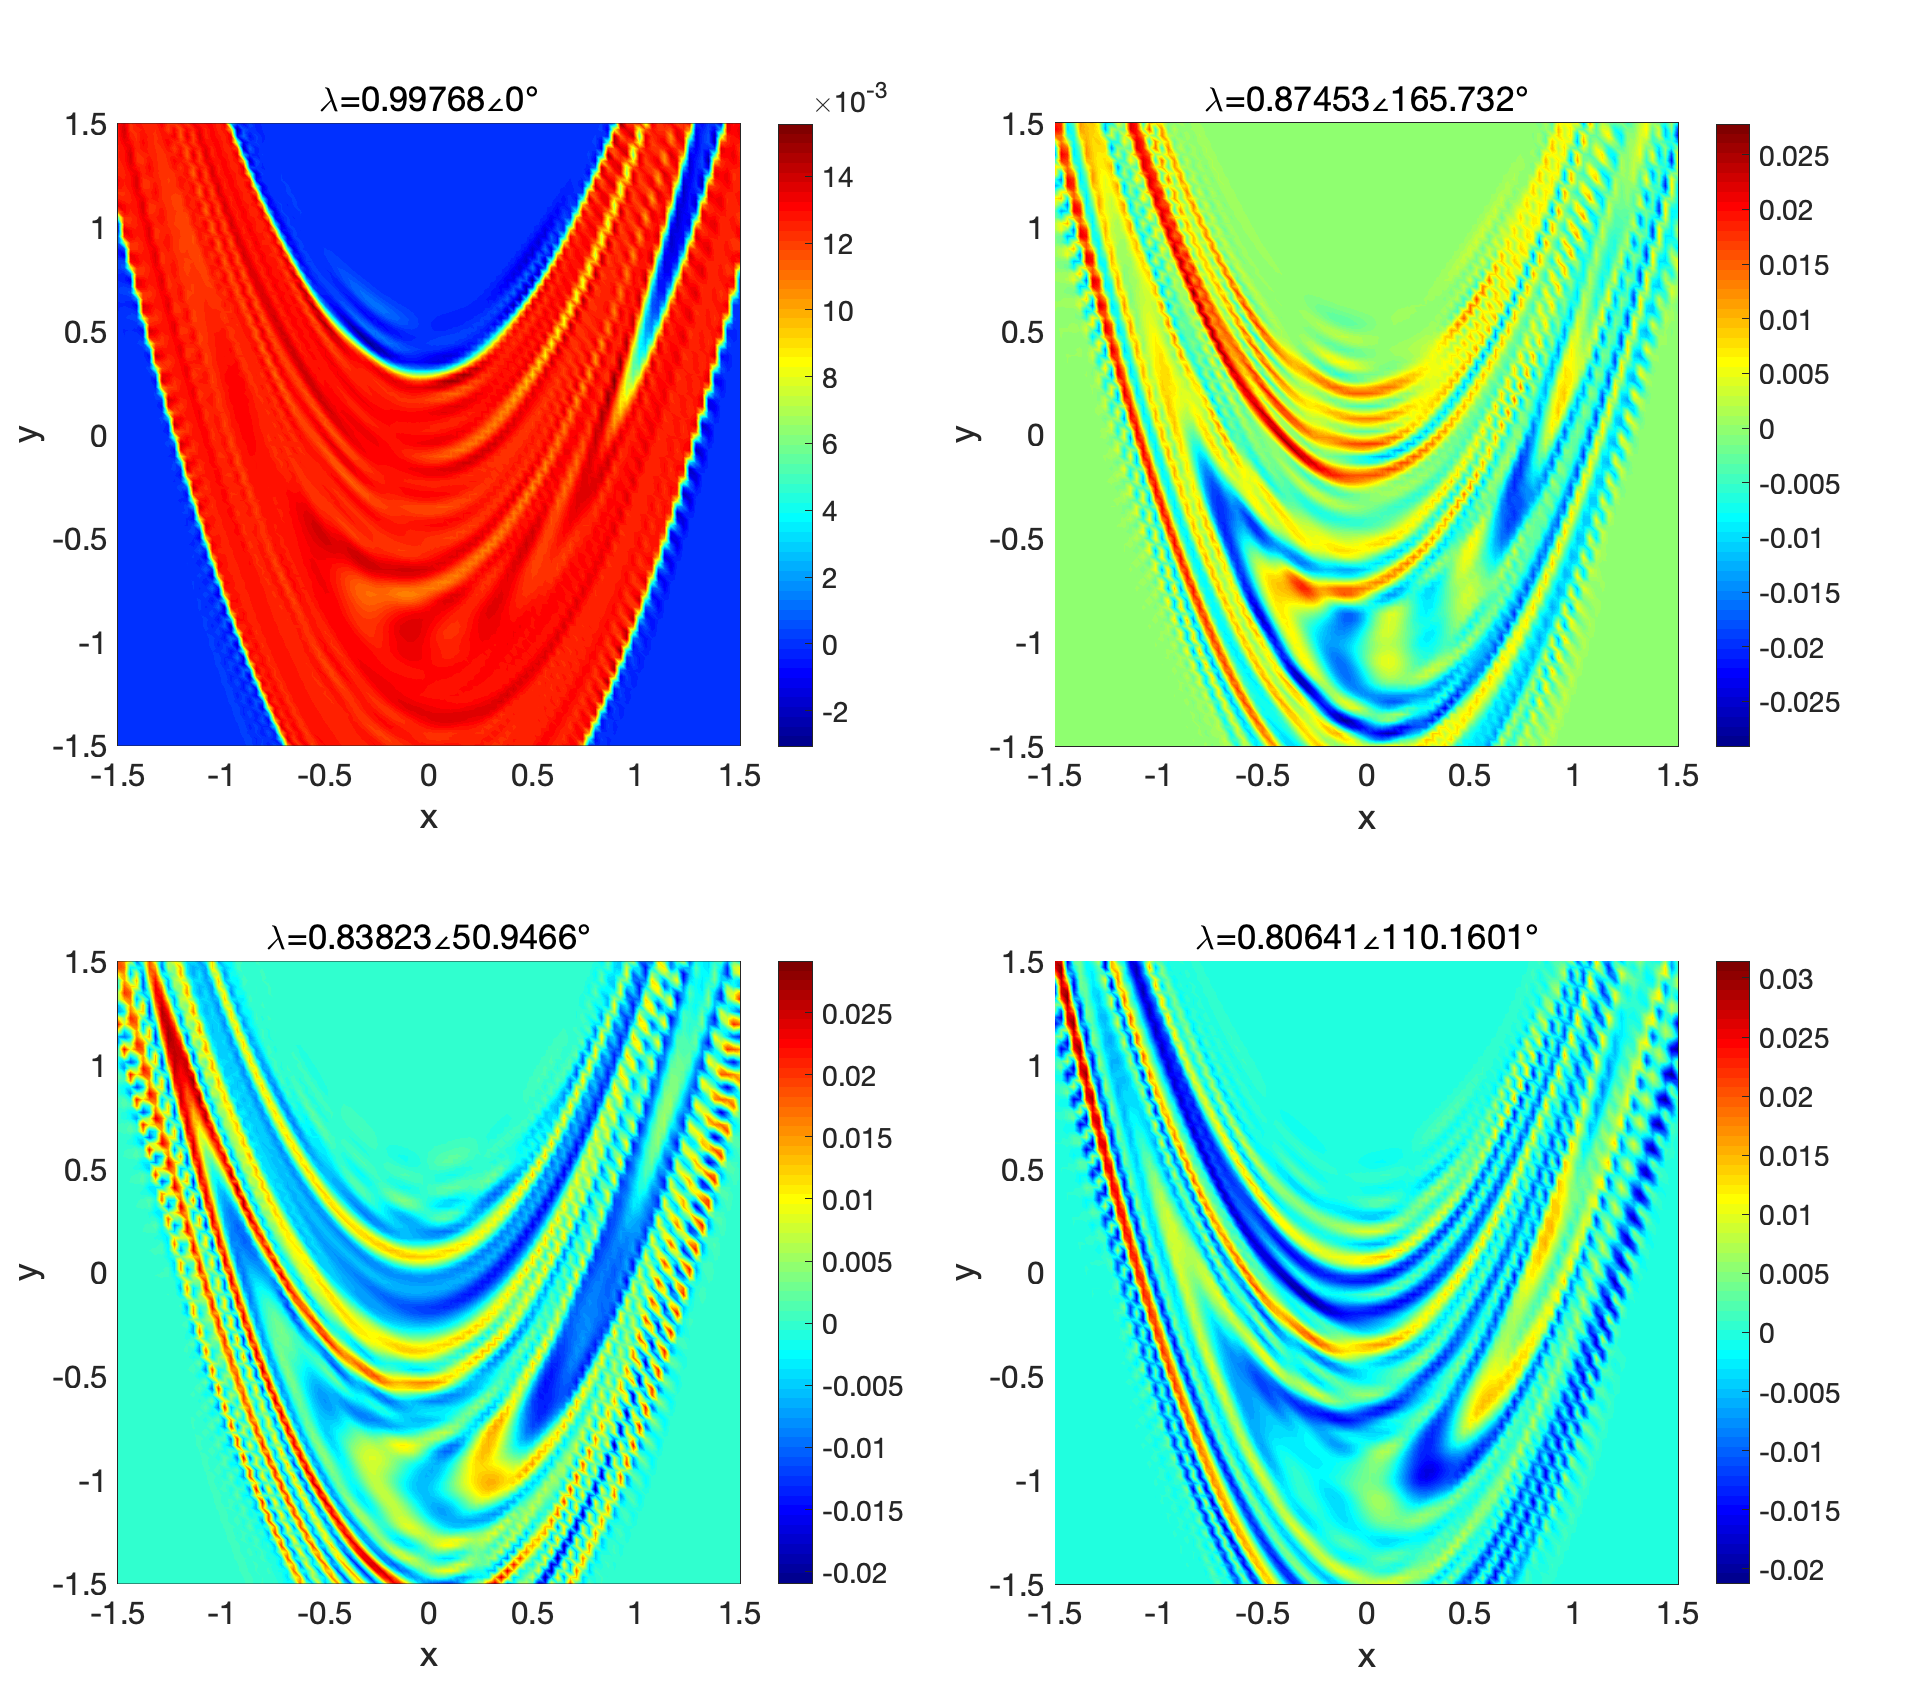
\includegraphics[width=3.5in]{images/09-Henon_eigen_Gauss_n100m50md45.eps}}
	\end{frame}
    \begin{frame}{Henon Map-周期轨道与线性化}
    	\centerline{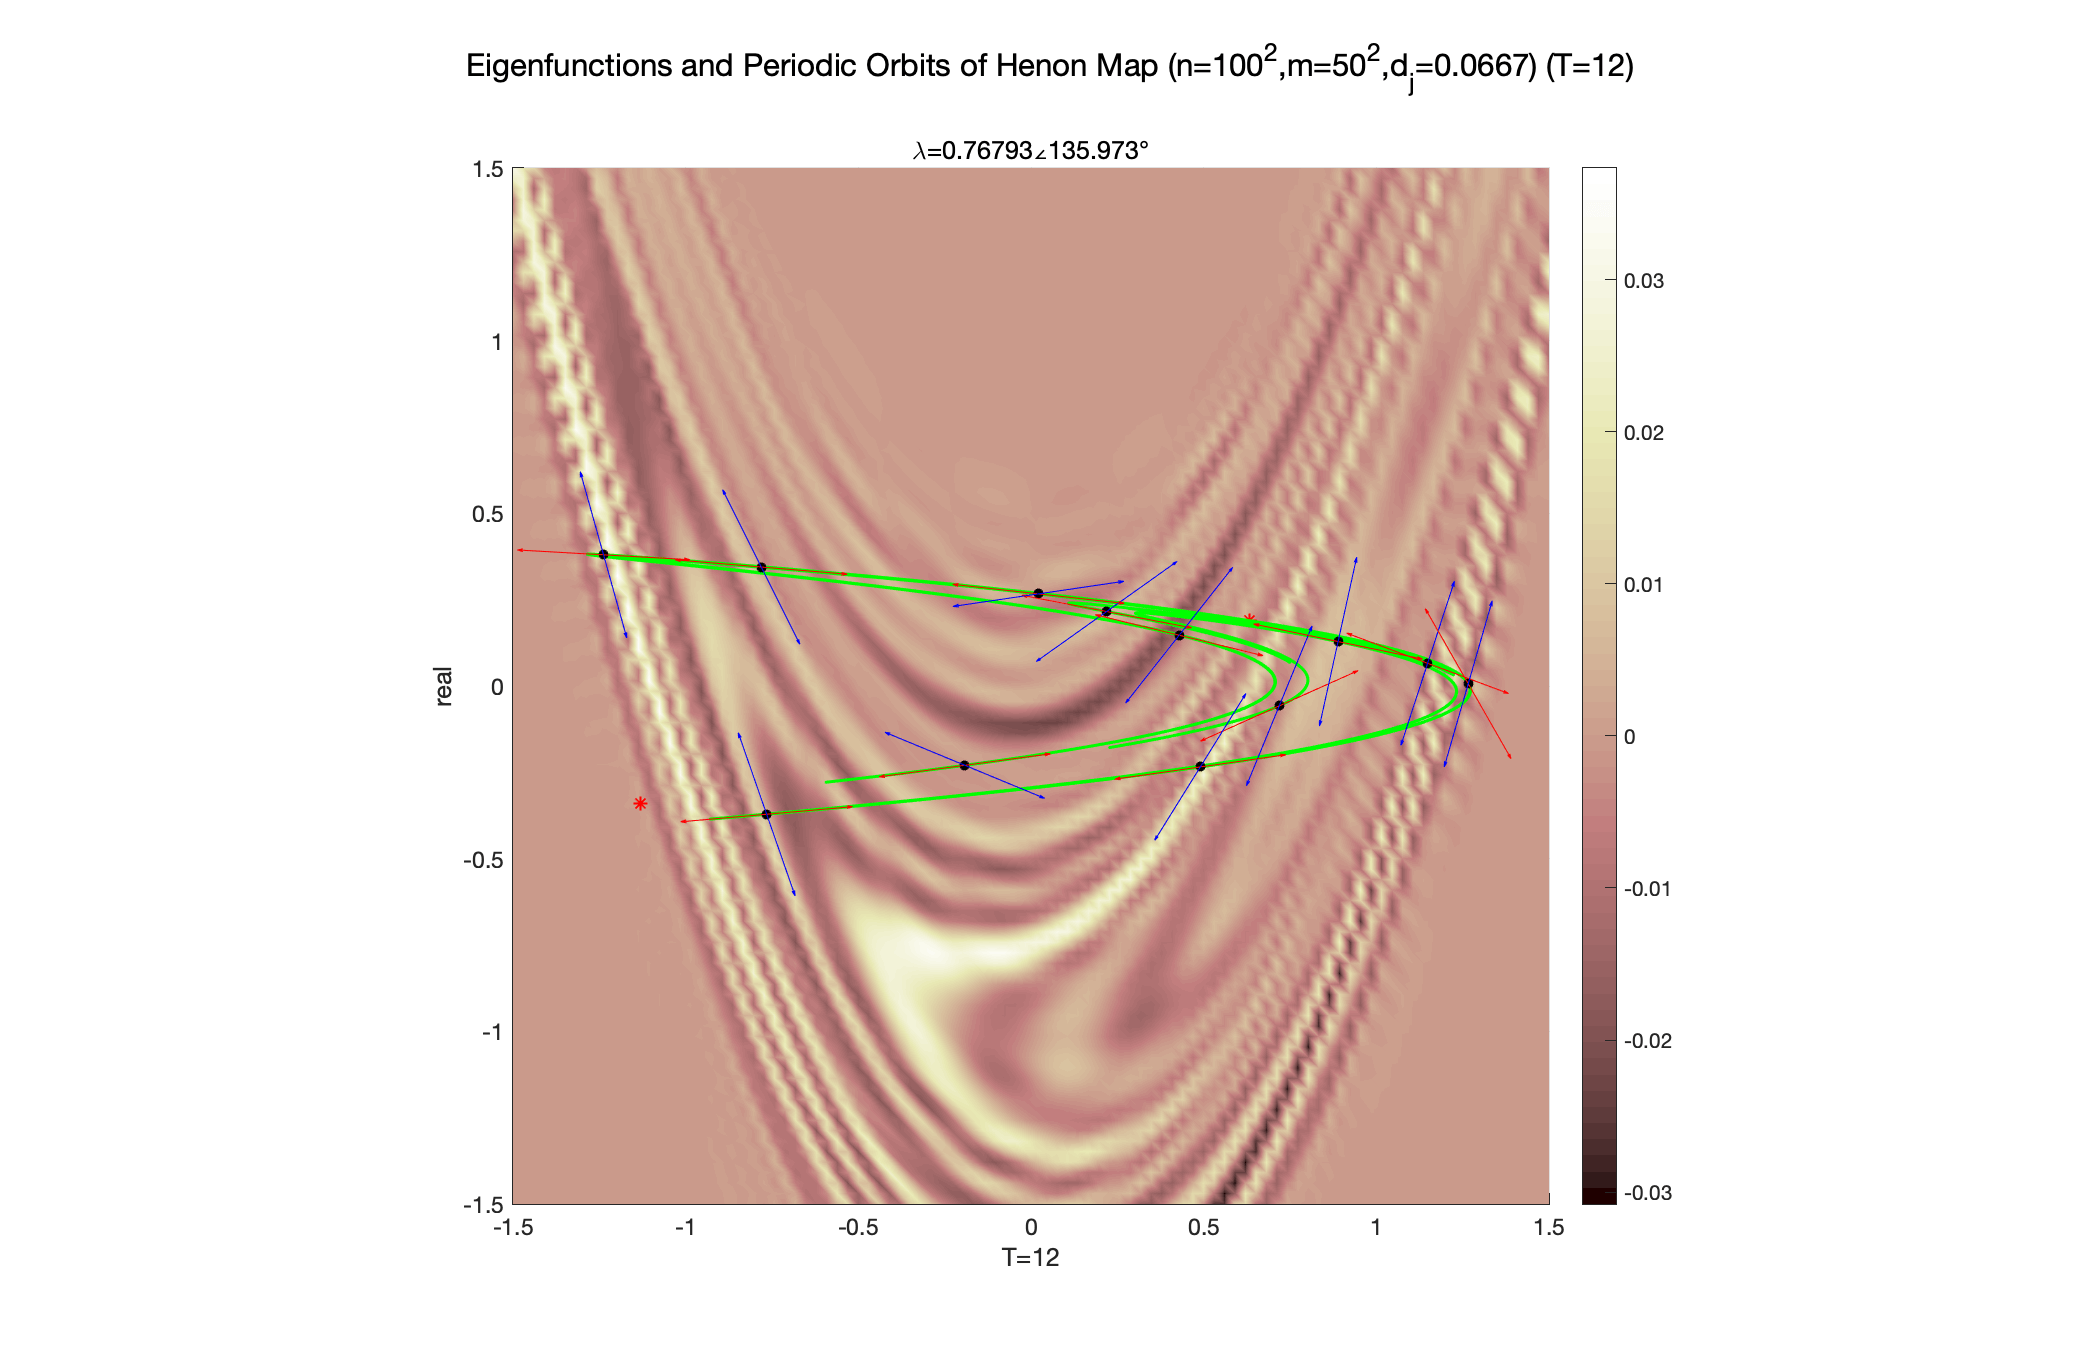
\includegraphics[width=4.5in]{images/Henon_eigen_Gauss_period1_n100m50T12.png}}
    \end{frame}
	 \begin{frame}{Henon Map-周期轨道与不稳定流型}
		\centerline{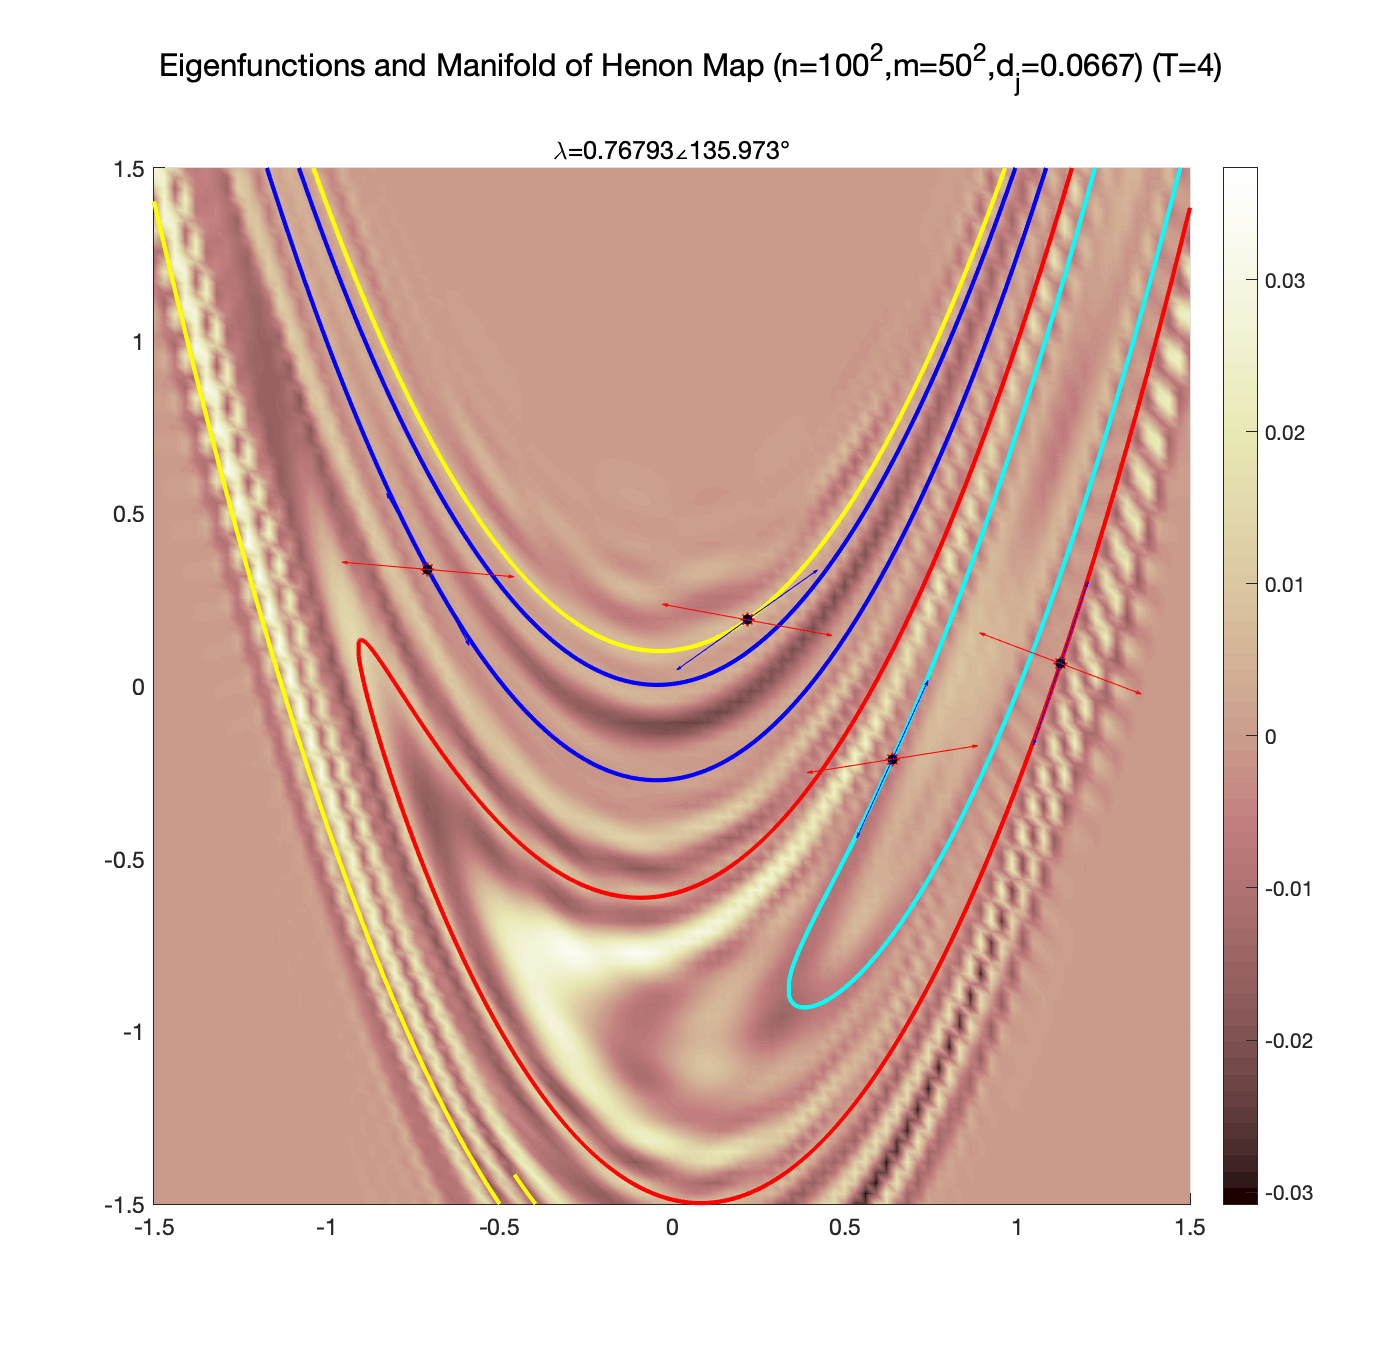
\includegraphics[width=3.2in]{images/Henon_eigen_Gauss_manifold_n100m50T4.png}}
	\end{frame}
	\begin{frame}{Henon Map的像点和原像点(边界点)}
		\begin{figure}
			\begin{minipage}{0.45\linewidth}
				\centerline{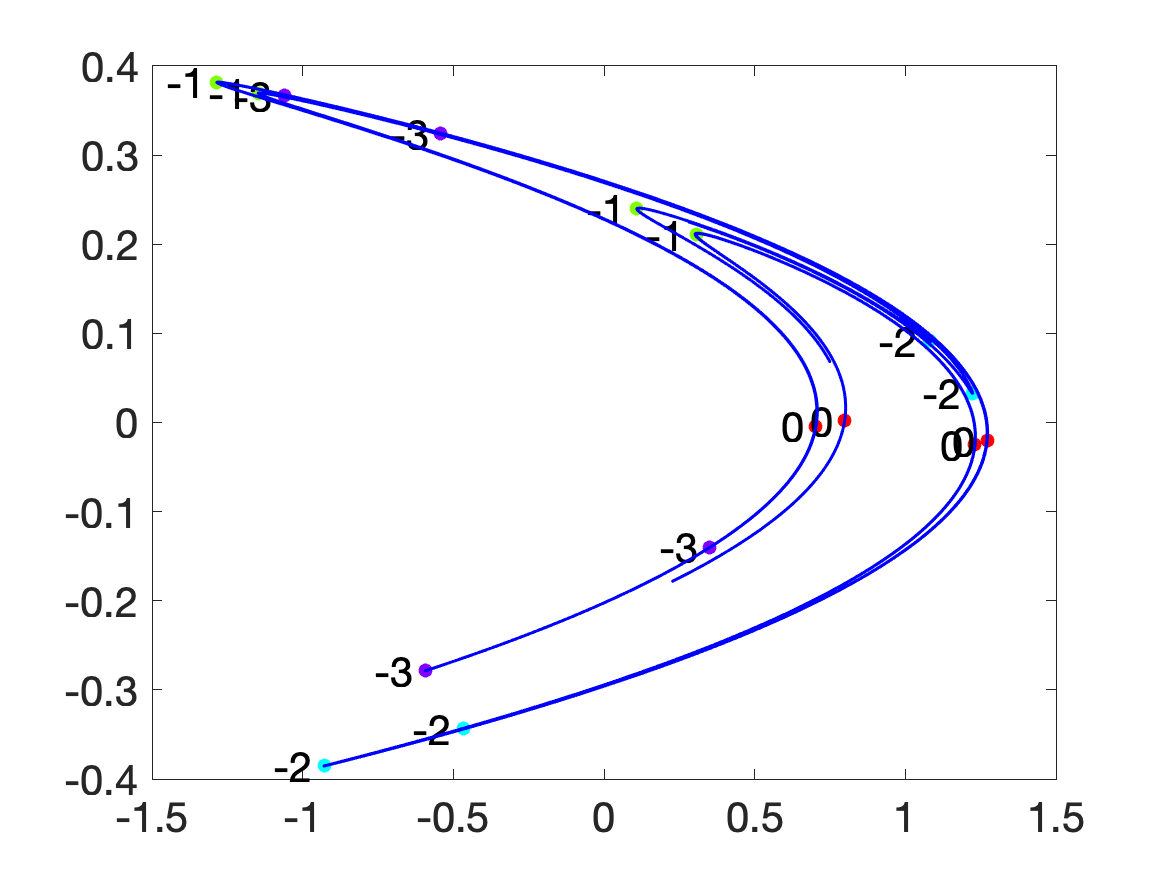
\includegraphics[width=2.4in]{images/Henon_boundary_forward.png}}
				\centerline{正向迭代}
			\end{minipage}
			\hfill
			\begin{minipage}{0.45\linewidth}
				\centerline{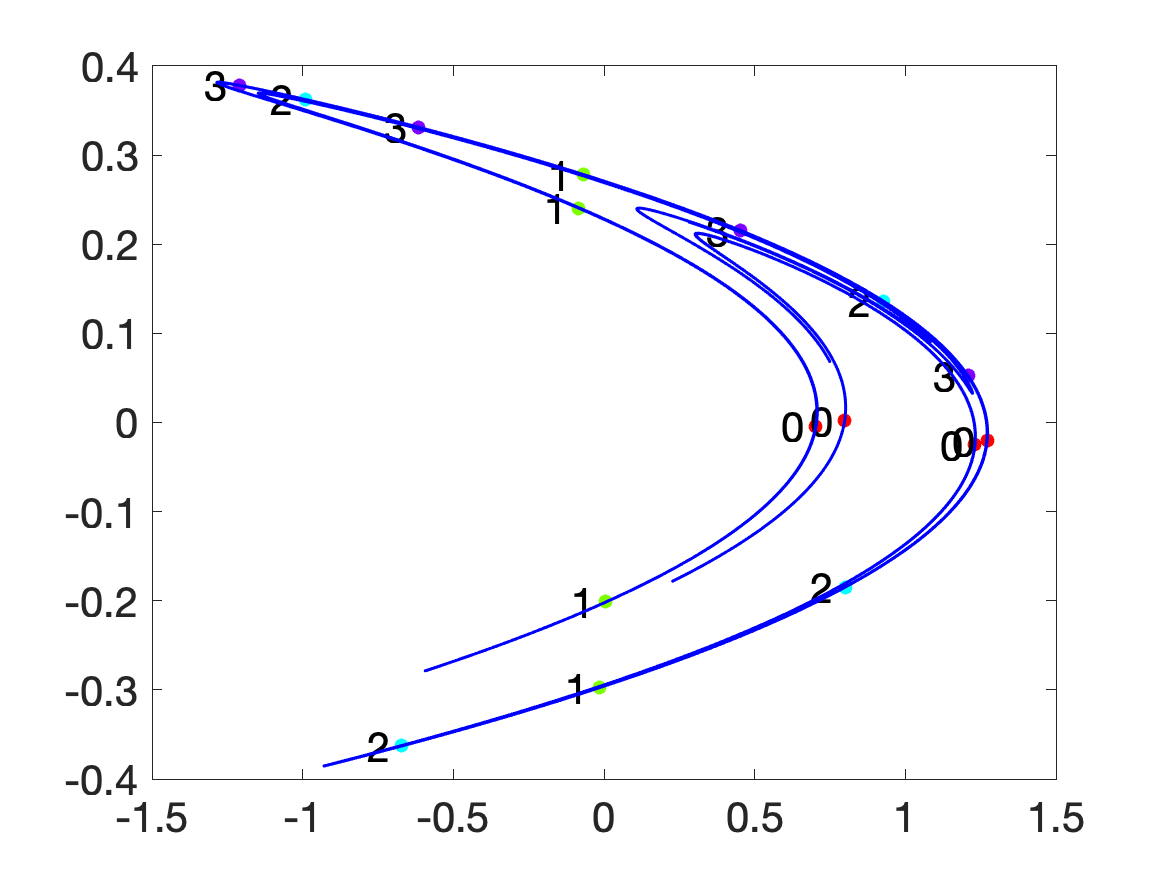
\includegraphics[width=2.4in]{images/Henon_boundary_reverse.png}}
				\centerline{反向迭代}
			\end{minipage}
		\end{figure}
	\end{frame}
	\begin{frame}{Henon Map-二维自然基函数下的本征函数}
		\centerline{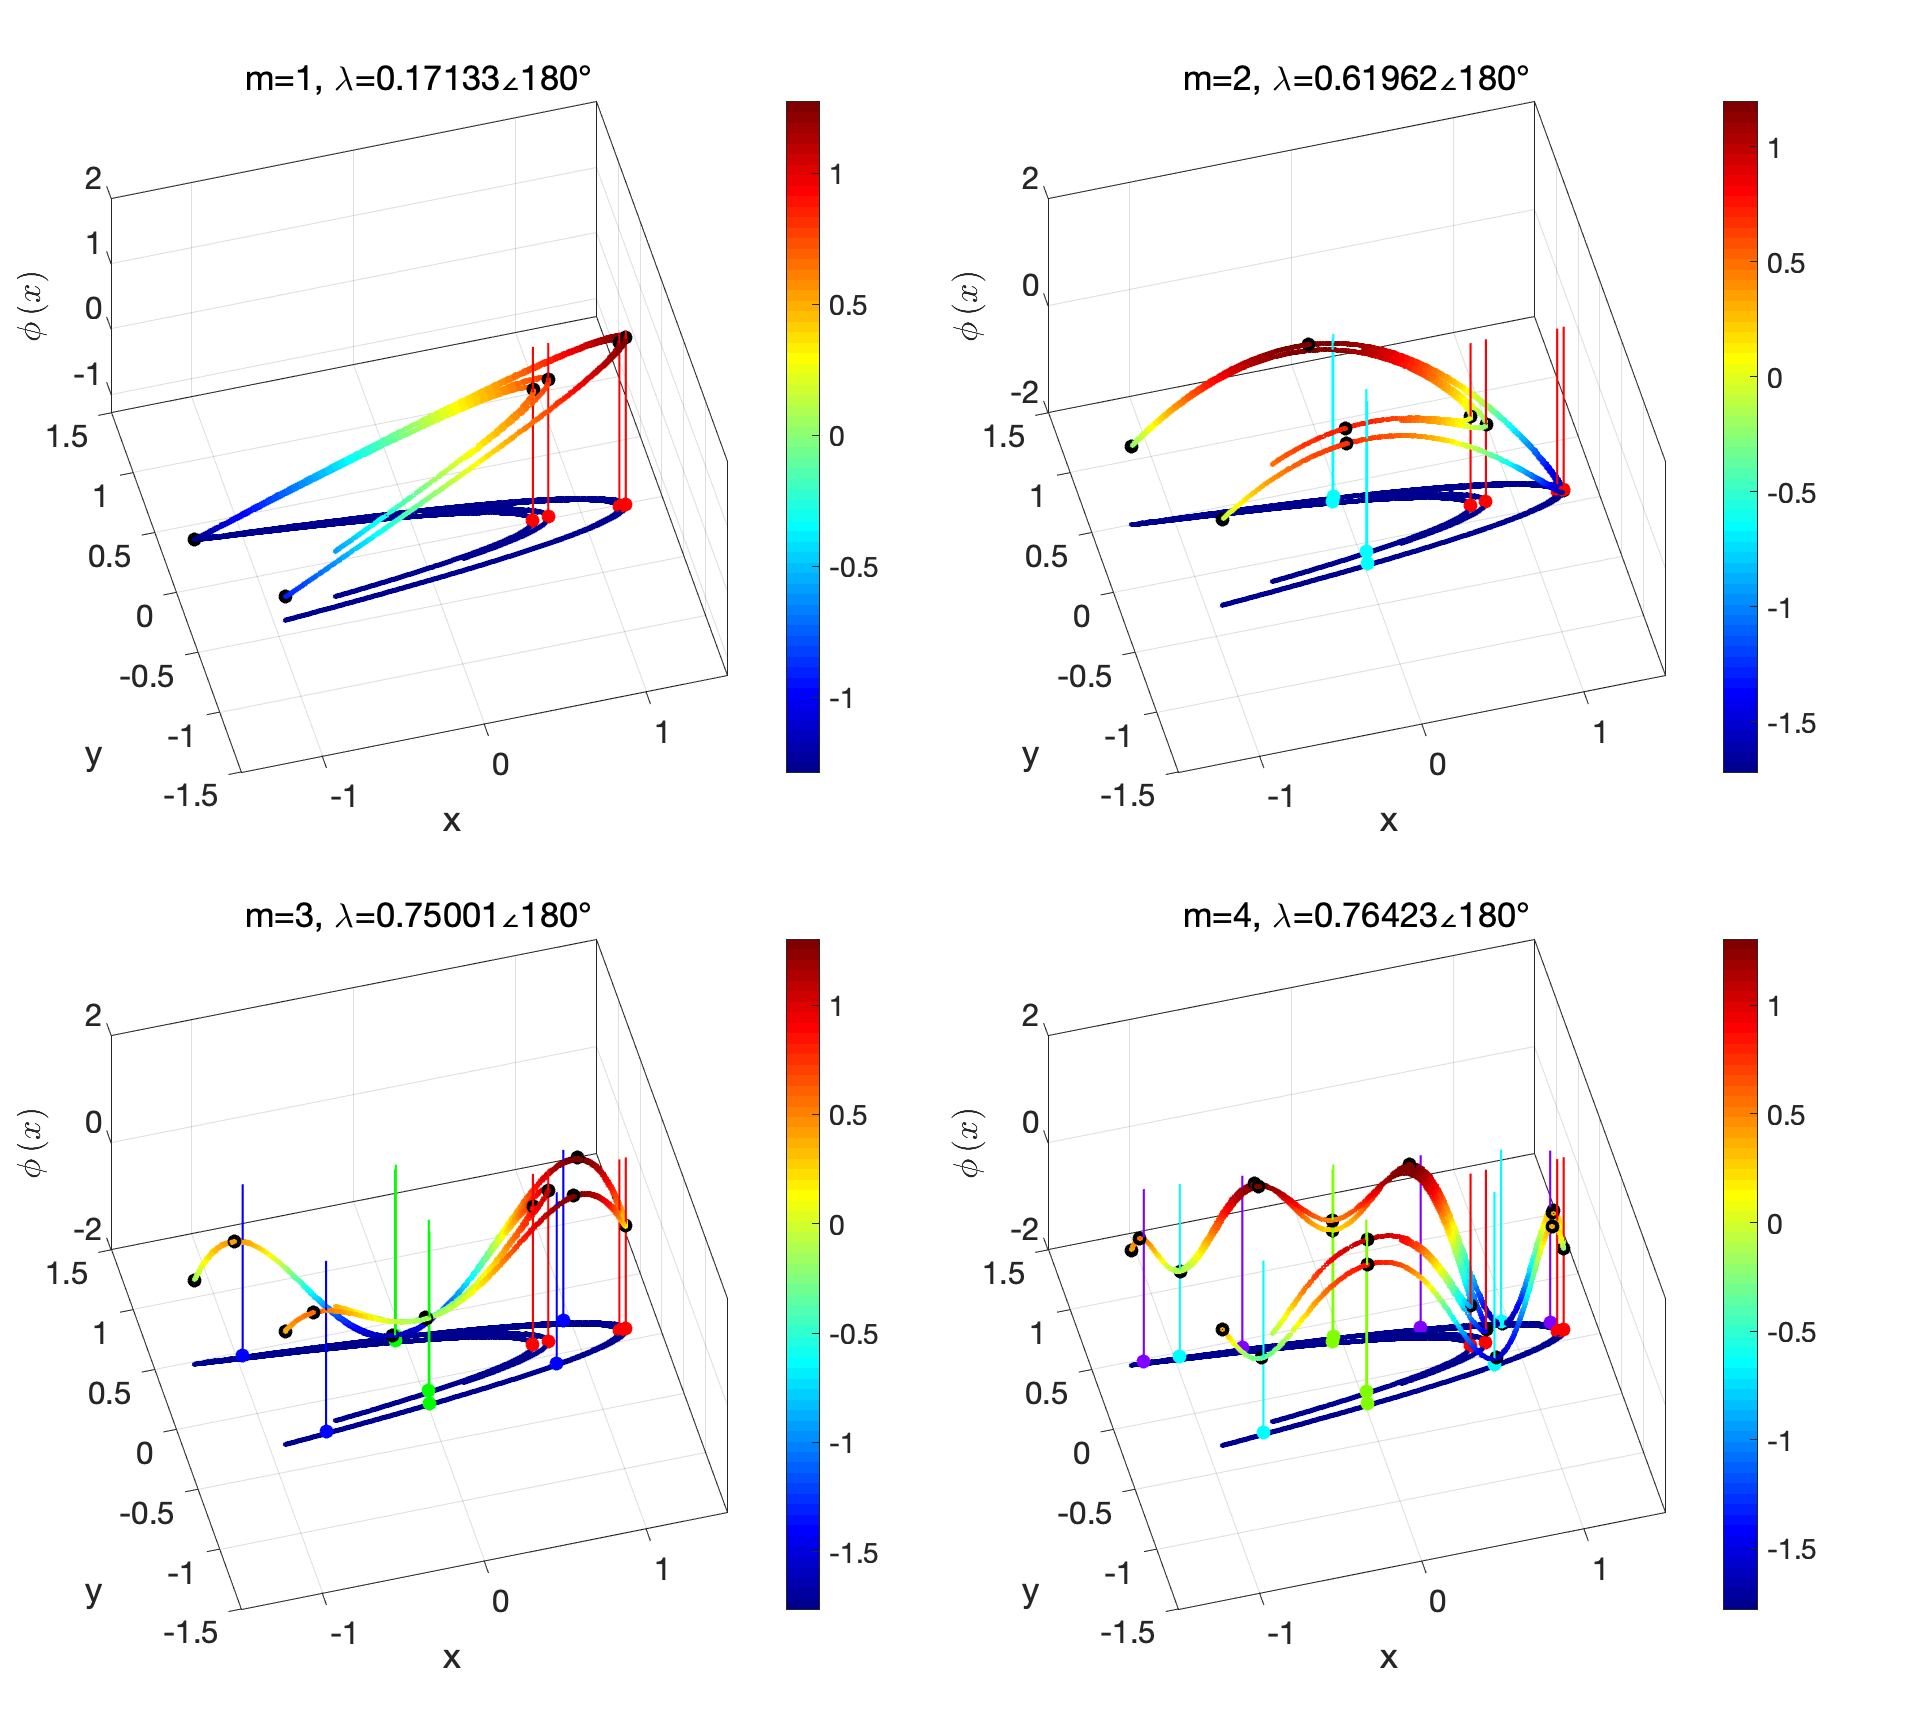
\includegraphics[width=3.5in]{images/11-Henon_eigen_natural_attr_n10000m1-2-3-4.eps}}
	\end{frame}
	\newcommand{\pos}[2]{(#1,#2)}
	\begin{frame}
		\tiny \centering
		\begin{tabular}{cccc}
			\textrm{$m$}&\textrm{$l$}&\textrm{极值点}&\textrm{边界点}\\
			\hline
			\multirow{4}{*}{$1$}& \multirow{4}{*}{$0$} & \pos{\ 0.7079}{\ 0.0120} & \pos{\ 0.7021}{-0.0044} \\
			& & \pos{\ 0.8019}{\ 0.0191} & \pos{\ 0.7986}{\ 0.0019} \\
			& & \pos{\ 1.2326}{-0.0153} & \pos{\ 1.2307}{-0.0249} \\
			& & \pos{\ 1.2729}{-0.0091} & \pos{\ 1.2717}{-0.0205} \\
			\hline
			\multirow{8}{*}{$2$}& \multirow{4}{*}{$0$} & \pos{\ 0.7052}{-0.0009} & \pos{\ 0.7021}{-0.0044} \\
			& & \pos{\ 0.7995}{\ 0.0041} & \pos{\ 0.7986}{\ 0.0019} \\
			& & \pos{\ 1.2720}{-0.0192} & \pos{\ 1.2307}{-0.0249} \\
			& & \pos{\ 1.2720}{-0.0192} & \pos{\ 1.2717}{-0.0205} \\ \cline{2-4}
			& \multirow{4}{*}{$1$} & \pos{-0.1418}{-0.3100} & \pos{-0.0148}{-0.2976} \\
			& & \pos{-0.1258}{-0.2206} & \pos{\ 0.0065}{-0.2013} \\
			& & \pos{-0.2164}{\ 0.2936} & \pos{-0.0832}{\ 0.2403} \\
			& & \pos{-0.2164}{\ 0.2936} & \pos{-0.0682}{\ 0.2782} \\
			\hline
			\multirow{12}{*}{$3$}& \multirow{4}{*}{$0$} & \pos{\ 0.7045}{-0.0026} & \pos{\ 0.7021}{-0.0044} \\
			& & \pos{\ 0.7995}{\ 0.0041} & \pos{\ 0.7986}{\ 0.0019} \\
			& & \pos{\ 1.2713}{-0.0217} & \pos{\ 1.2307}{-0.0249} \\
			& & \pos{\ 1.2713}{-0.0217} & \pos{\ 1.2717}{-0.0205} \\ \cline{2-4}
			& \multirow{4}{*}{$1$} & \pos{-0.0330}{-0.2981} & \pos{-0.0148}{-0.2976} \\
			& & \pos{-0.0121}{-0.2041} & \pos{\ 0.0065}{-0.2013} \\
			& & \pos{-0.0982}{\ 0.2431} & \pos{-0.0832}{\ 0.2403} \\
			& & \pos{-0.0862}{\ 0.2802} & \pos{-0.0682}{\ 0.2782} \\ \cline{2-4}
			& \multirow{4}{*}{$2$} & \pos{-1.0459}{\ 0.3549} & \pos{-0.9918}{\ 0.3625} \\
			& & \pos{-0.7503}{-0.3700} & \pos{-0.6711}{-0.3630} \\
			& & \pos{\ 0.9130}{-0.1574} & \pos{\ 0.8011}{-0.1846} \\
			& & \pos{\ 1.0081}{\ 0.1176} & \pos{\ 0.9275}{\ 0.1361} \\
			\hline
			\multirow{16}{*}{$4$}& \multirow{4}{*}{$0$} & \pos{\ 0.7045}{-0.0026} & \pos{\ 0.7021}{-0.0044} \\
			& & \pos{\ 0.8002}{\ 0.0059} & \pos{\ 0.7986}{\ 0.0019} \\
			& & \pos{\ 1.2713}{-0.0217} & \pos{\ 1.2307}{-0.0249} \\
			& & \pos{\ 1.2713}{-0.0217} & \pos{\ 1.2717}{-0.0205} \\ \cline{2-4}
			& \multirow{4}{*}{$1$} & \pos{-0.0086}{-0.2954} & \pos{-0.0148}{-0.2976} \\
			& & \pos{\ 0.0138}{-0.2002} & \pos{\ 0.0065}{-0.2013} \\
			& & \pos{-0.0856}{\ 0.2413} & \pos{-0.0832}{\ 0.2403} \\
			& & \pos{-0.0724}{\ 0.2787} & \pos{-0.0682}{\ 0.2782} \\ \cline{2-4}
			& \multirow{4}{*}{$2$} & \pos{-0.9937}{\ 0.3495} & \pos{-0.9918}{\ 0.3625} \\
			& & \pos{-0.6805}{-0.3638} & \pos{-0.6711}{-0.3630} \\
			& & \pos{\ 0.8132}{-0.1780} & \pos{\ 0.8011}{-0.1846} \\
			& & \pos{\ 0.9338}{\ 0.1347} & \pos{\ 0.9275}{\ 0.1361} \\ \cline{2-4}
			& \multirow{4}{*}{$3$} & \pos{\ 1.2205}{\ 0.0336} & \pos{\ 1.2084}{\ 0.0523} \\
			& & \pos{-1.2334}{\ 0.3797} & \pos{-1.2099}{\ 0.3783} \\
			& & \pos{-0.5413}{\ 0.3240} & \pos{-0.6154}{\ 0.3313} \\
			& & \pos{\ 0.3897}{\ 0.2237} & \pos{\ 0.4535}{\ 0.2154} \\
			\hline
		\end{tabular}
	\end{frame}

	\subsubsection{三维流:Lorenz System}
		\begin{frame}{Lorenz System}
		\begin{block}{动力学方程}
			\centering
			\begin{math}
			\begin{cases}
			\dot{x}=\sigma (y-x)\\
			\dot{y}=x(\gamma-z)-y\\
			\dot{z}=xy-\beta z
			\end{cases}\
			\end{math}
		\end{block}
		取$\beta=\frac{8}{3}$,$\rho=28$,$\sigma=10$使系统处于混沌状态,初始点(-1,3,4)\\
		三个不动点:(0,0,0)
、(-8.4853,8.4853,27)
、(8.4853,-8,4853,27)
		\begin{figure}
			\begin{minipage}{0.4\linewidth}
				\centering
				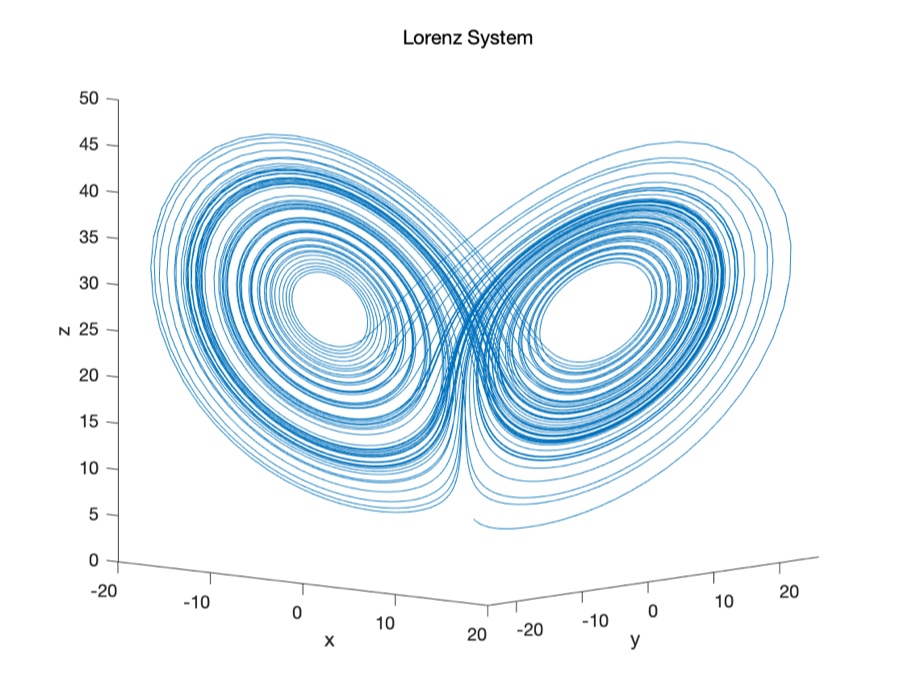
\includegraphics[width=1.6in]{figure/lorenz_phase}
				\caption{Lorenz System相图}
			\end{minipage}
		\end{figure}
		\end{frame}
	
		\begin{frame}{Lorenz System的本征函数}
			\begin{figure}
				\centering
				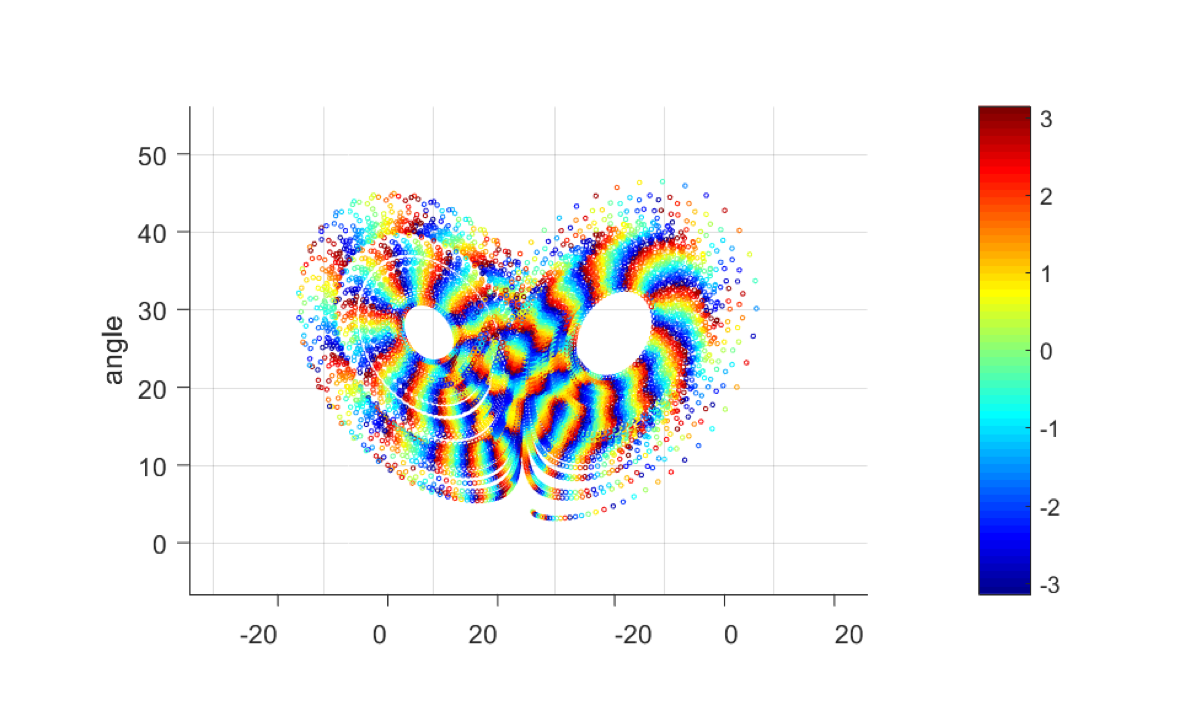
\includegraphics[width=3.5in]{figure/lorenz_eigen}
				\caption{Lorenz System的本征函数}
			\end{figure}
		\end{frame}
		
		\begin{frame}{Lorenz System的本征函数}
			\begin{figure}
				\centering
				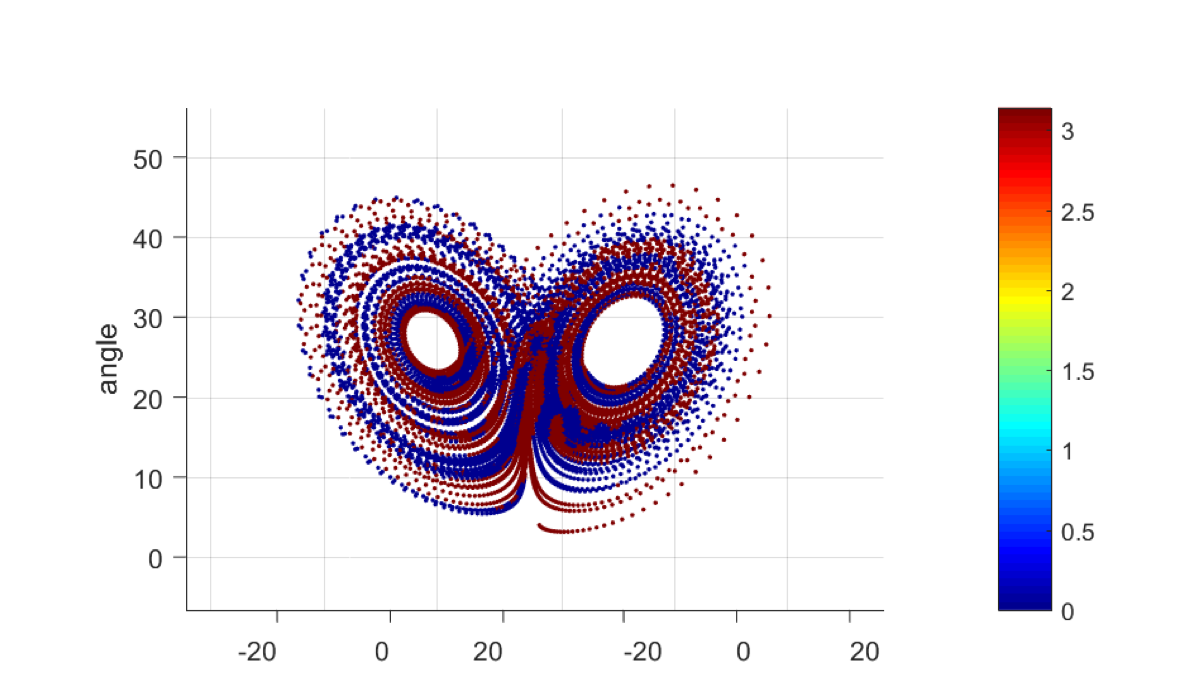
\includegraphics[width=3.5in]{figure/lorenz_eigen_bin}
				\caption{Lorenz System的本征函数}
			\end{figure}
		\end{frame}


\section{总结与展望}
\begin{frame}{总结与展望}
	\begin{enumerate}
		\small
		\item Koopman算符描述了相空间中可观测函数的演化,可用于挖掘重要的动力学模式。
		\item 本征函数值相等的点属于一个不变集。在动力学系统中,不变集与不动点和周期轨道密切相关。
		\item 本征函数的极值与混沌系统中的符号动力学边界点非常吻合,可以通过构造一组基函数来计算Koopman算符谱,且自然基函数相比高斯基函数更有效。
		\item 符号动力学的划分可以预测系统的长期行为。Koopman算符本征函数的极值点为寻找符号动力学的边界点提供了一个有效的数学工具,通过计算谱特征而避免对相空间中复杂的几何特征和拓扑结构进行描述,并可以拓展到复杂的非线性系统。
		\item 基函数和基函数的数量影响本征函数的计算精度,随着基函数数量的增加,本征函数出现了新的层次的边界点,可以通过控制基函数数量对寻找边界点进行粗粒度或细粒度的处理。
		\item 具有普适性与鲁棒性。
	\end{enumerate}
\end{frame}

\begin{frame}{致谢}
\centering
\huge 感谢各位老师莅临指导\\[30pt]
\normalsize 北京邮电大学理学院\\
张聪
\end{frame}
\end{document}
